\chapter{Libraries}\label{HOLlibraries}

% LaTeX macros in HOL manuals
%
% \holtxt{..}     for typewriter text that is HOL types or terms.  To
%                 produce backslashes, for /\, \/ and \x. x + 1, use \bs
% \ml{..}         for typewriter text that is ML input, including the
%                 names of HOL API functions, such as mk_const
% \theoryimp{..}  for names of HOL theories.

% text inside \begin{verbatim} should be indented three spaces, unless
% the verbatim is in turn inside a \begin{session}, in which case it
% should be flush with the left margin.


\newcommand{\simpset}{simpset}
\newcommand{\Simpset}{Simpset}

{
 \newcommand{\term}      {\mbox{\it term}}
 \newcommand{\vstr}      {\mbox{\it vstr}}

A \emph{library} is an abstraction intended to provide a higher level
of organization for \HOL{} applications. In general, a library can
contain a collection of theories, proof procedures, and supporting
material, such as documentation. Some libraries simply provide proof
procedures, such as \ml{simpLib}, while others provide theories and
proof procedures, such as \ml{intLib}. Libraries can include other
libraries.

In the \HOL{} system, libraries are represented by \ML{} structures
named following the convention that library \emph{x} will be found in
the \ML{} structure \ml{xLib}. Loading this structure should load all
the relevant sub-components of the library and set whatever system
parameters are suitable for use of the library.

When the \HOL{} system is invoked in its normal configuration, several
useful libraries are automatically loaded. The most basic \HOL{}
library is \ml{boolLib}, which supports the definitions of
the \HOL{} logic, found in the theory \theoryimp{bool}, and provides a
useful suite of definition and reasoning tools.

Another pervasively used library is found in the structure \ml{Parse}
(the reader can see that we are not strictly faithful to our
convention about library naming). The parser library provides support
for parsing and `pretty-printing' of \HOL{} types, terms, and
theorems.

The \ml{boss} library provides a basic collection of standard
theories and high-level proof procedures, and serves as a standard
platform on which to work. It is preloaded and opened when the \HOL{}
system starts up. It includes \ml{boolLib} and
\ml{Parse}. Theories provided include \theoryimp{pair},
\theoryimp{sum}, \theoryimp{option}; the arithmetic theories
\theoryimp{num}, \theoryimp{prim\_rec}, \theoryimp{arithmetic},
and \theoryimp{numeral}; and \theoryimp{list}. Other libraries
included in \ml{bossLib} are \ml{goalstackLib}, which provides
a proof manager for tactic proofs; \ml{simpLib}, which provides
a variety of simplifiers; \ml{numLib}, which provides a decision
procedure for arithmetic; \ml{Datatype}, which provides
high-level support for defining algebraic datatypes; and \ml{tflLib},
which provides support for defining recursive functions.


\section{Parsing and Prettyprinting}
\label{sec:parsing-printing}

Every type and term in \HOL{} is ultimately built by application of
the primitive (abstract) constructors for types and terms. However, in
order to accomodate a wide variety of mathematical expression, \HOL{}
provides flexible infrastracture for parsing and prettyprinting types
and terms through the \ml{Parse} structure.

The term parser supports type inference, overloading, binders, and
various fixity declaration (infix, prefix, postfix, and
combinations). There are also flags for controlling the behaviour
of the parser. Further, the structure of the parser is exposed so that
new parsers can be quickly constructed to support user applications.

The parser is parameterized by grammars for types and terms. The
behaviour of the parser and prettyprinter is therefore usually altered
by grammar manipulations. These can be of two kinds: \emph{temporary}
or \emph{permanent}.  Temporary changes do not persist after the
current session, while permanent changes will be in force in all
descendant theories.  Functions making temporary alterations are
signified by a leading \ml{temp\_} in their names.

\subsection{The type parser}

The language of types is a simple one.  An abstract grammar for the
language is presented in Figure~\ref{fig:abstract-type-grammar}.  The
actual grammar (with concrete values for the infix symbols and type
operators) can be inspected using the function \ml{type\_grammar}.
\begin{figure}[tbhp]
\newcommand{\nt}[1]{\mathit{#1}}
\newcommand{\tok}[1]{\texttt{\bfseries #1}}
\renewcommand{\bar}{\;\;|\;\;}
\[
\begin{array}{lcl}
\tau &::=& \tau \odot \tau \bar \nt{vtype} \bar \nt{tyop} \bar
           \tok{(} \;\nt{tylist}\;\tok{)} \;\nt{tyop}\bar \tau \;\nt{tyop}
           \bar \tok{(}\;\tau\;\tok{)}\\
\odot &::=& \tok{->} \bar \tok{\#} \bar \tok{+} \bar \cdots\\
\nt{vtype} &::=& \tok{'a} \bar \tok{'b} \bar \tok{'c} \bar \cdots\\
\nt{tylist} &::=& \tau \bar \tau \;\tok{,}\;\nt{tylist}\\
\nt{tyop} &::=& \tok{bool} \bar \tok{list} \bar \tok{num} \bar
           \tok{fun} \bar \cdots
\end{array}
\]
\caption{An abstract grammar for \HOL{} types ($\tau$).  Infixes ($\odot$)
  always bind more weakly than type operators ($\nt{tyop}$), so that
  $\tau_1 \,\odot\, \tau_2 \,\nt{tyop}$ is always parsed as $\tau_1\, \odot\,
  (\tau_2 \,\nt{tyop})$.  Different infixes can have different
  priorities, and infixes at different priority levels can associate
  differently (to the left, to the right, or not at all).  Users can
  extend the categories $\odot$ and $\nt{tyop}$ by making new type
  definitions, and by directly manipulating the grammar.}
\label{fig:abstract-type-grammar}
\end{figure}

\paragraph{Type infixes}
Infixes may be introduced with the function \ml{add\_infix\_type}.
This sets up a mapping from an infix symbol (such as \texttt{->}) to
the name of an existing type operator (such as \texttt{fun}).  The
binary symbol needs to be given a precedence level and an
associativity. See \REFERENCE{} for more details.

\paragraph{Type abbreviations}
\index{type abbreviations}

Users can abbreviate common type patterns with \emph{abbreviations}.
This is done with the \ML{} function \ml{type\_abbrev}:
\begin{hol}
\begin{verbatim}
   type_abbrev : string * hol_type -> unit
\end{verbatim}
\end{hol}
An abbreviation is a new type operator, of any number of arguments,
that expands into an existing type.  For example, one might develop a
light-weight theory of numbers extended with an infinity, where the
represeting type was \holtxt{num option} (\holtxt{NONE} would
represent the infinity value).  One might set up an abbreviation
\holtxt{infnum} that expanded to this underlying type.

Polymorphic patterns are supported as well.  For example, as described
in Section~\ref{sec:theory-of-sets}, the abbreviation \holtxt{set}, of
one argument, is such that \holtxt{:'a set} expands into the type
\holtxt{:'a -> bool}, for any type \holtxt{:'a}.

When types come to be printed, the expansion of abbreviations done by
the parser is reversed.  For more information see the documentation of
\ml{type\_abbrev} in the \REFERENCE.

\subsection{The term parser}

The term parser provides a grammar-based infrastructure for supporting
concrete syntax for formalizations. Usually, the \HOL{} grammar gets
extended when a new definition or constant specification is made. (The
introduction of new constants is discussed in
Sections~\ref{sec:constant-definitions} and \ref{conspec}.) However,
any identifier can have a parsing status attached at any time.
In the following, we explore some of the capabilities of the
\HOL{} term parser.


\subsubsection{Type constraints}

A term can be constrained to be of a certain type.  For example,
\holtxt{X:bool} constrains the variable \holtxt{X} to have type
\holtxt{bool}. An attempt to constrain a
term inappropriately will raise an exception: for example,
\begin{hol}
\begin{verbatim}
   if T then (X:ind) else (Y:bool)
\end{verbatim}
\end{hol}
will fail because both branches of a conditional must be of the same
type.  Type constraints can be seen as a suffix that binds more
tightly than everything except function application.  Thus $\term\
\ldots\ \term \ : \type$ is equal to $(\term\ \ldots\ \term)\ :
\type$, but $x < y:\holtxt{num}$ is a legitimate constraint on just
the variable $y$.

The inclusion of \holtxt{:} in the symbolic identifiers means that some
constraints may need to be separated by white space. For example,
\begin{hol}
\begin{verbatim}
   $=:bool->bool->bool
\end{verbatim}
\end{hol}
will be broken up by the \HOL{} lexer as
\begin{hol}
\begin{verbatim}
   $=: bool -> bool -> bool
\end{verbatim}
\end{hol}
and parsed as an application of the symbolic identifier \holtxt{\$=:} to
the argument list of terms [\holtxt{bool}, \holtxt{->}, \holtxt{bool},
\holtxt{->}, \holtxt{bool}]. A well-placed space will avoid this problem:
\begin{hol}
\begin{verbatim}
   $= :bool->bool->bool
\end{verbatim}
\end{hol}
is parsed as the symbolic identifier ``='' constrained by a type.
Instead of the \holtxt{\$}, one can also use parentheses to remove
special parsing behaviour from lexemes:
\begin{hol}
\begin{verbatim}
   (=):bool->bool->bool
\end{verbatim}
\end{hol}

\subsubsection{Type inference}

Consider the term \holtxt{x = T}: it (and all of its subterms)
has a type in the \HOL{} logic. Now, \holtxt{T} has type \holtxt{bool}. This
means that the constant \holtxt{=} has type \holtxt{xty -> bool -> bool},
for some type \holtxt{xty}. Since the type scheme for \holtxt{=} is
\holtxt{'a -> 'a -> bool}, we know that \holtxt{xty} must in fact be
\holtxt{bool} in order for the type instance to be well-formed. Knowing
this, we can deduce that the type of \holtxt{x} must be \holtxt{bool}.

Ignoring the jargon (``scheme'' and ``instance'') in the previous
paragraph, we have conducted a type assignment to the term structure,
ending up with a well-typed term. It would be very tedious for users
to conduct such argumentation by hand for each term entered to \HOL{}.
Thus, \HOL{} uses an adaptation of Milner's type inference algorithm
for \ML{} when constructing terms via parsing. At the end of type
inference, unconstrained type variables get assigned names by the system.
Usually, this assignment does the right thing. However, at times, the
most general type is not what is desired and the user must add type
constraints to the relevant subterms. For tricky situations, the
global variable \ml{show\_types} can be assigned. When this flag is
set, the prettyprinters for terms and theorems will show how types
have been assigned to subterms. If you do not want the system to
assign type variables for you, the global variable
\ml{guessing\_tyvars} can be set to \ml{false}, in which case the
existence of unassigned type variables at the end of type inference
will raise an exception.


\subsubsection{Overloading}

A limited amount of overloading resolution is performed by the term
parser. For example, the `tilde' symbol (\holtxt{\~{}})
denotes boolean negation in the initial theory of \HOL, and it also denotes
the additive inverse in the \ml{integer} and
\ml{real} theories. If we load the \ml{integer}
theory and enter an ambiguous term featuring \holtxt{\~{}}, the
system will inform us that overloading resolution is being performed.

\setcounter{sessioncount}{1}
\begin{session}
\begin{hol}
\begin{verbatim}
- load "integerTheory";
> val it = () : unit

- Term `~~x`;
<<HOL message: more than one resolution of overloading was possible.>>
> val it = `~~x` : term

- type_of it;
> val it = `:bool` : hol_type
\end{verbatim}
\end{hol}
\end{session}

A priority mechanism is used to resolve multiple possible choices. In
the example, \holtxt{\~{}} could be consistently chosen to have type
\holtxt{:bool -> bool} or \holtxt{:int -> int}, and the
mechanism has chosen the former. For finer control, explicit type
constraints may be used. In the following session, the
\holtxt{\~{}\~{}x} in the first quotation has type \holtxt{:bool},
while in the second, a type constraint ensures that \holtxt{\~{}\~{}x} has
type \holtxt{:int}.

\begin{session}
\begin{hol}
\begin{verbatim}
- show_types := true;
> val it = () : unit

- Term `~(x = ~~x)`;
<<HOL message: more than one resolution of overloading was possible.>>
> val it = `~((x :bool) = ~~x)` : term

- Term `~(x:int = ~~x)`;
> val it = `~((x :int) = ~~x)` : term
\end{verbatim}
\end{hol}
\end{session}

Note that the symbol \holtxt{\~{}} stands for two different constants in
the second quotation; its first occurrence is boolean negation, while
the other two occurrences are the additive inverse operation for integers.
For more information on how to set up and use overloading, consult
\REFERENCE.

\subsubsection{Fixities}

In order to provide some notational flexibility, constants come in
various flavours or {\it fixities}: besides being an ordinary constant
(with a fixity of {\sf Prefix}), constants can also be {\it binders},
{\it true prefixes}\footnote{The use of the term ``true prefix'' is
forced upon us by the history of the system, which reserved the
classification ``prefix'' for terms without any special syntactic
features.}, {\it suffixes}, {\it infixes}, or {\it closefixes}.  More
generally, terms can also be represented using reasonably arbitrary
{\it mixfix} specifications.  The degree to which terms bind their
associated arguments is known as precedence.  The higher this number,
the tighter the binding.  For example, when introduced, \verb-+- has a
precedence of 500, while the tighter binding multiplication (\verb+*+)
has a precedence of 600.

\paragraph{Binders}

A binder is a construct that binds a variable; for example, the
universal quantifier. In \HOL, this is represented using a trick that
goes back to Alonzo Church: a binder is a constant that takes a lambda
abstraction as its argument. The lambda binding is used to implement
the binding of the construct. This is an elegant and uniform solution.
Thus the concrete syntax \verb+!v. M+ is represented by the
application of the constant \verb+!+ to the abstraction \verb+(\v. M)+.

The most common binders are \verb+!+, \verb+?+, \verb+?!+, and
\verb+@+. Sometimes one wants to iterate applications of the same
binder, \eg,
\begin{alltt}
   !x. !y. ?p. ?q. ?r. \term.
\end{alltt}
This can instead be rendered
\begin{alltt}
   !x y. ?p q r. \term.
\end{alltt}

\paragraph{Infixes}

Infix constants can associate in one of three different ways: right,
left or not at all.  (If \holtxt{+} were non-associative, then
\holtxt{3 + 4 + 5} would fail to parse; one would have to write
\holtxt{(3 + 4) + 5} or \holtxt{3 + (4 + 5)} depending on the desired
meaning.)  The precedence ordering for the initial set of infixes is
\holtxt{/\bs}, \holtxt{\bs/}, \holtxt{==>}, \holtxt{=},
\begin{Large}\holtxt{,}\end{Large} (comma\footnote{When
  \theoryimp{pairTheory} has been loaded.}). Moreover, all of these
constants are right associative. Thus
\begin{hol}
\begin{verbatim}
   X /\ Y ==> C \/ D, P = E, Q
\end{verbatim}
\end{hol}
%
is equal to
%
\begin{hol}
\begin{verbatim}
   ((X /\ Y) ==> (C \/ D)), ((P = E), Q).
\end{verbatim}
\end{hol}
%
\noindent An expression
\[
\term \; \holtxt{<infix>}\; \term
\]
is internally represented as
\[
((\holtxt{<infix>}\; \term)\; \term)
\]

\paragraph{True prefixes}

Where infixes appear between their arguments, true prefixes appear
before theirs.  This might initially appear to be the same thing as
happens with normal function application (is $f$ in $f(x)$ not acting
as a prefix?), but in fact, it is useful to allow for prefixes to have
binding power less than that associated with function application.  An
example of this is \verb+~+, logical negation.  This is a prefix with
lower precedence than function application.  Normally
\[
   f\;x\; y\qquad \mbox{is parsed as}\qquad (f\; x)\; y
\] but \[
  \holtxt{\~{}}\; x\; y\qquad\mbox{is parsed as}\qquad
  \holtxt{\~{}}\; (x\; y)
\] because the precedence of \verb+~+ is lower than that of function
application.  The unary negation symbol would also typically be
defined as a true prefix, if only to allow one to write \[ {\it
  negop}\,{\it negop}\,3
\] (whatever {\it negop} happened to be) without needing extra parentheses.

\paragraph{Suffixes}

Suffixes appear after their arguments.  There are no suffixes
introduced into the standard theories available in \HOL{}, but users
are always able to introduce their own if they choose.  Suffixes are
associated with a precedence just as infixes and true prefixes are.
If \holtxt{p} is a true prefix, \holtxt{i} an infix, and \holtxt{s} a
suffix, then there are six possible orderings for the three different
operators based on their precedences, giving five parses for
$\holtxt{p}\; t_1\; \holtxt{i}\; t_2\; \holtxt{s}$ depending on the
relative precedences:
\[
\begin{array}{cl}
\mbox{\begin{tabular}{c}Precedences\\(lowest to highest)\end{tabular}} &
\multicolumn{1}{c}{\mbox{Parses}}\\
\hline
p,\;i,\;s & \holtxt{p}\;(t_1\;\holtxt{i}\;(t_2\;\holtxt{s}))\\
p,\;s,\;i & \holtxt{p}\;((t_1\;\holtxt{i}\;t_2)\;\holtxt{s})\\
i,\;p,\;s & (\holtxt{p}\;t_1)\;\holtxt{i}\;(t_2\;\holtxt{s})\\
i,\;s,\;p & (\holtxt{p}\;t_1)\;\holtxt{i}\;(t_2\;\holtxt{s})\\
s,\;p,\;i & (\holtxt{p}\;(t_1\;\holtxt{i}\;t_2))\;\holtxt{s}\\
s,\;i,\;p & ((\holtxt{p}\;t_1)\;\holtxt{i}\;t_2)\;\holtxt{s}\\
\end{array}
\]

\paragraph{Closefixes}

Closefix terms are operators that completely enclose their arguments.
An example one might use in the development of a theory of
denotational semantics is semantic brackets.  Thus, the \HOL{} parsing
facilities can be configured to allow one to write \holtxt{denotation x}
as \holtxt{[| x |]}.  Closefixes are not associated with precedences
because they can not compete for arguments with other operators.


\subsubsection{Parser tricks and magic}

Here we describe how to achieve some useful effects with the
parser in \HOL{}.

\begin{description}

\item[Aliasing] If one wants a special syntax to be an ``alias'' for a
  normal \HOL{} form, this is easy to achieve; both examples so far
  have effectively done this.  However, if one just wants to have a
  normal one-for-one substitution of one string for another, one can't
  use the grammar/syntax phase of parsing to do this.  Instead, one
  can use the overloading mechanism.  For example, let us alias
  \texttt{MEM} for \texttt{IS\_EL}.  We need to use the function
  \texttt{overload\_on} to overload the original constant for the new
  name:
\begin{hol}
\begin{verbatim}
   val _ = overload_on ("MEM", Term`IS_EL`);
\end{verbatim}
\end{hol}

\item[Making addition right associative] If one has a number of old
  scripts that assume addition is right associative because this is
  how \HOL{} used to be, it might be too much pain to convert.  The trick
  is to remove all of the rules at the given level of the grammar, and
  put them back as right associative infixes.  The easiest way to tell
  what rules are in the grammar is by inspection (use
  \ml{term\_grammar()}).  With just \ml{arithmeticTheory}
  loaded, the only infixes at level 500 are \holtxt{+} and
  \holtxt{-}.  So, we remove the rules for them:
\begin{hol}
\begin{verbatim}
   val _ = app temp_remove_rules_for_term ["+", "-"];
\end{verbatim}
\end{hol}
  \noindent And then we put them back with the appropriate
  associativity:
\begin{hol}
\begin{verbatim}
   val _ = app (fn s => temp_add_infix(s, 500, RIGHT)) ["+", "-"];
\end{verbatim}
\end{hol}
\noindent Note that we use the \ml{temp\_} versions of these two
functions so that other theories depending on this one won't be
affected.  Further note that we can't have two infixes at the same
level of precedence with different associativities, so we have to
remove both operators, not just addition.

\item[Mix-fix syntax for {\it if-then-else}:]
\index{conditionals, in HOL logic@conditionals, in \HOL{} logic!printing of}
%
The first step in bringing this about is to look at the general shape
of expressions of this form.  In this case, it will be:
%
\[
  \holtxt{if}\;\; \dots \;\;\holtxt{then}\;\;\dots\;\;
  \holtxt{else}\;\;\dots
  \]
%
 Because there needs to be a ``dangling'' term to the right, the
  appropriate fixity is \ml{TruePrefix}.  Knowing that the underlying
  term constant is called \holtxt{COND}, the simplest way to achieve
  the desired syntax is:
\begin{hol}
\begin{verbatim}
  val _ = add_rule
        {term_name = "COND", fixity = TruePrefix 70,
         pp_elements = [TOK "if", BreakSpace(1,0), TM, BreakSpace(1,0),
                        TOK "then", BreakSpace(1,0), TM, BreakSpace(1,0),
                        TOK "else", BreakSpace(1,0)],
         paren_style = Always,
         block_style = (AroundEachPhrase, (PP.CONSISTENT, 0))};
\end{verbatim}
\end{hol}
\noindent The actual rule is slightly more complicated, and
may be found in the sources for the theory \theoryimp{bool}.

\item[Mix-fix syntax for term substitution:]

Here the desire is to be able to write something like:
\[
  \mbox{\texttt{[}}\,t_1\,\mbox{\texttt{/}}\,t_2\,\mbox{\texttt{]}}\,t_3
\]
denoting the substitution of $t_1$ for $t_2$ in $t_3$, perhaps
translating to \holtxt{SUB $t_1$ $t_2$ $t_3$}.  This looks
like it should be another \ml{TruePrefix}, but the choice of the
square brackets (\holtxt{[} and \holtxt{]}) as delimiters would
conflict with the concrete syntax for list literals if this was done.
Given that list literals are effectively of the \ml{CloseFix}
class, the new syntax must be of the same class.  This is easy enough
to do: we set up syntax
\[
\holtxt{[}\,t_1\,\holtxt{/}\,t_2\,\holtxt{]}
\]
to map to \holtxt{SUB $t_1$ $t_2$}, a value of a functional
type, that when applied to a third argument will look
right.\footnote{Note that doing the same thing for the
  \textit{if-then-else} example in the previous example would be
  inappropriate, as it would allow one to write
\[ \holtxt{if}\;P\;\holtxt{then}\;Q\;\holtxt{else} \]
without the trailing argument.}
The rule for this is thus:
\begin{hol}
\begin{verbatim}
  val _ = add_rule
           {term_name = "SUB", fixity = Closefix,
            pp_elements = [TOK "[", TM, TOK "/", TM, TOK "]"],
            paren_style = OnlyIfNecessary,
            block_style = (AroundEachPhrase, (PP.INCONSISTENT, 2))};
\end{verbatim}
\end{hol}

\end{description}

\subsubsection{Hiding constants}
\label{hidden}

\index{parsing, of HOL logic@parsing, of \HOL{} logic!hiding constant status in|(}
\index{HOL system@\HOL{} system!hiding constants in|(}
\index{constants, in HOL logic@constants, in \HOL{} logic!hiding status of}
%
The following function can be used to hide the constant status of a
name from the quotation parser.

\begin{boxed}
\index{hide@\ml{hide}|pin}
\begin{verbatim}
  val hide   : string -> ({Name : string, Thy : string} list *
                          {Name : string, Thy : string} list)
\end{verbatim}
\end{boxed}

\noindent Evaluating \ml{hide "$x$"}
makes the quotation parser treat $x$ as a variable (lexical
rules permitting), even if $x$ is the name of a constant in the current theory
(constants and variables can have the same name).
This is useful if one wants to use variables
%
\index{variables, in HOL logic@variables, in \HOL{} logic!with constant names}
%
with the same names as previously declared (or built-in) constants
(\eg\ \ml{o}, \ml{I}, \ml{S} \etc).  The name $x$ is still a constant
for the constructors, theories, etc; \ml{hide} affects only parsing.
See the \REFERENCE{} entry for \ml{hide} for more details, including
an explanation of the return type.

The function

\begin{boxed}
\index{reveal@\ml{reveal}|pin}
\begin{verbatim}
   reveal : string -> unit
\end{verbatim}
\end{boxed}

\noindent undoes hiding.

The function

\begin{boxed}
\index{hidden@\ml{hidden}|pin}
\begin{verbatim}
   hidden : string -> bool
\end{verbatim}
\end{boxed}

\noindent tests whether a string is the name of a hidden constant.
\index{HOL system@\HOL{} system!adjustment of user interface of}
\index{HOL system@\HOL{} system!hiding constants in|)}
\index{parsing, of HOL logic@parsing, of \HOL{} logic!hiding constant status in|)}

\subsubsection{Adjusting the pretty-print depth}
\index{printing, in HOL logic@printing, in \HOL{} logic!structural depth adjustment in}

The following \ML{} reference can be used to adjust the maximum depth
of printing

\begin{boxed}
\index{max_print_depth@\ml{max\_print\_depth}|pin}
\begin{verbatim}
   max_print_depth : int ref
\end{verbatim}
\end{boxed}

\index{default print depth, for HOL logic@default print depth, for \HOL{} logic|(}

\noindent The default print depth is $-1$, which is interpreted as
meaning no maximum.  Subterms nested more deeply than the maximum
print depth are printed as \holtxt{...}. For example:

\setcounter{sessioncount}{0}
\begin{session}
\begin{hol}
\begin{verbatim}
- ADD_CLAUSES;
> val it =
    |- (0 + m = m) /\ (m + 0 = m) /\ (SUC m + n = SUC (m + n)) /\
       (m + SUC n = SUC (m + n)) : thm

- max_print_depth := 3;
> val it = () : unit
- ADD_CLAUSES;
> val it = |- (... + ... = m) /\ (... = ...) /\ ... /\ ... : thm
\end{verbatim}
\end{hol}
\end{session}
\index{default print depth, for HOL logic@default print depth, for \HOL{} logic|)}

\subsection{Quotations and Antiquotation}
\label{sec:quotation-antiquotation}

\index{quotation, in HOL logic@quotation, in \HOL{} logic!parser for}
\index{parsing, of HOL logic@parsing, of \HOL{} logic!of quotation syntax|(}
Logic-related syntax in the HOL system is typically passed to the
parser in special forms known as \emph{quotations}.  A basic quotation
is delimited by single back-ticks (i.e., \ml{`}, ASCII character~96).  When
quotation values are printed out by the ML interactive loop, they look
rather ugly because of the special filtering that is done to these
values before the ML interpreter even sees them:
\setcounter{sessioncount}{0}
\begin{session}
\begin{hol}
\begin{verbatim}
- val q = `f x = 3`;
> val 'a q = [QUOTE " (*#loc 1 11*)f x = 3"] : 'a frag list
\end{verbatim}
\end{hol}
\end{session}
Quotations (Moscow ML prints the type as \ml{'a frag list}) are the
raw input form expected by the various HOL parsers.  They are also
polymorphic (to be explained below).  Thus the function
\ml{Parse.Term} function takes a (term) quotation and returns a term,
and is thus of type \[ \ml{term quotation -> term}
\]

The term and type parsers can also be called implicitly by using
double back-ticks as delimiters.  For the type parser, the first
non-space character after the leading delimiter must also be a colon.
Thus:
\begin{session}
\begin{hol}
\begin{verbatim}
- val t = ``p /\ q``;
> val t = ``p /\ q`` : term

- val ty = ``:'a -> bool``;
> val ty = ``:'a -> bool`` : hol_type
\end{verbatim}
\end{hol}
\end{session}

The expression bound to ML variable \ml{t} above is actually expanded
to an application of the function \ml{Parse.Term} to the quotation
argument \ml{`p /\bs{} q`}.  Similarly, the second expression expands
into an application of \ml{Parse.Type} to the quotation \ml{`:'a -> bool`}.

The significant advantage of quotations over normal \ML{} strings is
that they can include new-line and backslash characters without
requiring special quoting.  Newlines occur whenever terms get beyond
the trivial in size, while backslashes occur in not just the
representation of $\lambda$, but also the syntax for conjunction and
disjunction.

If a quotation is to include a back-quote character, then this should
be done by using the quotation syntax's own escape character, the
caret (\ml{\^}, ASCII character~94).  To get a bare caret, things are
slightly more complicated.  If a sequence of carets is followed by
white-space (including a newline), then that sequence of carets is
passed to the HOL parser unchanged.  Otherwise, one caret can be
obtained by writing two in a row. (This last rule is analogous to the
way in \ML{} string syntax treats the back-slash.) Thus:
\begin{session}
\begin{hol}
\begin{verbatim}
- ``f ^` x ``;
<<HOL message: inventing new type variable names: 'a, 'b, 'c>>
> val it = ``f ` x`` : term

- ``f ^ x``;
<<HOL message: inventing new type variable names: 'a, 'b, 'c>>
> val it = ``f ^ x`` : term
\end{verbatim}
\end{hol}
\end{session}

The rule for carets not followed by white-space is illustrated here,
including an example of what happens when the quoting rule is not
followed:
\begin{session}
\begin{hol}
\begin{verbatim}
- ``f ^^+ x``;
<<HOL message: inventing new type variable names: 'a, 'b, 'c>>
> val it = ``f ^+ x`` : term

- ``f ^+ x``;
! Toplevel input:
! (Parse.Term [QUOTE " (*#loc 2 3*)f ", ANTIQUOTE (+),
!              QUOTE " (*#loc 2 7*) x"]);
!                                                  ^
! Ill-formed infix expression
\end{verbatim}
\end{hol}
\end{session}

The main use of the caret is to introduce \emph{antiquotations} (as
suggested in the last example above).  Within a quotation, expressions
of the form {\small\verb+^(+}$t${\small\verb+)+}
%
\index{ antiquotation, in HOL logic@{\small\verb+^+} (antiquotation, in \HOL{} logic)}
%
(where $t$ is an \ML\ expression of type
%
\index{type checking, in HOL logic@type checking, in \HOL{} logic!antiquotation in}
%
\ml{term} or \ml{type}) are called antiquotations.
%
\index{terms, in HOL logic@terms, in \HOL{} logic!antiquotation}
\index{antiquotation, in HOL logic terms@antiquotation, in \HOL{} logic terms}
%
An antiquotation \holtxt{\^{}($t$)} evaluates to the
\ML{} value of $t$. For example,{\small\verb+``x \/ ^(mk_conj(``y:bool``, ``z:bool``))``+}
evaluates to the same term as {\small\verb+``x \/ (y /\ z)``+}. The
most common use of antiquotation is when the term $t$ is bound to an \ML\
variable $x$. In this case {\small\verb+^(+}$x${\small\verb+)+} can be
abbreviated by {\small\verb+^+}$x$.

The following session illustrates antiquotation.

\setcounter{sessioncount}{0}
\begin{session}
\begin{hol}
\begin{verbatim}
- val y = ``x+1``;
> val y = ``x + 1`` : term

val z = ``y = ^y``;
> val z = ``y = x + 1`` : term

- ``!x:num.?y:num.^z``;
> val it = ``!x. ?y. y = x + 1`` : term
\end{verbatim}
\end{hol}
\end{session}

\noindent Types may be antiquoted as well:

\begin{session}
\begin{hol}
\begin{verbatim}
- val pred = ``:'a -> bool``;
> val pred = ``:'a -> bool`` : hol_type

- ``:^pred -> bool``;
> val it = ``:('a -> bool) -> bool`` : hol_type
\end{verbatim}
\end{hol}
\end{session}

\noindent Quotations are polymorphic, and the type variable of a
quotation corresponds to the type of entity that can be antiquoted
into that quotation.  Because the term parser expects only antiquoted
terms, antiquoting a type into a term quotation requires the use of
\holtxt{ty\_antiq}. For example,%
%
\index{ty_antiq@\ml{ty\_antiq}}

\begin{session}
\begin{hol}
\begin{verbatim}
- ``!P:^pred. P x ==> Q x``;

! Toplevel input:
! Term `!P:^pred. P x ==> Q x`;
!           ^^^^
! Type clash: expression of type
!   hol_type
! cannot have type
!   term

- ``!P:^(ty_antiq pred). P x ==> Q x``;
> val it = `!P. P x ==> Q x` : term
\end{verbatim}
\end{hol}
\end{session}
%
\index{parsing, of HOL logic@parsing, of \HOL{} logic!of quotation syntax|)}



\subsection{Backwards compatibility of syntax}

This section of the manual documents the (extensive) changes made to
the parsing of \HOL{} terms and types in the Taupo release (one of the
HOL3 releases) and beyond from the point of view of a user who doesn't
want to know how to use the new facilities, but wants to make sure
that their old code continues to work cleanly.

The changes which may cause old terms to fail to parse are:
\begin{itemize}
\newcommand\condexp{\holtxt{$p$ => $q$ | $r$}}
\item The precedence of type annotations has completely changed.  It
  is now a very tight suffix (though with a precedence weaker than
  that associated with function application), instead of a weak one.
  This means that \mbox{\tt (x,y:bool \# bool)} should now be written
  as \mbox{\tt (x,y):bool \# bool}. The previous form will now be
  parsed as a type annotation applying to just the \verb+y+.  This
  change brings the syntax of the logic closer to that of SML and
  should make it generally easier to annotate tuples, as one can now
  write \[ (x\,:\,\tau_1,\;y\,:\,\tau_2,\dots z\,:\,\tau_n)
  \] instead of \[
  (x\,:\,\tau_1, \;(y\,:\,\tau_2, \dots (z\,:\,\tau_n)))
  \] where extra parentheses have had to be added just to allow one to
  write a frequently occurring form of constraint.
\item Most arithmetic operators are now left associative instead of
  right associative.  In particular, $+$, $-$, $*$ and {\tt DIV} are
  all left associative.  Similarly, the analogous operators in other
  numeric theories such as {\tt integer} and {\tt real} are also left
  associative.  This brings the \HOL{} parser in line with standard
  mathematical practice.
\item The binding equality in {\tt let} expressions is treated exactly
  the same way as equalities in other contexts.  In previous versions
  of \HOL, equalities in this context have a different, weak binding
  precedence.  This difference can be seen in the following expression
  which parses successfully in the old version:
  \[ {\tt let} \; x \; = \; \condexp \; {\tt
  in} \;Q \] In Taupo releases and later, this expression will not
  parse because the conditional expression binds to the left more
  weakly than the equality binds to the right, and the parser ends up
  believing that the binding between the \verb+let+ and the \verb+in+
  is not an equality after all, as it should be.
\item Old style conditional expressions in the right half of set
  comprehensions have to be parenthesised to avoid confusing the
  parser.  Thus \[
  \{ \; x \; | \; \condexp \; \}
   \qquad\mbox{must be written} \qquad
  \{ \; x \; | \; (\condexp) \; \}
  \] Better yet, {\tt if}-{\tt then}-{\tt else} syntax could be used
  for the conditional expression.
\item Some lexical categories are more strictly policed.  String
  literals (strings inside double quotes) and numerals can't be used
  unless the relevant theories have been loaded.  Nor can these
  literals be used as variables inside binding scopes.
\end{itemize}


\section{A Simple Interactive Proof Manager}\label{sec:goalstack}

The \emph{goal stack} provides a simple interface to tactic-based
interactive proof. When one uses tactics to decompose a proof, many
intermediate states arise; the goalstack takes care of the necessary
bookeeping. The implementation of goalstacks reported here is a
re-design of Larry Paulson's original conception.

The goalstack library is automatically loaded when \HOL{} starts up.

The abstract types \ml{goalstack} and \ml{proofs} are the
focus of backwards proof operations. The type \ml{proofs} can be
regarded as a list of independent goalstacks. Most operations act on
the head of the list of goalstacks; there are also operations so that
the focus can be changed.

\subsection{Starting a goalstack proof}

\begin{hol}
\begin{verbatim}
   g        : term quotation -> proofs
   set_goal : goal -> proofs
\end{verbatim}
\end{hol}

Recall that the type \ml{goal} is an abbreviation for
\ml{term list * term}. To start on a new goal, one gives
\ml{set\_goal} a goal. This creates a new goalstack and makes it the
focus of further operations.

A shorthand for \ml{set\_goal} is the function \ml{g}: it
invokes the parser automatically, and it doesn't allow the the goal to
have any assumptions.

Calling \ml{set\_goal}, or \ml{g}, adds a new proof attempt to the
existing ones, \textit{i.e.}, rather than overwriting the current
proof attempt, the new attempt is stacked on top.

\subsection{Applying a tactic to a goal}

\begin{hol}
\begin{verbatim}
   expandf : tactic -> goalstack
   expand  : tactic -> goalstack
   e       : tactic -> goalstack
\end{verbatim}
\end{hol}

How does one actually do a goalstack proof then? In most cases, the
application of tactics to the current goal is done with the function
\verb+expand+. In the rare case that one wants to apply an
{\it invalid\/} tactic, then \verb+expandf+ is used. (For an
explanation of invalid tactics, see Chapter 24 of Gordon \& Melham.) The
abbreviation \verb+e+ may also be used to expand a tactic.


\subsection{Undo}

\begin{hol}
\begin{verbatim}
   b          : unit -> goalstack
   drop       : unit -> proofs
   dropn      : int  -> proofs
   backup     : unit -> goalstack
   restart    : unit -> goalstack
   set_backup : int  -> unit
\end{verbatim}
\end{hol}

Often (we are tempted to say {\it usually}!) one takes a wrong path
in doing a proof, or makes a mistake when setting a goal. To undo a step
in the goalstack, the function \ml{backup} and its abbreviation
\ml{b} are used. This will restore the goalstack to its previous
state.


To directly back up all the way to the original goal, the function
\ml{restart} may be used. Obviously, it is also important to get
rid of proof attempts that are wrong; for that there is \ml{drop},
which gets rid of the current proof attempt, and \ml{dropn}, which
eliminates the top $n$ proof attempts.


Each proof attempt has its own \emph{undo-list} of previous
states. The undo-list for each attempt is of fixed size (initially
12). If you wish to set this value for the current proof attempt, the
function \ml{set\_backup} can be used. If the size of the backup
list is set to be smaller than it currently is, the undo list will be
immediately truncated. You can not undo a ``proofs-level'' operation, such
as \ml{set\_goal} or \ml{drop}.

\subsection{Viewing the state of the proof manager}

\begin{hol}
\begin{verbatim}
   p            : unit -> goalstack
   status       : unit -> proofs
   top_goal     : unit -> goal
   top_goals    : unit -> goal list
   initial_goal : unit -> goal
   top_thm      : unit -> thm
\end{verbatim}
\end{hol}

To view the state of the proof manager at any time, the functions
\ml{p} and \ml{status} can be used. The former only shows
the top subgoals in the current goalstack, while the second gives a
summary of every proof attempt.

To get the top goal or goals of a proof attempt, use \ml{top\_goal}
and \ml{top\_goals}. To get the original goal of a proof attempt,
use \ml{initial\_goal}.

Once a theorem has been proved, the goalstack that was used to derive it
still exists (including its undo-list): its main job now is to
hold the theorem. This theorem can be retrieved with
\ml{top\_thm}.

\subsection{Switch focus to a different subgoal or proof attempt}

\begin{hol}
\begin{verbatim}
   r             : int -> goalstack
   R             : int -> proofs
   rotate        : int -> goalstack
   rotate_proofs : int -> proofs
\end{verbatim}
\end{hol}

Often we want to switch our attention to a different goal in the current
proof, or a different proof. The functions that do this are
\ml{rotate} and \ml{rotate\_proofs}, respectively. The abbreviations
\ml{r} and \ml{R} are simpler to type in.

\section{High Level Proof---\texttt{bossLib}}
% would use \ml{boss} above but it puts LaTeX into fits
\label{sec:bossLib}
\newcommand\bossLib{\ml{bossLib}}

\index{bossLib@\ml{bossLib}}
The library \bossLib\ marshalls some of the most widely used theorem
proving tools in \HOL{} and provides them with a convenient interface
for interaction. The library currently focuses on three things:
definition of datatypes and functions; high-level interactive proof
operations, and composition of automated reasoners. Loading \bossLib\
commits one to working in a context that already supplies the theories
of booleans, pairs, sums, the option type, arithmetic, and lists.


\subsection{Support for high-level proof steps}
\label{sec:high-level-proof-steps}

The following functions use information in the database to ease the
application of \HOL's underlying functionality:

\begin{verbatim}
   type_rws     : hol_type -> thm list
   Induct       : tactic
   Cases        : tactic
   Cases_on     : term quotation -> tactic
   Induct_on    : term quotation -> tactic
\end{verbatim}

\index{type_rws@\ml{type\_rws}}
\index{TypeBase@\ml{TypeBase}}
%
The function \ml{type\_rws} will search for the given type in the
underlying \ml{TypeBase} database and return useful rewrite rules for
that type. The rewrite rules of the datatype are built from the
injectivity and distinctness theorems, along with the case constant
definition. The simplification tactics \ml{RW\_TAC}, \ml{SRW\_TAC},
and the \simpset{} \ml{(srw\_ss())} automatically include these
theorems.  Other tactics used with other \simpset{}s will need these
theorems to be manually added.

\index{induction theorems, in HOL logic@induction theorems, in \HOL{} logic!for algebraic data types}
%
The \ml{Induct} tactic makes it convenient to invoke induction. When
it is applied to a goal, the leading universal quantifier is examined;
if its type is that of a known datatype, the appropriate structural
induction tactic is extracted and applied.

The \ml{Cases} tactic makes it convenient to invoke case
analysis. The leading universal quantifier in the goal is examined; if
its type is that of a known datatype, the appropriate structural
case analysis theorem is extracted and applied.

The \ml{Cases\_on} tactic takes a quotation, which is
parsed into a term $M$, and then $M$ is searched for in the goal. If $M$
is a variable, then a variable with the same name is searched for. Once
the term to split over is known, its type and the associated facts are
obtained from the underlying database and used to perform the case
split. If some free variables of $M$ are bound in the goal, an attempt
is made to remove (universal) quantifiers so that the case split has
force. Finally, $M$ need not appear in the goal, although it should at
least contain some free variables already appearing in the goal. Note
that the \ml{Cases\_on} tactic is more general than \ml{Cases}, but
it does require an explicit term to be given.

The \ml{Induct\_on} tactic takes a quotation, which is parsed into a
term $M$, and then $M$ is searched for in the goal. If $M$ is a
variable, then a variable with the same name is searched for. Once the
term to induct on is known, its type and the associated facts are
obtained from the underlying database and used to perform the
induction.  If $M$ is not a variable, a new variable $v$ not already
occurring in the goal is created, and used to build a term $v = M$
which the goal is made conditional on before the induction is
performed. First however, all terms containing free variables from $M$
are moved from the assumptions to the conclusion of the goal, and all
free variables of $M$ are universally quantified. \ml{Induct\_on} is
more general than \ml{Induct}, but it does require an explicit term to
be given.

Three supplementary entrypoints have been provided for more exotic
inductions:
\begin{description}
\item [\ml{completeInduct\_on}] performs complete induction on the
  term denoted by the given quotation. Complete induction allows a
  seemingly \footnote{Complete induction and ordinary mathematical
    induction are each derivable from the other.} stronger induction
  hypothesis than ordinary mathematical induction: to wit, when
  inducting on $n$, one is allowed to assume the property holds for
  \emph{all} $m$ smaller than $n$. Formally: $\forall P.\ (\forall x.\
  (\forall y.\ y < x \supset P\, y) \supset P\,x) \supset \forall x.\
  P\,x$. This allows the inductive hypothesis to be used more than
  once, and also allows instantiating the inductive hypothesis to
  other than the predecessor.

\item [\ml{measureInduct\_on}] takes a quotation, and breaks it
  apart to find a term and a measure function with which to induct.
  For example, if one wanted to induct on the length of a list
  \holtxt{L}, the invocation \ml{measureInduct\_on~`LENGTH L`}
  would be be appropriate.

\item [\ml{recInduct}] takes a induction theorem generated by
\ml{Define} or \ml{Hol\_defn} and applies it to the current goal.

\end{description}


\subsection{Automated reasoners}
\label{sec:automated-reasoners}

\ml{bossLib} brings together the most powerful reasoners in \HOL{} and
tries to make it easy to compose them in a simple way. We take our basic
reasoners from \ml{mesonLib}, \ml{simpLib}, and \ml{numLib},
but the point of \ml{bossLib} is to provide a layer of abstraction so
the user has to know only a few entrypoints.\footnote{In the mid 1980's
Graham Birtwistle advocated such an approach, calling it `Ten Tactic
HOL'.} (These underlying libraries, and others providing similarly
powerful tools are described in detail in sections below.)
\begin{hol}
\begin{verbatim}
   PROVE      : thm list -> term -> thm
   PROVE_TAC  : thm list -> tactic

   METIS_TAC  : thm list -> tactic
   METIS_PROVE: thm list -> term -> thm

   DECIDE     : term quotation -> thm
   DECIDE_TAC : tactic
\end{verbatim}
\end{hol}
The inference rule \texttt{PROVE} (and the corresponding tactic
\texttt{PROVE\_TAC}) takes a list of theorems and a term, and attempts
to prove the term using a first order reasoner.  The two \ml{METIS}
functions perform the same functionality but use a different
underlying proof method.  The \texttt{PROVE} entry-points refer to the
\texttt{meson} library, which is further described in
Section~\ref{sec:mesonLib} below. The \ml{METIS} system is described
in Section~\ref{sec:metisLib}.  The inference rule \texttt{DECIDE}
(and the corresponding tactic \texttt{DECIDE\_TAC}) applies a decision
procedure that (at least) handles statements of linear arithmetic.

\begin{hol}
\begin{verbatim}
   RW_TAC   : simpset -> thm list -> tactic
   SRW_TAC  : ssfrag list -> thm list -> tactic
   &&       : simpset * thm list -> simpset  (* infix *)
   std_ss   : simpset
   arith_ss : simpset
   list_ss  : simpset
   srw_ss   : unit -> simpset
\end{verbatim}
\end{hol}
%
\index{RW_TAC@\ml{RW\_TAC}} The rewriting tactic \ml{RW\_TAC} works by
first adding the given theorems into the given \simpset; then it
simplifies the goal as much as possible; then it performs case splits
on any conditional expressions in the goal; then it repeatedly (1)
eliminates all hypotheses of the form $v = M$ or $M = v$ where $v$ is
a variable not occurring in $M$, (2) breaks down any equations between
constructor terms occurring anywhere in the goal. Finally,
\ml{RW\_TAC} lifts \holtxt{let}-expressions within the goal so that
the binding equations appear as
abbreviations\index{abbreviations!tactic-based proof} in the
assumptions.

\index{SRW_TAC@\ml{SRW\_TAC}} The tactic \ml{SRW\_TAC} is similar to
\ml{RW\_TAC}, but works with respect to an underlying \simpset{}
(accessible through the function \ml{srw\_ss}) that is updated as new
context is loaded.  This \simpset{} can be augmented through the
addition of ``\simpset{} fragments'' (\ml{ssfrag} values) and
theorems.  In situations where there are many large types stored in
the system, \ml{RW\_TAC}'s performance can suffer because it
repeatedly adds all of the rewrite theorems for the known types into a
\simpset{} before attacking the goal.  On the other hand,
\ml{SRW\_TAC} loads rewrites into the \simpset{} underneath
\ml{srw\_ss()} just once, making for faster operation in this
situation.

\ml{bossLib} provides a number of simplification sets. The
simpset for pure logic, sums, pairs, and the \ml{option} type is
named \ml{std\_ss}. The simpset for arithmetic is named
\ml{arith\_ss}, and the simpset for lists is named \ml{list\_ss}.
The simpsets provided by \bossLib{} strictly increase in strength:
\ml{std\_ss} is contained in \ml{arith\_ss}, and \ml{arith\_ss} is
contained in \ml{list\_ss}.  The infix combinator \ml{\&\&} is used
to build a new \simpset{} from a given \simpset{} and a list of
theorems. \HOL's simplification technology is described further in
Section~\ref{sec:simpLib} below and in the \REFERENCE.

\begin{hol}
\begin{verbatim}
   by : term quotation * tactic -> tactic (* infix 8 *)
   SPOSE_NOT_THEN : (thm -> tactic) -> tactic
\end{verbatim}
\end{hol}
The function \ml{by} is an infix operator that takes a quotation
and a tactic $tac$. The quotation is parsed into a term $M$. When the
invocation ``\ml{$M$ by $\mathit{tac}$}'' is applied to a goal
$(A,g)$, a new subgoal $(A,M)$ is created and $tac$ is applied to it.
If the goal is proved, the resulting theorem is broken down and added
to the assumptions of the original goal; thus the proof proceeds with
the goal $((M::A), g)$. (Note however, that case-splitting will happen
if the breaking-down of $\ \vdash M$ exposes disjunctions.) Thus
\ml{by} allows a useful style of `assertional' or `Mizar-like'
reasoning to be mixed with ordinary tactic proof.\footnote{Proofs in
  the Mizar system are readable documents, unlike most
  tactic-based proofs.}

The \ml{SPOSE\_NOT\_THEN} entrypoint initiates a proof by
contradiction by assuming the negation of the goal and driving the
negation inwards through quantifiers. It provides the resulting
theorem as an argument to the supplied function, which will use the
theorem to build and apply a tactic.

\section{First Order Proof---\texttt{mesonLib} and \texttt{metisLib}}
\label{sec:first-order-proof}
\index{decision procedures!first-order logic}

First order proof is a powerful theorem-proving technique that can
finish off complicated goals.  Unlike tools such as the simplifier, it
either proves a goal outright, or fails.  It can not transform a goal
into a different (and more helpful) form.

\subsection{Model elimination---\texttt{mesonLib}}
\label{sec:mesonLib}

\index{meson (model elimination) procedure@\ml{meson} (model elimination) procedure}
\index{model elimination method for first-order logic}

The \ml{meson} library is an implementation of the
model-elimination method for finding proofs of goals in first-order
logic.  There are three main entry-points:
\begin{hol}
\begin{verbatim}
   MESON_TAC     : thm list -> tactic
   ASM_MESON_TAC : thm list -> tactic
   GEN_MESON_TAC : int -> int -> int -> thm list -> tactic
\end{verbatim}
\end{hol}

Each of these tactics attempts to prove the goal.  They will either
succeed in doing so, or fail with a ``depth exceeded'' exception.  If
the branching factor in the search-space is high, the \texttt{meson}
tactics may also take a very long time to reach the maximum depth.

All of the \texttt{meson} tactics take a list of theorems.  These
extra facts are used by the decision procedure to help prove the goal.
\texttt{MESON\_TAC} ignores the goal's assumptions; the other two
entry-points include the assumptions as part of the sequent to be
proved.

The extra parameters to \ml{GEN\_MESON\_TAC} provide extra control of
the behaviour of the iterative deepening that is at the heart of the
search for a proof.  In any given iteration, the algorithm searches
for a proof of depth no more than a parameter $d$.  The default
behaviour for \ml{MESON\_TAC} and \ml{ASM\_MESON\_TAC} is to start $d$
at 0, to increment it by one each time a search fails, and to fail if
$d$ exceeds the value stored in the reference value
\ml{mesonLib.max\_depth}.  By way of contrast,
\ml{GEN\_MESON\_TAC~min~max~step} starts $d$ at \ml{min}, increments
it by \ml{step}, and gives up when $d$ exceeds \ml{max}.

The \ml{PROVE\_TAC} function from \ml{bossLib} performs some
normalisation, before passing a goal and its assumptions to
\ml{ASM\_MESON\_TAC}.  Because of this normalisation, in most
circumstances, \ml{PROVE\_TAC} should be preferred to
\ml{ASM\_MESON\_TAC}.

\subsection{Resolution---\texttt{metisLib}}
\label{sec:metisLib}

\index{metis (resolution) procedure@\ml{metis} (resolution) procedure}
\index{resolution method for first-order logic}

The \ml{metis} library is an implementation of the resolution method
for finding proofs of goals in first-order logic. There are two main
entry-points:

\begin{hol}
\begin{verbatim}
   METIS_TAC   : thm list -> tactic
   METIS_PROVE : thm list -> term -> thm
\end{verbatim}
\end{hol}

Both functions take a list of theorems, and these are used as lemmas
in the proof. \texttt{METIS\_TAC} is a tactic, and will either succeed
in proving the goal, or if unsuccessful will either fail or loop
forever. \texttt{METIS\_PROVE} takes a term $t$ and tries to prove a
theorem with conclusion $t$: if successful, the theorem $\vdash t$ is
returned. As for \texttt{METIS\_TAC}, it might fail or loop forever if
the proof search is unsuccessful.

The \texttt{metisLib} family of proof tools implement the ordered
resolution and ordered paramodulation calculus for first order logic,
which usually makes them better suited to goals requiring non-trivial
equality reasoning than the tactics in \texttt{mesonLib}.


\section{Simplification---\texttt{simpLib}}
\label{sec:simpLib}
\index{simplification|(}

The simplifier is \HOL's most sophisticated rewriting engine.  It is
recommended as a general purpose work-horse during interactive
theorem-proving.  As a rewriting tool, the simplifier's general role
is to apply theorems of the general form
\[
\vdash l = r
\]
to terms, replacing instances of $l$ in the term with $r$. Thus, the
basic simplification routine is a \emph{conversion}, taking a term
$t$, and returning a theorem $\vdash t = t'$, or the exception
\ml{UNCHANGED}.

The basic conversion is
\begin{hol}
\begin{verbatim}
   simpLib.SIMP_CONV : simpLib.simpset -> thm list -> term -> thm
\end{verbatim}
\end{hol}
The first argument, a \simpset, is the standard way of providing a
collection of rewrite rules (and other data, to be explained below) to
the simplifier.  There are \simpset{}s accompanying most of \HOL's
major theories.  For example, the \simpset{} \ml{boolSimps.bool\_ss}
embodies all of the usual rewrite theorems one would want over boolean
formulas:
\setcounter{sessioncount}{0}
\begin{session}
\begin{hol}
\begin{verbatim}
- SIMP_CONV bool_ss [] ``p /\ T \/ ~(q /\ r)``;
> val it = |- p /\ T \/ ~(q /\ r) = p \/ ~q \/ ~r : thm
\end{verbatim}
\end{hol}
\end{session}
In addition to rewriting with the obvious theorems, \ml{bool\_ss} is
also capable of performing simplifications that are not expressible as
simple theorems:
\begin{session}
\begin{hol}
\begin{verbatim}
- SIMP_CONV bool_ss [] ``?x. (\y. P (f y)) x /\ (x = z)``;
> val it = |- (?x. (\y. P (f y)) x /\ (x = z)) = P (f z) : thm
\end{verbatim}
\end{hol}
\end{session}
In this example, the simplifier performed a $\beta$-reduction in the
first conjunct under the existential quantifier, and then did an
``unwinding'' or ``one-point'' reduction, recognising that the only
possible value for the quantified variable \holtxt{x} was the value
\holtxt{z}.

The second argument to \ml{SIMP\_CONV} is a list of theorems to be
added to the provided \simpset, and used as additional rewrite rules.
In this way, users can temporarily augment standard \simpset{}s with
their own rewrites.  If a particular set of theorems is often used as
such an argument, then it is possible to build a \simpset{} value to
embody these new rewrites.

For example, the rewrite \ml{arithmeticTheory.LEFT\_ADD\_DISTRIB}, which
states that $p(m + n) = pm + pn$ is not part of any of \HOL's standard
\simpset{}s.  This is because it can cause an unappealing increase in
term size (there are two occurrences of $p$ on the right hand
side of the theorem).  Nonetheless, it is clear that this theorem may
be appropriate on occasion:
\begin{session}
\begin{hol}
\begin{verbatim}
- SIMP_CONV bossLib.arith_ss [LEFT_ADD_DISTRIB] ``p * (n + 1)``;
> val it = |- p * (n + 1) = p + n * p : thm
\end{verbatim}
\end{hol}
\end{session}
Note how the \ml{arith\_ss} \simpset{} has not only simplified the
intermediate \ml{(p * 1)} term, but also re-ordered the addition to
put the simpler term on the left, and sorted the multiplication's
arguments.


\subsection{Simplification tactics}
\label{sec:simplification-tactics}
\index{simplification!tactics}

The simplifier is implemented around the conversion \ml{SIMP\_CONV},
which is a function for `converting' terms into theorems.  To apply
the simplifier to goals (alternatively, to perform tactic-based proofs
with the simplifier), \HOL{} provides five tactics, all of which are
available in \ml{bossLib}.

\subsubsection{\ml{SIMP\_TAC : simpset -> thm list -> tactic}}
\index{SIMP_TAC@\ml{SIMP\_TAC}}

\ml{SIMP\_TAC} is the simplest simplification tactic: it attempts to
simplify the current goal (ignoring the assumptions) using the given
\simpset{} and the additional theorems.  It is no more than the
lifting of the underlying \ml{SIMP\_CONV} conversion to the tactic
level through the use of the standard function \ml{CONV\_TAC}.

\subsubsection{\ml{ASM\_SIMP\_TAC : simpset -> thm list -> tactic}}
\index{ASM_SIMP_TAC@\ml{ASM\_SIMP\_TAC}}

Like \ml{SIMP\_TAC}, \ml{ASM\_SIMP\_TAC} simplifies the current goal
(leaving the assumptions untouched), but includes the goal's
assumptions as extra rewrite rules.  Thus:
\begin{session}
\begin{hol}
\begin{verbatim}
1 subgoal:
> val it =
    P x
    ------------------------------------
      x = 3
     : goalstack

- e (ASM_SIMP_TAC bool_ss []);
OK..
1 subgoal:
> val it =
    P 3
    ------------------------------------
      x = 3
     : goalstack
\end{verbatim}
\end{hol}
\end{session}
\noindent
In this example, \ml{ASM\_SIMP\_TAC} used \holtxt{x = 3} as an
additional rewrite rule, and replaced the \holtxt{x} of \holtxt{P x}
with \holtxt{3}.  When an assumption is used by \ml{ASM\_SIMP\_TAC} it
is converted into rewrite rules in the same way as theorems passed in
the list given as the tactic's second argument.  For example, an
assumption \holtxt{\~{}P} will be treated as the rewrite \holtxt{|- P = F}.

\subsubsection{\ml{FULL\_SIMP\_TAC : simpset -> thm list -> tactic}}
\index{FULL_SIMP_TAC@\ml{FULL\_SIMP\_TAC}}

\noindent
The tactic \ml{FULL\_SIMP\_TAC} simplifies not only a goal's
conclusion but its assumptions as well.  It proceeds by simplifying
each assumption in turn, additionally using earlier assumptions in the
simplification of later assumptions.  After being simplified, each
assumption is added back into the goal's assumption list with the
tactic \ml{STRIP\_ASSUME\_TAC}.  This means that assumptions that
become conjunctions will have each conjunct assumed separately.
Assumptions that become disjunctions will cause one new sub-goal to be
created for each disjunct.  If an assumption is simplified to false,
this will solve the goal.

\ml{FULL\_SIMP\_TAC} attacks the assumptions in the order in which
they appear in the list of terms that represent the goal's
assumptions.  Typically then, the first assumption to be simplified
will be the assumption most recently added.  Viewed in the light of
\ml{goalstackLib}'s printing of goals, \ml{FULL\_SIMP\_TAC} works its
way up the list of assumptions, from bottom to top.

The following demonstrates a simple use of \ml{FULL\_SIMP\_TAC}:
\begin{session}
\begin{hol}
\begin{verbatim}
    x + y < z
    ------------------------------------
      0.  f x < 10
      1.  x = 4
     : goalstack

- e (FULL_SIMP_TAC bool_ss []);
OK..
1 subgoal:
> val it =
    4 + y < z
    ------------------------------------
      0.  f 4 < 10
      1.  x = 4
     : goalstack
\end{verbatim}
\end{hol}
\end{session}
In this example, the assumption \holtxt{x = 4} caused the \holtxt{x}
in the assumption \holtxt{f x < 10} to be replaced by \holtxt{4}.  The
\holtxt{x} in the goal was similarly replaced.  If the assumptions had
appeared in the opposite order, only the \holtxt{x} of the goal would
have changed.

The next session more demonstrates more interesting behaviour:
\begin{session}
\begin{hol}
\begin{verbatim}
> val it =
    f x + 1 < 10
    ------------------------------------
      x <= 4
     : goalstack

- e (FULL_SIMP_TAC bool_ss [arithmeticTheory.LESS_OR_EQ]);
OK..
2 subgoals:
> val it =
    f 4 + 1 < 10
    ------------------------------------
      x = 4

    f x + 1 < 10
    ------------------------------------
      x < 4
     : goalstack
\end{verbatim}
\end{hol}
\end{session}
In this example, the goal was rewritten with the theorem stating
\[
\vdash x \leq y \equiv x < y \lor x = y
\]
Turning the assumption into a disjunction resulted in two sub-goals.
In the second of these, the assumption \holtxt{x = 4} further
simplified the rest of the goal.

\subsubsection{\ml{RW\_TAC : simpset -> thm list -> tactic}}
\index{RW_TAC@\ml{RW\_TAC}}

Though its type is the same as the simplification tactics already
described, \ml{RW\_TAC} is an ``augmented'' tactic.  It is augmented
in two ways:
\begin{itemize}
\item When simplifying the goal, the provided \simpset{} is augmented
  not only with the theorems explicitly passed in the second argument,
  but also with all of the rewrite rules from the \ml{TypeBase}, and
  also with the goal's assumptions.
%
  \index{TypeBase@\ml{TypeBase}}
\item \ml{RW\_TAC} also does more than just perform simplification.
  It also repeatedly ``strips'' the goal.  For example, it moves the
  antecedents of implications into the assumptions, splits
  conjunctions, and case-splits on conditional expressions.  This
  behaviour can rapidly remove a lot of syntactic complexity from
  goals, revealing the kernel of the problem.  On the other hand, this
  aggressive splitting can also result in a large number of
  sub-goals.  \ml{RW\_TAC}'s augmented behaviours are intertwined with
  phases of simplification in a way that is difficult to describe.
\end{itemize}

\subsubsection{\ml{SRW\_TAC : ssfrag list -> thm list -> tactic}}
\index{SRW_TAC@\ml{SRW\_TAC}}

The tactic \ml{SRW\_TAC} has a different type from the other
simplification tactics.  It does not take a \simpset{} as an argument.
Instead its operation always builds on the built-in \simpset{}
\ml{srw\_ss()} (further described in Section~\ref{sec:srw_ss}).  The
theorems provided as \ml{SRW\_TAC}'s second argument are treated in
the same way as the by the other simplification tactics.  Finally, the
list of \simpset{} fragments are merged into the underlying
\simpset{}, allowing the user to merge in additional simplification
capabilities if desired.

For example, to include the Presburger decision procedure, one could
write
\begin{hol}
\begin{verbatim}
   SRW_TAC [ARITH_ss][]
\end{verbatim}
\end{hol}
\Simpset{} fragments are described below in
Section~\ref{sec:simpset-fragments}.

\ml{SRW\_TAC} performs the same mixture of simplification and
goal-splitting as does \ml{RW\_TAC}.  The main differences between the
two tactics lie in the fact that the latter can be inefficient when
working with a large \ml{TypeBase}, and in the fact that working with
\ml{SRW\_TAC} saves one from having to explicitly construct
\simpset{}s that include all of the current context's ``appropriate''
rewrites.  The latter ``advantage'' is based on the assumption that
\ml{(srw\_ss())} never includes inappropriate rewrites.  The presence
of unused rewrites is never a concern: the presence of rewrites that
do the wrong thing can be a major irritation.

\subsection{The standard \simpset{}s}
\label{sec:standard-simpsets}

\HOL{} comes with a number of standard \simpset{}s.  All of these are
accessible from within \ml{bossLib}, though some originate in other
structures.

\subsubsection{\ml{pure\_ss} and \ml{bool\_ss}}
\label{sec:purebool-ss}
%
\index{pure_ss@\ml{pure\_ss}}
%
The \ml{pure\_ss} \simpset{} (defined in structure \ml{pureSimps})
contains no rewrite theorems at all, and plays the role of a blank
slate within the space of possible \simpset{}s.  When constructing a
completely new \simpset, \ml{pure\_ss} is a possible starting point.
The \ml{pure\_ss} \simpset{} has just two components: congruence rules
for specifying how to traverse terms, and a function that turns
theorems into rewrite rules.  Congruence rules are further described
in Section~\ref{sec:advanced-simplifier}; the generation of rewrite
rules from theorems is described in
Section~\ref{sec:simplifier-rewriting}.

\index{bool_ss (simplification set)@\ml{bool\_ss} (simplification set)}
%
The \ml{bool\_ss} \simpset{} (defined in structure \ml{boolSimps}) is
often used when other \simpset{}s might do too much.  It contains
rewrite rules for the boolean connectives, and little more.  It
contains all of the de~Morgan theorems for moving negations in over
the connectives (conjunction, disjunction, implication and conditional
expressions), including the quantifier rules that have $\neg(\forall
x.\,P(x))$ and $\neg(\exists x.\,P (x))$ on their left-hand sides.  It
also contains the rules specifying the behaviour of the connectives
when the constants \holtxt{T} and \holtxt{F} appear as their
arguments.  (One such rule is \holtxt{|- T /\bs{} p = p}.)

As in the example above, \ml{bool\_ss} also performs
$\beta$-reductions and one-point unwindings.  The latter turns terms
of the form \[
\exists x.\;P(x)\land\dots (x = e) \dots\land Q(x)
\]
into
\[
P(e) \land \dots \land Q(e)
\]
Similarly, unwinding will turn $\forall x.\;(x = e)
\Rightarrow P(x)$ into $P(e)$.

Finally, \ml{bool\_ss} also includes congruence rules that allow
the simplifier to make additional assumptions when simplifying
implications and conditional expressions.  This feature is further
explained in Section~\ref{sec:simplifier-rewriting} below, but can be
illustrated by some examples (the first also demonstrates unwinding
under a universal quantifier):
\begin{session}
\begin{hol}
\begin{verbatim}
- SIMP_CONV bool_ss [] ``!x. (x = 3) /\ P x ==> Q x /\ P 3``;
> val it = |- (!x. (x = 3) /\ P x ==> Q x /\ P 3) = P 3 ==> Q 3 : thm

- SIMP_CONV bool_ss [] ``if ~(x = 3) then P x else Q x``;
> val it = |- (if ~(x = 3) then P x else Q x) =
              (if ~(x = 3) then P x else Q 3) : thm
\end{verbatim}
\end{hol}
\end{session}

\subsubsection{\ml{std\_ss}}
%
\index{std_ss (simplification set)@\ml{std\_ss} (simplification set)}
%
The \ml{std\_ss} \simpset{} is defined in \ml{bossLib}, and adds
rewrite rules pertinent to the types of sums, pairs, options and
natural numbers to \ml{bool\_ss}.
\begin{session}
\begin{hol}
\begin{verbatim}
- SIMP_CONV std_ss [] ``FST (x,y) + OUTR (INR z)``;
<<HOL message: inventing new type variable names: 'a, 'b>>
> val it = |- FST (x,y) + OUTR (INR z) = x + z : thm

- SIMP_CONV std_ss [] ``case SOME x of NONE -> P || SOME y -> f y``;
> val it = |- (case SOME x of NONE -> P || SOME v -> f v) = f x : thm
\end{verbatim}
\end{hol}
\end{session}

With the natural numbers, the \ml{std\_ss} \simpset{} can calculate
with ground values, and also includes a suite of ``obvious rewrites''
for formulas including variables.
\begin{session}
\begin{hol}
\begin{verbatim}
- SIMP_CONV std_ss [] ``P (0 <= x) /\ Q (y + x - y)``;
> val it = |- P (0 <= x) /\ Q (y + x - y) = P T /\ Q x : thm

- SIMP_CONV std_ss [] ``23 * 6 + 7 ** 2 - 31 DIV 3``;
> val it = |- 23 * 6 + 7 ** 2 - 31 DIV 3 = 177 : thm
\end{verbatim}
\end{hol}
\end{session}

\subsubsection{\ml{arith\_ss}}
%
\index{arith_ss (simplification set)@\ml{arith\_ss} (simplification set)}
%
The \ml{arith\_ss} \simpset{} (defined in \ml{bossLib}) extends
\ml{std\_ss} by adding the ability to decide formulas of Presburger
arithmetic, and to normalise arithmetic expressions (collecting
coefficients, and re-ordering summands).  The underlying natural
number decision procedure is that described in
Section~\ref{sec:numLib} below.

These two facets of the \ml{arith\_ss} \simpset{} are demonstrated
here:
\begin{session}
\begin{hol}
\begin{verbatim}
- SIMP_CONV arith_ss [] ``x < 3 /\ P x ==> x < 20 DIV 2``;
> val it = |- x < 3 /\ P x ==> x < 20 DIV 2 = T : thm

- SIMP_CONV arith_ss [] ``2 * x + y - x + y``;
> val it = |- 2 * x + y - x + y = x + 2 * y : thm
\end{verbatim}
\end{hol}
\end{session}
Note that subtraction over the natural numbers works in ways that can
seem unintuitive.  In particular, coefficient normalisation may not
occur when first expected:
\begin{session}
\begin{hol}
\begin{verbatim}
- SIMP_CONV arith_ss [] ``2 * x + y - z + y``;
! Uncaught exception:
! UNCHANGED
\end{verbatim}
\end{hol}
\end{session}
Over the natural numbers, the expression $2 x + y - z + y$ is not
equal to $2 x + 2 y - z$.  In particular, these expressions are not
equal when $2x + y < z$.

\subsubsection{\ml{list\_ss}}
%
\index{list_ss (simplification set)@\ml{list\_ss} (simplification set)}
%
The last pure \simpset{} value in \ml{bossLib}, \ml{list\_ss} adds
rewrite theorems about the type of lists to \ml{arith\_ss}.  These
rewrites include the obvious facts about the list type's constructors
\holtxt{NIL} and \holtxt{CONS}, such as the fact that \holtxt{CONS} is
injective:
\begin{hol}
\begin{verbatim}
   (h1 :: t1 = h2 :: t2) = (h1 = h2) /\ (t1 = t2)
\end{verbatim}
\end{hol}
Conveniently, \ml{list\_ss} also includes rewrites for the functions
defined by primitive recursion over lists.  Examples include
\holtxt{MAP}, \holtxt{FILTER} and \holtxt{LENGTH}.  Thus:
\begin{session}
\begin{hol}
\begin{verbatim}
- SIMP_CONV list_ss [] ``MAP (\x. x + 1) [1;2;3;4]``;
> val it = |- MAP (\x. x + 1) [1; 2; 3; 4] = [2; 3; 4; 5] : thm

- SIMP_CONV list_ss [] ``FILTER (\x. x < 4) [1;2;y + 4]``;
> val it = |- FILTER (\x. x < 4) [1; 2; y + 4] = [1; 2] : thm

- SIMP_CONV list_ss [] ``LENGTH (FILTER ODD [1;2;3;4;5])``;
> val it = |- LENGTH (FILTER ODD [1; 2; 3; 4; 5]) = 3 : thm
\end{verbatim}
\end{hol}
\end{session}
These examples demonstrate how the simplifier can be used as a general
purpose symbolic evaluator for terms that look a great deal like those
that appear in a functional programming language.  Note that
this functionality is also provided by \ml{computeLib} (see
Section~\ref{sec:computeLib} below); \ml{computeLib} is more
efficient, but less general than the simplifier.  For example:
\begin{session}
\begin{hol}
\begin{verbatim}
- EVAL ``FILTER (\x. x < 4) [1;2;y + 4]``;
> val it =
    |- FILTER (\x. x < 4) [1; 2; y + 4] =
       1::2::(if y + 4 < 4 then [y + 4] else []) : thm
\end{verbatim}
\end{hol}
\end{session}

\subsubsection{The ``stateful'' \simpset---\ml{srw\_ss()}}
\label{sec:srw_ss}
\index{srw_ss (simplification set)@\ml{srw\_ss} (simplification set)}

The last \simpset{} exported by \ml{bossLib} is hidden behind a
function.  The \ml{srw\_ss} value has type \ml{unit -> simpset}, so
that one must type \ml{srw\_ss()} in order to get a \simpset{} value.
This use of a function type allows the underlying \simpset{} to be
stored in an \ML{} reference, and allows it to be updated
dynamically.  In this way, referential transparency is deliberately
broken.  All of the other \simpset{}s will always behave identically:
\ml{SIMP\_CONV~bool\_ss} is the same simplification routine wherever
and whenever it is called.

In contrast, \ml{srw\_ss} is designed to be updated.  When a theory is
loaded, when a new type is defined, the value behind \ml{srw\_ss()}
changes, and the behaviour of \ml{SIMP\_CONV} applied to
\ml{(srw\_ss())} changes with it.  The design philosophy behind
\ml{srw\_ss} is that it should always be a reasonable first choice in
all situations where the simplifier is used.

This versatility is illustrated in the following example:
\begin{session}
\begin{hol}
\begin{verbatim}
- Hol_datatype `tree = Leaf | Node of num => tree => tree`;
<<HOL message: Defined type: "tree">>
> val it = () : unit

- SIMP_CONV (srw_ss()) [] ``Node x Leaf Leaf = Node 3 t1 t2``;
<<HOL message: Initialising SRW simpset ... done>>
> val it =
    |- (Node x Leaf Leaf = Node 3 t1 t2) =
       (x = 3) /\ (Leaf = t1) /\ (Leaf = t2) : thm

- load "pred_setTheory";
> val it = () : unit

- SIMP_CONV (srw_ss()) [] ``x IN { y | y < 6}``;
> val it = |- x IN {y | y < 6} = x < 6 : thm
\end{verbatim}
\end{hol}
\end{session}
%
Users can augment the stateful \simpset{} themselves with the function
%
\begin{boxed}
\index{export_rewrites@\ml{export\_rewrites}}
\begin{hol}
\begin{verbatim}
   BasicProvers.export_rewrites : string list -> unit
\end{verbatim}
\end{hol}
\end{boxed}
The strings passed to \ml{export\_rewrites} are the names of theorems
in the current segment (those that will be exported when
\ml{export\_theory} is called).  Not only are these theorems added to
the underlying \simpset{} in the current session, but they will be
added in future sessions when the current theory is reloaded.
\begin{session}
\begin{hol}
\begin{verbatim}
- val tsize_def = Define`
  (tsize Leaf = 0) /\
  (tsize (Node n t1 t2) = n + tsize t1 + tsize t2)
`;
Definition has been stored under "tsize_def".
> val tsize_def =
    |- (tsize Leaf = 0) /\
       !n t1 t2. tsize (Node n t1 t2) = n + tsize t1 + tsize t2 : thm

- val _ = BasicProvers.export_rewrites ["tsize_def"];

- SIMP_CONV (srw_ss()) [] ``tsize (Node 4 (Node 6 Leaf Leaf) Leaf)``;
> val it = |- tsize (Node 4 (Node 6 Leaf Leaf) Leaf) = 10 : thm
\end{verbatim}
\end{hol}
\end{session}

As a general rule, \ml{(srw\_ss())} includes all of its context's
``obvious rewrites'', as well as code to do standard calculations
(such as the arithmetic performed in the above example).  It does not
include decision procedures that may exhibit occasional poor
performance, so the \simpset{} fragments containing these procedures
should be added manually to those simplification invocations that need
them.

\subsection{\Simpset{} fragments}
\label{sec:simpset-fragments}
\index{simplification!simpset fragments}

The \simpset{} fragment is the basic building block that is used to
construct \simpset{} values.  There is one basic function that
performs this construction:
\begin{hol}
\begin{verbatim}
   op ++  : simpset * ssfrag -> simpset
\end{verbatim}
\end{hol}
where \ml{++} is an infix.  In general, it is best to build on top of
the \ml{pure\_ss} \simpset{} or one of its descendents in order to
pick up the default ``filter'' function for converting theorems to
rewrite rules.  (This filtering process is described below in
Section~\ref{sec:generating-rewrite-rules}.)

For major theories (or groups thereof), a collection of relevant
\simpset{} fragments is usually found in the module \ml{<thy>Simps},
with \ml{<thy>} the name of the theory.  For example, \simpset{}
fragments for the theory of natural numbers are found in
\ml{numSimps}, and fragments for lists are found in \ml{listSimps}.

Some of the distribution's standard \simpset{} fragments are described
in Table~\ref{table:ssfrags}.  These and other \simpset{} fragments
are described in more detail in the \REFERENCE.

\begin{table}[htbp]
\begin{center}
\renewcommand{\arraystretch}{1.2}
\begin{tabular}{lp{0.65\textwidth}}
\ml{BOOL\_ss} &
Standard rewrites for the boolean operators
(conjunction, negation \&c), as well as a conversion for performing
$\beta$-reduction.  (In \ml{boolSimps}.)
\\
\ml{CONG\_ss} & Congruence rules for implication and conditional
expressions. (In \ml{boolSimps}.)
\\
\ml{ARITH\_ss} &
The natural number decision
procedure for universal Presburger arithmetic. (In \ml{numSimps}.)
\\
\ml{PRED\_SET\_AC\_ss} & AC-normalisation for unions and intersections
over sets. (In \ml{pred\_setSimps}.)
\end{tabular}
\end{center}
\caption{Some of \HOL's standard \simpset{} fragments}
\label{table:ssfrags}
\end{table}

\Simpset{} fragments are ultimately constructed with the \ml{SSFRAG}
constructor:
\begin{hol}
\begin{verbatim}
   SSFRAG : { convs  : convdata list,
              rewrs  : thm list,
              ac     : (thm * thm) list,
              filter : (thm -> thm list) option,
              dprocs : Traverse.reducer list,
              congs  : thm list }
           -> ssfrag
\end{verbatim}
\end{hol}
A complete description of the various fields of the record passed to
\ml{SSFRAG}, and their meaning is given in \REFERENCE.  The
\ml{rewrites} function provides an easy route to constructing a
fragment that just includes a list of rewrites:
\begin{hol}
\begin{verbatim}
   rewrites : thm list -> ssfrag
\end{verbatim}
\end{hol}

\subsection{Rewriting with the simplifier}
\label{sec:simplifier-rewriting}

Rewriting is the simplifier's ``core operation''.  This section
describes the action of rewriting in more detail.


\subsubsection{Basic rewriting}
\label{sec:basic-rewriting}

Given a rewrite rule of the form \[
\vdash \ell = r
\]
the simplifier will perform a top-down scan of the input term $t$,
looking for \emph{matches}~(see Section~\ref{sec:simp-homatch} below)
of $\ell$ inside $t$.  This match will occur at a sub-term of $t$
(call it $t_0$) and will return an instantiation.  When this
instantiation is applied to the rewrite rule, the result will be a new
equation of the form \[
\vdash t_0 = r'
\]
Because the system then has a theorem expressing an equivalence for
$t_0$ it can create the new equation \[
  \vdash \underbrace{(\dots t_0\dots)}_t = (\dots r' \dots)
\]
The traversal of the term to be simplified is repeated until no
further matches for the simplifier's rewrite rules are found.  The
traversal strategy is
\begin{enumerate}
\item \label{enum:simp-traverse-toplevel}%
  While there are any matches for stored rewrite rules at this level,
  continue to apply them.  The order in which rewrite rules are
  applied can \emph{not} be relied on, except that when a \simpset{}
  includes two rewrites with exactly the same left-hand sides, the
  rewrite added later will get matched in preference.  (This allows a
  certain amount of rewrite-overloading in the construction of
  \simpset{}s.)
%% may not wish to own up to above detail
\item \label{enum:simp-traverse-recurse}%
  Recurse into the term's sub-terms.  The way in which terms are
  traversed at this step can be controlled by \emph{congruence
    rules}~(an advanced feature, see Section~\ref{sec:simp-congruences}
  below)
\item If step~\ref{enum:simp-traverse-recurse} changed the term at
  all, try another phase of rewriting at this level.  If this fails,
  or if there was no change from the traversal of the sub-terms, try
  any embedded decision procedures (see
  Section~\ref{sec:simp-embedding-code}).  If the rewriting phase or
  any of the decision procedures altered the term, return to
  step~\ref{enum:simp-traverse-toplevel}.  Otherwise, finish.
\end{enumerate}

\subsubsection{Conditional rewriting}
\index{simplification!conditional rewriting}

The above description is a slight simplification of the true state of
affairs.  One particularly powerful feature of the simplifier is that
it really uses \emph{conditional} rewrite rules.  These are theorems
of the form
\[
\vdash P \Rightarrow (\ell = r)
\]
When the simplifier finds a match for term $\ell$ during its traversal
of the term, it attempts to discharge the condition $P$.  If the
simplifier can simplify the term $P$ to truth, then the instance of
$\ell$ in the term being traversed can be replaced by the appropriate
instantiation of $r$.

When simplifying $P$ (a term that does not necessarily even occur in
the original), the simplifier may find itself applying another
conditional rewrite rule.  In order to stop excessive recursive
applications, the simplifier keeps track of a stack of all the
side-conditions it is working on.  The simplifier will give up on
side-condition proving if it notices a repetition in this stack.
There is also a user-accessible variable, \ml{Cond\_rewr.stack\_limit}
which specifies the maximum size of stack the simplifier is allowed to
use.

Conditional rewrites can be extremely useful.  For example, theorems
about division and modulus are frequently accompanied by conditions
requiring the divisor to be non-zero.  The simplifier can often
discharge these, particularly if it includes an arithmetic decision
procedure.  For example, the theorem \ml{MOD\_MOD} from the theory
\ml{arithmetic} states
\[
\vdash 0 < n \;\Rightarrow \; (k\,\textsf{MOD}\,n)\,\textsf{MOD}\,n = k
\,\textsf{MOD}\,n
\]
The simplifier (specifically, \ml{SIMP\_CONV~arith\_ss~[MOD\_MOD]})
can use this theorem to simplify the term
\holtxt{(k~MOD~(x~+~1))~MOD~(x~+~1)}: the arithmetic decision
procedure can prove that \holtxt{0 < x + 1}, justifying the rewrite.

Though conditional rewrites are powerful, not every theorem of the
form described above is an appropriate choice.  A badly chosen rewrite
may cause the simplifier's performance to degrade considerably, as it
wastes time attempting to prove impossible side-conditions.  For
example, the simplifier is not very good at finding existential
witnesses.  This means that the conditional rewrite \[
\vdash x < y \land y < z \Rightarrow (x < z = \top)
\]
will not work as one might hope.  In general, the simplifier is not a
good tool for performing transitivity reasoning.  (Try first-order
tools such as \ml{PROVE\_TAC} instead.)

\subsubsection{Generating rewrite rules from theorems}
\label{sec:generating-rewrite-rules}

There are two routes by which a theorem for rewriting can be passed to
the simplifier: either as an explicit argument to one of the \ML{}
functions (\ml{SIMP\_CONV}, \ml{ASM\_SIMP\_TAC} etc) that take theorem
lists as arguments, or by being included in a \simpset{} fragment
which is merged into a \simpset.  In both cases, these theorems are
transformed before being used.  The transformations applied are
designed to make interactive use as convenient as possible.

In particular, it is not necessary to pass the simplifier theorems
that are exactly of the form
\[
\vdash P \Rightarrow (\ell = r)
\]
Instead, the simplifier will transform its input theorems to extract
rewrites of this form itself.  The exact transformation performed is
dependent on the \simpset{} being used: each \simpset{} contains its
own ``filter'' function which is applied to theorems that are added to
it.  Most \simpset{}s use the filter function from the \ml{pure\_ss}
\simpset{} (see Section~\ref{sec:purebool-ss}).  However, when a
\simpset{} fragment is added to a full simpset, the fragment can
specify an additional filter component.  If specified, this function
is of type \ml{thm~->~thm~list}, and is applied to each of the
theorems produced by the existing \simpset's filter.

The rewrite-producing filter in \ml{pure\_ss} strips away
conjunctions, implications and universal quantifications until it has
either an equality theorem, or some other boolean form.  For example,
the theorem \ml{ADD\_MODULUS} states
\[
\vdash
\begin{array}[t]{l}
(\forall n\;x.\;\;0 < n \Rightarrow ((x + n)\,\textsf{MOD}\,n =
 x\,\textsf{MOD}\,n)) \;\;\land\\
(\forall n\;x.\;\;0 < n \Rightarrow ((n + x)\,\textsf{MOD}\,n =
 x\,\textsf{MOD}\,n))
\end{array}
\]
This theorem becomes two rewrite rules \[
\begin{array}{l}
\vdash 0 < n \Rightarrow ((x + n)\,\textsf{MOD}\,n)\\
\vdash 0 < n \Rightarrow ((n + x)\,\textsf{MOD}\,n)
\end{array}
\]

If looking at an equality where there are variables on the
right-hand side that do not occur on the left-hand side, the
simplifier transforms this to the rule \[
\vdash (\ell = r) = \top
\]
Similarly, if a boolean negation $\neg P$, becomes the rule \[
\vdash P = \bot
\]
and other boolean formulas $P$ become \[
\vdash P = \top
\]

Finally, if looking at an equality whose left-hand side is itself an
equality, and where the right-hand side is not an equality as well,
the simplifier transforms $(x = y) = P$ into the two rules
\[
\begin{array}{l}
\vdash (x = y) = P\\
\vdash (y = x) = P
\end{array}
\]
This is generally useful.  For example, a theorem such as
\[
\vdash \neg(\textsf{SUC}\,n = 0)
\]
will cause the simplifier to rewrite both $(\textsf{SUC}\,n = 0)$ and
$(0 = \textsf{SUC}\,n)$ to false.

The restriction that the right-hand side of such a rule not itself be
an equality is a simple heuristic that prevents some forms of looping.


\subsubsection{Matching rewrite rules}
\label{sec:simp-homatch}

Given a rewrite theorem $\vdash \ell = r$, the first stage of
performing a rewrite is determining whether or not $\ell$ can be
instantiated so as to make it equal to the term that is being
rewritten.  This process is known as matching.  For example, if $\ell$
is the term $\textsf{SUC}(n)$, then matching it against the term
$\textsf{SUC}(3)$ will succeed, and find the instantiation $n\mapsto
3$. In contrast with unification, matching is not symmetrical: a
pattern $\textsf{SUC}(3)$ will not match the term $\textsf{SUC}(n)$.

The simplifier uses a special form of higher-order matching.  If a
pattern includes a variable of some function type ($f$ say), and that
variable is applied to an argument $a$ that includes no variables
except those that are bound by an abstraction at a higher scope, then
the combined term $f(a)$ will match any term of the appropriate type
as long as the only occurrences of the bound variables in $a$ are in
sub-terms matching $a$.

Assume for the following examples that the variable $x$ is bound at a
higher scope.  Then, if $f(x)$ is to match $x + 4$, the variable $f$
will be instantiated to $(\lambda x.\; x + 4)$.  If $f(x)$ is to match
$3 + z$, then $f$ will be instantiated to $(\lambda x.\;3 + z)$.
Further $f(x + 1)$ matches $x + 1 < 7$, but does not match $x + 2 <
7$.

Higher-order matching of this sort makes it easy to express quantifier
movement results as rewrite rules, and have these rules applied by the
simplifier.  For example, the theorem
\[
\vdash (\exists x. \;P(x)\lor Q(x)) = (\exists x.\;P(x)) \lor (\exists
x.\;Q(x))
\]
has two variables of a function-type ($P$ and $Q$), and both are
applied to the bound variable $x$.  This means that when applied to
the input \[
\exists z. \;z < 4 \lor z + x = 5 * z
\]
the matcher will find the instantiation \[
\begin{array}{l}
P \mapsto (\lambda z.\;z < 4)\\
Q \mapsto (\lambda z.\;z + x = 5 * z)
\end{array}
\]

Performing this instantiation, and then doing some $\beta$-reduction
on the rewrite rule, produces the theorem\[
\vdash (\exists z. \;z < 4 \lor z + x = 5 * z) =
(\exists z. \;z < 4) \lor (\exists z.\;z + x = 5 * z)
\]
as required.

Another example of a rule that the simplifier will use successfully is
\[
\vdash f \circ (\lambda x.\; g(x)) = (\lambda x.\;f(g(x)))
\]
The presence of the abstraction on the left-hand side of the rule
requires an abstraction to appear in the term to be matched, so this
rule can be seen as an implementation of a method to move abstractions
up over function compositions.

An example of a possible left-hand side that will \emph{not} match as
generally as might be liked is $(\exists x.\;P(x + y))$.  This is
because the predicate $P$ is applied to an argument that includes the
free variable $y$.

\subsection{Advanced features}
\label{sec:advanced-simplifier}

This section describes some of the simplifier's advanced features.

\subsubsection{Congruence rules}
\label{sec:simp-congruences}
\index{simplification!congruence rules}

Congruence rules control the way the simplifier traverses a term.
They also provide a mechanism by which additional assumptions can be
added to the simplifier's context, representing information about the
containing context.  The simplest congruence rules are built into the
\ml{pure\_ss} simpset.  They specify how to traverse application and
abstraction terms.  At this fundamental level, these congruence rules
are little more than the rules of inference \ml{ABS}
\[
\Gamma \turn t_1 = t_2
\over
\Gamma \turn (\lquant{x}t_1) = (\lquant{x}t_2)
\]
(where $x\not\in\Gamma$) and \ml{MK\_COMB}
\[
\Gamma \turn f = g \qquad \qquad \Delta \turn x = y
\over
\Gamma \cup \Delta \turn f(x) = g(y)
\]
When specifying the action of the simplifier, these rules should be
read upwards.  With \ml{ABS}, for example, the rule says ``when
simplifying an abstraction, simplify the body $t_1$ to some new $t_2$,
and then the result is formed by re-abstracting with the bound
variable~$x$.''

Further congruence rules should be added to the simplifier in the form
of theorems, via the \ml{congs} field of the records passed to the
\ml{SSFRAG} constructor.  Such congruence rules should be of the form
\[
\mathit{cond_1} \Rightarrow \mathit{cond_2} \Rightarrow \dots (E_1 =
E_2)
\]
where $E_1$ is the form to be rewritten.  Each $\mathit{cond}_i$ can
either be an arbitrary boolean formula (in which case it is treated as
a side-condition to be discharged) or an equation of the general form
\[
\forall \vec{v}. \;\mathit{ctxt}_1 \Rightarrow \mathit{ctxt}_2
\Rightarrow \dots (V_1(\vec{v}) = V_2(\vec{v}))
\]
where the variable $V_2$ must occur free in $E_2$.

For example, the theorem form of \ml{MK\_COMB} would be
\[
\vdash (f = g) \Rightarrow (x = y) \Rightarrow (f(x) = g(y))
\]
and the theorem form of \ml{ABS} would be
\[
\vdash (\forall x. \;f (x) = g (x)) \Rightarrow (\lambda x. \;f(x)) = (\lambda
x.\;g(x))
\]
The form for \ml{ABS} demonstrates how it is possible for congruence
rules to handle bound variables.  Because the congruence rules are
matched with the higher-order match of Section~\ref{sec:simp-homatch},
this rule will match all possible abstraction terms.

These simple examples have not yet demonstrated the use of
$\mathit{ctxt}$ conditions on sub-equations.  An example of this is
the congruence rule (found in \ml{CONG\_ss}) for implications.  This
states
\[
\vdash (P = P') \Rightarrow (P' \Rightarrow (Q = Q')) \Rightarrow
(P \Rightarrow Q = P' \Rightarrow Q')
\]
This rule should be read: ``When simplifying $P\Rightarrow Q$, first
simplify $P$ to $P'$.  Then assume $P'$, and simplify $Q$ to $Q'$.
Then the result is $P' \Rightarrow Q'$.

The rule for conditional expressions is
\[
\vdash \begin{array}[t]{l}
  (P = P') \Rightarrow (P' \Rightarrow (x = x')) \Rightarrow
  (\neg P' \Rightarrow (y = y')) \;\Rightarrow\\
       (\textsf{if}\;P\;\textsf{then}\;x\;\textsf{else}\;y =
       \textsf{if}\;P'\;\textsf{then}\;x'\;\textsf{else}\;y')
\end{array}
\]
This rule allows the guard to be assumed when simplifying the
true-branch of the conditional, and its negation to be assumed when
simplifying the false-branch.

The contextual assumptions from congruence rules are turned into
rewrites using the mechanisms described in
Section~\ref{sec:generating-rewrite-rules}.

Congruence rules can be used to achieve a number of interesting
effects.  For example, congruence can specify that sub-terms
\emph{not} be simplified if desired.  This might be used to prevent
simplification of the branches of conditional expressions:
\[
\vdash (P = P') \Rightarrow
       (\textsf{if}\;P\;\textsf{then}\;x\;\textsf{else}\;y =
       \textsf{if}\;P'\;\textsf{then}\;x\;\textsf{else}\;y)
\]
If added to the simplifier, this rule will take precedence over any
other rules for conditional expressions (masking the one above from
\ml{CONG\_ss}, say), and will cause the simplifier to only descend
into the guard.  With the standard rewrites (from \ml{BOOL\_ss}):
\[
\begin{array}{l}
\vdash \;\textsf{if}\;\top\;\textsf{then}\;x\;\textsf{else}\;y \,\;=\,\; x\\
\vdash \;\textsf{if}\;\bot\;\textsf{then}\;x\;\textsf{else}\;y \,\;=\,\; y
\end{array}
\]
users can choose to have the simplifier completely ignore
a conditional's branches until that conditional's guard is simplified
to either true or false.


\subsubsection{AC-normalisation}
\index{simplification!AC-normalisation}

The simplifier can be used to normalise terms involving associative
and commutative constants.  This process is known as
\emph{AC-normalisation}.  The simplifier will perform AC-normalisation
for those constants which have their associativity and commutativity
theorems provided in a constituent \simpset{} fragment's \ml{ac}
field.

For example, the following \simpset{} fragment will cause
AC-normalisation of disjunctions
\begin{hol}
\begin{verbatim}
   SSFRAG {ac = [(DISJ_ASSOC, DISJ_COMM)],
           rewrs = [], filter = NONE, convs = [],
           dprocs = [], congs = []}
\end{verbatim}
\end{hol}
The pair of provided theorems must state
\begin{eqnarray*}
x \oplus y &=& y \oplus x\\
x \oplus (y \oplus z) &=& (x \oplus y) \oplus z
\end{eqnarray*}
for a constant $\oplus$.  The theorems may be universally quantified,
and the associativity theorem may be oriented either way.  Further,
either the associativity theorem or the commutativity theorem may be
the first component of the pair.  Assuming the \simpset{} fragment
above is bound to the \ML{} identifier \ml{DISJ\_ss}, its behaviour is
demonstrated in the following example:
\begin{session}
\begin{verbatim}
- SIMP_CONV (bool_ss ++ DISJ_ss) [] ``p /\ q \/ r \/ P z``;
<<HOL message: inventing new type variable names: 'a>>
> val it = |- p /\ q \/ r \/ P z = r \/ P z \/ p /\ q : thm
\end{verbatim}
\end{session}

\index{arith_ss (simplification set)@\ml{arith\_ss} (simplification set)}
The order of operands in the AC-normal form that the simplifer's
AC-normalisation works toward is unspecified.  However, the normal
form is always right-associated.  Note also that the \ml{arith\_ss}
\simpset, and the \ml{ARITH\_ss} fragment which is its basis, have
their own bespoke normalisation procedures for addition over the
natural numbers.  Mixing AC-normalisation, as described here, with
\ml{arith\_ss} can cause the simplifier to go into an infinite loop.

AC theorems can also be added to \simpset{}s via the theorem-list part
of the tactic and conversion interface, using the special rewrite form
\ml{AC}:
\begin{session}
\begin{hol}
\begin{verbatim}
- SIMP_CONV bool_ss [AC DISJ_ASSOC DISJ_COMM] ``p /\ q \/ r \/ P z``;
<<HOL message: inventing new type variable names: 'a>>
> val it = |- p /\ q \/ r \/ P z = r \/ P z \/ p /\ q : thm
\end{verbatim}
\end{hol}
\end{session}
See Section~\ref{sec:simp-special-rewrite-forms} for more on special
rewrite forms.

\subsubsection{Embedding code}
\label{sec:simp-embedding-code}

The simplifier features two different ways in which user-code can be
embedded into its traversal and simplification of input terms.  By
embedding their own code, users can customise the behaviour of the
simplifier to a significant extent.

\paragraph{User conversions}
The simpler of the two methods allows the simplifier to include
user-supplied conversions.  These are added to \simpset{}s in the
{convs} field of \simpset{} fragments.  This field takes lists of
values of type
\begin{hol}
\begin{verbatim}
   { name: string,
    trace: int,
      key: (term list * term) option,
     conv: (term list -> term -> thm) -> term list -> term -> thm}
\end{verbatim}
\end{hol}

The \ml{name} and \ml{trace} fields are used when simplifier tracing
is turned on.  If the conversion is applied, and if the simplifier
trace level is greater than or equal to the \ml{trace} field, then a
message about the conversion's application (including its \ml{name})
will be emitted.

The \ml{key} field of the above record is used to specify the
sub-terms to which the conversion should be applied.  If the value is
\ml{NONE}, then the conversion will be tried at every position.
Otherwise, the conversion is applied at term positions matching the
provided pattern.  The first component of the pattern is a list of
variables that should be treated as constants when finding pattern
matches.  The second component is the term pattern itself.  Matching
against this component is \emph{not} done by the higher-order match of
Section~\ref{sec:simp-homatch}, but by a higher-order ``term-net''.
This form of matching does not aim to be precise; it is used to
efficiently eliminate clearly impossible matches.  It does not check
types, and does not check multiple bindings.  This means that the
conversion will not only be applied to terms that are exact matches
for the supplied pattern.

Finally, the conversion itself.  Most uses of this facility are to add
normal \HOL{} conversions (of type \ml{term->thm}), and this can be
done by ignoring the \ml{conv} field's first two parameters.  For a
conversion \ml{myconv}, the standard idiom is to write
\ml{K~(K~myconv)}.  If the user desires, however, their code
\emph{can} refer to the first two parameters.  The second parameter is
the stack of side-conditions that have been attempted so far.  The
first enables the user's code to call back to the simplifier, passing
the stack of side-conditions, and a new side-condition to solve.  The
\ml{term} argument must be of type \holtxt{:bool}, and the recursive
call will simplify it to true (and call \ml{EQT\_ELIM} to turn a term
$t$ into the theorem $\vdash t$).  This restriction may be lifted in a
future version of \HOL{} but as it stands, the recursive call can
\emph{only} be used for side-condition discharge.  Note also that it
is the user's responsibility to pass an appropriately updated stack of
side-conditions to the recursive invocation of the simplifier.

A user-supplied conversion should never return the reflexive identity
(an instance of $\vdash t = t$).  This will cause the simplifier to
loop.  Rather than return such a result, raise a \ml{HOL\_ERR} or
\ml{Conv.UNCHANGED} exception.  (Both are treated the same by the simplifier.)

\paragraph{Context-aware decision procedures}
Another, more involved, method for embedding user code into the
simplifier is \emph{via} the \ml{dprocs} field of the \simpset{}
fragment structure.  This method is more general than adding
conversions, and also allows user code to construct and maintain its
own bespoke logical contexts.

The \ml{dprocs} field requires lists of values of the type
\ml{Traverse.reducer}.  These values are constructed with the
constructor \ml{REDUCER}:
\begin{hol}
\begin{verbatim}
   REDUCER : {initial : context,
              addcontext : context * thm list -> context,
              apply : {solver : term list -> term -> thm,
                       context : context,
                       stack : term list} -> term -> thm}
          -> reducer
\end{verbatim}
\end{hol}
The \ml{context} type is an alias for the built-in \ML{} type
\ml{exn}, that of exceptions.  The exceptions here are used as a
``universal type'', capable of storing data of any type.  For example,
if the desired data is a pair of an integer and a boolean, then the
following declaration could be made:
\begin{hol}
\begin{verbatim}
   exception my_data of int * bool
\end{verbatim}
\end{hol}
It is not necessary to make this declaration visible with a wide
scope.  Indeed, only functions accessing and creating contexts of this
form need to see it. For example:
\begin{hol}
\begin{verbatim}
  fun get_data c = (raise c) handle my_data (i,b) => (i,b)
  fun mk_ctxt (i,b) = my_data(i,b)
\end{verbatim}
\end{hol}

When creating a value of \ml{reducer} type, the user must provide an
initial context, and two functions.  The first, \ml{addcontext}, is
called by the simplifier's traversal mechanism to give every embedded
decision procedure access to theorems representing new context
information.  For example, this function is called with theorems from
the current assumptions in \ml{ASM\_SIMP\_TAC}, and with the theorems
from the theorem-list arguments to all of the various simplification
functions.  As a term is traversed, the congruence rules governing
this traversal may also provide additional theorems; these will also
be passed to the \ml{addcontext} function.  (Of course, it is entirely
up to the \ml{addcontext} function as to how these theorems will be
handled; they may even be ignored entirely.)

When an embedded reducer is applied to a term, the provided \ml{apply}
function is called.  As well as the term to be transformed, the
\ml{apply} function is also passed a record containing a
side-condition solver, the decision procedure's current context, and
the stack of side-conditions attempted so far.  The stack and solver
are the same as the additional arguments provided to user-supplied
conversions.  The power of the reducer abstraction is having access to
a context that can be built appropriately for each decision procedure.

Decision procedures are applied last when a term is encountered by the
simplifier.  More, they are applied \emph{after} the simplifier has
already recursed into any sub-terms and tried to do as much rewriting
as possible.  This means that although simplifier rewriting occurs in
a top-down fashion, decision procedures will be applied bottom-up and
only as a last resort.

As with user-conversions, decision procedures must raise an exception
rather than return instances of reflexivity.

\subsubsection{Special rewrite forms}
\label{sec:simp-special-rewrite-forms}

Some of the simplifier's features can be accessed in a relatively
simple way by using \ML{} functions to construct special theorem
forms.  These special theorems can then be passed in the
simplification tactics' theorem-list arguments.

Two of the simplifier's advanced features, AC-normalisation and
congruence rules can be accessed in this way.  Rather than construct a
custom \simpset{} fragment including the required AC or congruence
rules, the user can instead use the functions \ml{AC} or \ml{Cong}:
\begin{hol}
\begin{verbatim}
   AC : thm -> thm -> thm
   Cong : thm -> thm
\end{verbatim}
\end{hol}
For example, if the theorem value
\begin{hol}
\begin{verbatim}
   AC DISJ_ASSOC DISJ_COMM
\end{verbatim}
\end{hol}
appears amongst the theorems passed to a simplification tactic, then
the simplifier will perform AC-normalisation of disjunctions.  The
\ml{Cong} function provides a similar interface for the addition of
new congruence rules.

Two other functions provide a crude mechanism for controlling the
number of times an individual rewrite will be applied.
\begin{hol}
\begin{verbatim}
   Once : thm -> thm
   Ntimes : thm -> int -> thm
\end{verbatim}
\end{hol}
A theorem ``wrapped'' in the \ml{Once} function will only be applied
once when the simplifier runs.  A theorem wrapped in \ml{Ntimes} will
be applied as many times as given in the integer parameter.  These
restrictions apply across multiple applications of the simplifier to
different goals.  This means that if \ml{tac} in
\begin{hol}
\begin{verbatim}
   tac THEN SIMP_TAC bool_ss [Once th]
\end{verbatim}
\end{hol}
results in two sub-goals, then \ml{th} will only be used as a rewrite
in one of those goals.

\index{simplification|)}

\section{Efficient Applicative Order Reduction---\texttt{computeLib}}
\label{sec:computeLib}

Section \ref{sec:datatype} and Section \ref{TFL} show the ability of
\HOL{} to represent many of the standard constructs of functional
programming. If one then wants to `run' functional programs on
arguments, there are several choices. First, one could apply the
simplifier, as demonstrated in Section \ref{sec:simpLib}. This allows
all the power of the rewriting process to be brought to bear,
including, for example, the application of decision procedures to
prove constraints on conditional rewrite rules.  Second, one could
write the program, and all the programs it transitively depends on,
out to a file in a suitable concrete syntax, and invoke a compiler or
interpreter. This functionality is available in \HOL{} via use of
\ml{EmitML.exportML}.

Third, \ml{computeLib} can be used. This library supports call-by-value
evaluation of \HOL{} functions by deductive steps. In other words, it
is quite similar to having an \ML{} interpreter inside the \HOL{} logic,
working by forward inference. When used in this way, functional
programs can be executed more quickly than by using the simplifier.

The most accessible entrypoints for using the \ml{computeLib} library
are the conversion \ml{EVAL} and its tactic counterpart
\ml{EVAL\_TAC}.  These depend on an internal database that stores
function definitions. In the following example, loading \ml{sortingTheory}
augments this database with relevant definitions, that of Quicksort
(\holtxt{QSORT}) in particular, and then we can evaluate
\holtxt{QSORT} on a concrete list.
%
\setcounter{sessioncount}{0}
\begin{session}
\begin{hol}
\begin{verbatim}
  - load "sortingTheory";

  - EVAL ``QSORT (<=) [76;34;102;3;4]``;
  > val it = |- QSORT $<= [76; 34; 102; 3; 4] = [3; 4; 34; 76; 102] : thm
\end{verbatim}
\end{hol}
\end{session}
Often, the argument to a function has no variables: in that case
application of \ml{EVAL} ought to return a ground result,
as in the above example. However, \ml{EVAL} can also evaluate functions on
arguments with variables---so-called \emph{symbolic} evaluation---and
in that case, the behaviour of \ml{EVAL} depends on the structure of the
recursion equations. For example, in the following session, if there is
sufficient information in the input, symbolic execution can deliver
an interesting result. However, if there is not enough information
in the input to allow the algorithm any traction, no expansion will
take place.
%
\begin{session}
\begin{hol}
\begin{verbatim}
  - EVAL ``REVERSE [u;v;w;x;y;z]``;
  > val it = |- REVERSE [u; v; w; x; y; z] = [z; y; x; w; v; u] : thm

  - EVAL ``REVERSE alist``;
  > val it = |- REVERSE alist = REVERSE alist : thm
\end{verbatim}
\end{hol}
\end{session}
%

\subsection{Dealing with Divergence}

The major difficulty with using \ml{EVAL} is termination. All too
often, symbolic evaluation with \ml{EVAL} will diverge, or generate
enormous terms. The usual cause is conditionals with variables in the
test. For example, the following definition is provably equal to \holtxt{FACT},
%
\begin{session}
\begin{hol}
\begin{verbatim}
  Define `fact n = if n=0 then 1 else n * fact (n-1)`;
  > val it = |- fact n = (if n = 0 then 1 else n * fact (n - 1)) : thm
\end{verbatim}
\end{hol}
\end{session}
%
But the the two definitions evaluate completely differently.
%
\begin{session}
\begin{hol}
\begin{verbatim}
  EVAL ``FACT n``;
  > val it = |- FACT n = FACT n : thm

  - EVAL ``fact n``;
  <.... interrupt key struck ...>
  > Interrupted.
\end{verbatim}
\end{hol}
\end{session}
%
The primitive-recursive definition of \holtxt{FACT} does not expand
at all, while the destructor-style recursion of \holtxt{fact} never stops
expanding. A rudimentary monitoring facility shows the behaviour, first
on a ground argument, then on a symbolic argument.
%
\begin{session}
\begin{hol}
\begin{verbatim}
  - val [fact] = decls "fact";
  - computeLib.monitoring := SOME (same_const fact);

  - EVAL ``fact 4``;
  fact 4 = (if 4 = 0 then 1 else 4 * fact (4 - 1))
  fact 3 = (if 3 = 0 then 1 else 3 * fact (3 - 1))
  fact 2 = (if 2 = 0 then 1 else 2 * fact (2 - 1))
  fact 1 = (if 1 = 0 then 1 else 1 * fact (1 - 1))
  fact 0 = (if 0 = 0 then 1 else 0 * fact (0 - 1))
  > val it = |- fact 4 = 24 : thm

  - EVAL ``fact n``;
  fact n = (if n = 0 then 1 else n * fact (n - 1))
  fact (n - 1) = (if n - 1 = 0 then 1 else (n - 1) * fact (n - 1 - 1))
  fact (n - 1 - 1) =
  (if n - 1 - 1 = 0 then 1 else (n - 1 - 1) * fact (n - 1 - 1 - 1))
  fact (n - 1 - 1 - 1) =
  (if n - 1 - 1 - 1 = 0 then
     1
   else
     (n - 1 - 1 - 1) * fact (n - 1 - 1 - 1 - 1))
     .
     .
     .
\end{verbatim}
\end{hol}
\end{session}
%
In each recursive expansion, the test involves a variable, and hence
cannot be reduced to either \holtxt{T} or \holtxt{F}. Thus, expansion
never stops.

Some simple remedies can be adopted in trying to deal with
non-terminating symbolic evaluation.
\begin{itemize}
\item \ml{RESTR\_EVAL\_CONV} behaves like \ml{EVAL} except
  it takes an extra list of constants. During
  evaluation, if one of the supplied constants is encountered, it will
  not be expanded. This allows evaluation down to a specified level,
  and can be used to cut-off some looping evaluations.
\item \ml{set\_skip} can also be used to control
 evaluation. See the \REFERENCE{} entry for \ml{CBV\_CONV} for
 discussion of \ml{set\_skip}.

\end{itemize}

\paragraph{Custom evaluators}

For some problems, it is desirable to construct a customized
evaluator, specialized to a fixed set of definitions. The \ml{compset}
type found in \ml{computeLib} is the type of definition databases. The
functions \ml{new\_compset}, \ml{bool\_compset}, \ml{add\_funs}, and
\ml{add\_convs} provide the standard way to build up such
databases. Another quite useful \holtxt{compset} is
\ml{reduceLib.num\_compset}, which may be used for evaluating
terms with numbers and booleans.  Given a \ml{compset}, the function
\ml{CBV\_CONV} generates an evaluator: it is used to implement \ml{EVAL}.
See \REFERENCE{} for more details.

\paragraph{Dealing with Functions over Peano Numbers}

A function defined by pattern-matching over Peano-style numbers is not
in the right format for \ml{EVAL}, since the calculations will be
asymptotically inefficient. Instead, the same definition should be
used over numerals, which is a positional notation described in
Section \ref{numeral}. However, it is preferable for proofs to work
over Peano numbers. In order to bridge this gap, the function
\ml{numLib.SUC\_TO\_NUMERAL\_DEFN\_CONV} is used to convert a function
over Peano numbers to one over numerals, which is the format that
\ml{EVAL} prefers. \ml{Define} will automatically call
\ml{SUC\_TO\_NUMERAL\_DEFN\_CONV} on its result.

\paragraph{Storing definitions}

\ml{Define} automatically adds its definition to the global compset
used by \ml{EVAL} and \ml{EVAL\_TAC}. However, when \ml{Hol\_defn} is
used to define a function, its defining equations are not added to the
global compset until \ml{tprove} is used to prove the termination
constraints.  Moreover, \ml{tprove} does not add the definition
persistently into the global compset. Therefore, one must use
\ml{add\_persistent\_funs} in a theory to be sure that definitions
made by \ml{Hol\_defn} are available to \ml{EVAL} in descendant
theories.  Another point: one must call \ml{add\_persistent\_funs}
before \ml{export\_theory} is called.


\section{Arithmetic Libraries---\texttt{numLib}, \texttt{intLib} and \texttt{realLib}}
\label{sec:numLib}
\index{decision procedures!Presburger arithmetic over natural numbers}

Each of the arithmetic libraries of \HOL{} provide a
suite of definitions and theorems as well as automated inference support.

\paragraph{numLib}

The most basic numbers in \HOL{} are the natural numbers. The
\ml{numLib} library encompasses the theories \ml{numTheory},
\ml{prim\_recTheory}, \ml{arithmeticTheory}, and \ml{numeralTheory}.
This library also incorporates an evaluator for numeric expression
from \ml{reduceLib} and a decision procedure for linear arithmetic
\ml{ARITH\_CONV}. The evaluator and the decision procedure are
integrated into the simpset \ml{arith\_ss} used by the simplifier.
As well, the linear arithmetic decision procedure can be directly
invoked through \ml{DECIDE} and \ml{DECIDE\_TAC}, both found in
\ml{bossLib}.


\index{decision procedures!Presburger arithmetic over integers}
\paragraph{intLib}

The \ml{intLib} library comprises \ml{integerTheory}, an extensive
theory of the integers, plus two decision procedures
for full Presburger arithmetic. These are available as
\ml{intLib.COOPER\_CONV} and \ml{intLib.ARITH\_CONV}. These
decision procedures are able to deal with linear arithmetic
over the integers and the natural numbers, as well as dealing
with arbitrary alternation of quantifiers.  The \ml{ARITH\_CONV}
procedure is an implementation of the Omega Test, and seems to
generally perform better than Cooper's algorithm.  There are problems
for which this is not true however, so it is useful to have both
procedures available.

\paragraph{realLib}

The \ml{realLib} library provides a foundational development
of the real numbers and analysis. See Section \ref{reals}
for a quick description of the theories.
Also provided is a theory of polynomials, in \theoryimp{polyTheory}.
A decision procedure for linear arithmetic on the real numbers
is also provided by \ml{realLib}, under the name \ml{REAL\_ARITH\_CONV}
and \ml{REAL\_ARITH\_TAC}.


\section{The \texttt{HolSat} library}\label{sec:HolSatLib}
%\documentclass[12pt]{article}

%\usepackage{alltt}
%\usepackage{epsfig}
%\usepackage{pstricks}
%\usepackage{xspace}
%\usepackage{url}
%\usepackage{makeidx}
%\usepackage{index}
%\usepackage{multind}


\renewcommand{\t}[1]{\mbox{\small\tt #1}}
%\newcommand{\prev}[1]{#1}

%\newcommand{\varord}[1]{#1}

%\newcommand{\ma}[1]{{{$#1$}}}
%\newcommand{\id}[1]{#1}

\newcommand\Hol{Hol98}

%\newcommand{\els}{\mid}
%\newcommand{\Imp}{\Rightarrow}

%\renewcommand{\prod}{\mbox{\tt{*}}}
%\newcommand{\SP}{~}
%\newcommand{\SPP}{~}

%\newcommand{\homedir}{\mbox{$\sim$}}

%\newcommand{\Turn}{\(\turn\)}
%\newcommand{\And}{\(\wedge\)}
%\newcommand{\Or}{\(\vee\)}
%\newcommand{\Not}{\(\neg\)}
%\newcommand{\Forall}{\(\forall\)}
%\newcommand{\Exists}{\(\exists\)}
%\newcommand{\Mapsto}{\(\mapsto\)}

%% =====================================================================
%
% Macros for typesetting the HOL system manual
%
% =====================================================================

% ---------------------------------------------------------------------
% Abbreviations for words and phrases
% ---------------------------------------------------------------------
\newcommand\VERSION{{\small\tt 2.0}}
\newcommand\TUTORIAL{{\footnotesize\sl TUTORIAL}}
\newcommand\DESCRIPTION{{\footnotesize\sl DESCRIPTION}}
\newcommand\REFERENCE{{\footnotesize\sl REFERENCE}}
\newcommand\LIBRARIES{{\footnotesize\sl LIBRARIES}}

\def\HOL{{\small HOL}}
\def\LCF{{\small LCF}}
\def\LCFLSM{{\small LCF{\kern-.2em}{\normalsize\_}{\kern0.1em}LSM}}
\def\PPL{{\small PP}{\kern-.095em}$\lambda$}
\def\PPLAMBDA{{\small PPLAMBDA}}
\def\ML{{\small ML}}

\newcommand\ie{\mbox{i{.}e{.}}}
\newcommand\eg{\mbox{e{.}g{.}}}
\newcommand\viz{\mbox{viz{.}}}
\newcommand\adhoc{\mbox{\it ad hoc}}
\newcommand\etal{{\it et al.\/}}
\newcommand\etc{\mbox{etc{.}}}

% ---------------------------------------------------------------------
% Simple abbreviations and macros for mathematical typesetting
% ---------------------------------------------------------------------

\newcommand\fun{{\to}}
\newcommand\prd{{\times}}

\newcommand\conj{\ \wedge\ }
\newcommand\disj{\ \vee\ }
\newcommand\imp{ \Rightarrow }
\newcommand\eqv{\ \equiv\ }
\newcommand\cond{\rightarrow}
\newcommand\vbar{\mid}
\newcommand\turn{\ \vdash\ }
\newcommand\hilbert{\varepsilon}
\newcommand\eqdef{\ \equiv\ }

\newcommand\natnums{\mbox{${\sf N}\!\!\!\!{\sf N}$}}
\newcommand\bools{\mbox{${\sf T}\!\!\!\!{\sf T}$}}

\newcommand\p{$\prime$}
\newcommand\f{$\forall$\ }
\newcommand\e{$\exists$\ }

\newcommand\orr{$\vee$\ }
\newcommand\negg{$\neg$\ }

\newcommand\arrr{$\rightarrow$}
\newcommand\hex{$\sharp $}

\newcommand{\uquant}[1]{\forall #1.\ }
\newcommand{\equant}[1]{\exists #1.\ }
\newcommand{\hquant}[1]{\hilbert #1.\ }
\newcommand{\iquant}[1]{\exists ! #1.\ }
\newcommand{\lquant}[1]{\lambda #1.\ }

\newcommand{\leave}[1]{\\[#1]\noindent}
\newcommand\entails{\mbox{\rule{.3mm}{4mm}\rule[2mm]{.2in}{.3mm}}}

% ---------------------------------------------------------------------
% Font-changing commands
% ---------------------------------------------------------------------

\newcommand{\theory}[1]{\hbox{{\small\tt #1}}}

\newcommand{\con}[1]{{\sf #1}}
\newcommand{\rul}[1]{{\tt #1}}
\newcommand{\ty}[1]{{\sl #1}}

\newcommand{\ml}[1]{\mbox{{\def\_{\char'137}\small\tt #1}}}
\newcommand\ms{\tt}
\newcommand{\s}[1]{{\small #1}}

\newcommand{\pin}[1]{{\bf #1}}
\def\m#1{\mbox{\normalsize$#1$}}

% ---------------------------------------------------------------------
% Abbreviations for particular mathematical constants etc.
% ---------------------------------------------------------------------

\newcommand\T{\con{T}}
\newcommand\F{\con{F}}
\newcommand\OneOne{\con{One\_One}}
\newcommand\OntoSubset{\con{Onto\_Subset}}
\newcommand\Onto{\con{Onto}}
\newcommand\TyDef{\con{Type\_Definition}}
\newcommand\Inv{\con{Inv}}
\newcommand\com{\con{o}}
\newcommand\Id{\con{I}}
\newcommand\MkPair{\con{Mk\_Pair}}
\newcommand\IsPair{\con{Is\_Pair}}
\newcommand\Fst{\con{Fst}}
\newcommand\Snd{\con{Snd}}
\newcommand\Suc{\con{Suc}}
\newcommand\Nil{\con{Nil}}
\newcommand\Cons{\con{Cons}}
\newcommand\Hd{\con{Hd}}
\newcommand\Tl{\con{Tl}}
\newcommand\Null{\con{Null}}
\newcommand\ListPrimRec{\con{List\_Prim\_Rec}}


\newcommand\SimpRec{\con{Simp\_Rec}}
\newcommand\SimpRecRel{\con{Simp\_Rec\_Rel}}
\newcommand\SimpRecFun{\con{Simp\_Rec\_Fun}}
\newcommand\PrimRec{\con{Prim\_Rec}}
\newcommand\PrimRecRel{\con{Prim\_Rec\_Rel}}
\newcommand\PrimRecFun{\con{Prim\_Rec\_Fun}}

\newcommand\bool{\ty{bool}}
\newcommand\num{\ty{num}}
\newcommand\ind{\ty{ind}}
\newcommand\lst{\ty{list}}

% ---------------------------------------------------------------------
% \minipagewidth = \textwidth minus 1.02 em
% ---------------------------------------------------------------------

\newlength{\minipagewidth}
\setlength{\minipagewidth}{\textwidth}
\addtolength{\minipagewidth}{-1.02em}

% ---------------------------------------------------------------------
% Environment for the items on the title page of a case study
% ---------------------------------------------------------------------

\newenvironment{inset}[1]{\noindent{\large\bf #1}\begin{list}%
{}{\setlength{\leftmargin}{\parindent}%
\setlength{\topsep}{-.1in}}\item }{\end{list}\vskip .4in}

% ---------------------------------------------------------------------
% Macros for little HOL sessions displayed in boxes.
%
% Usage: (1) \setcounter{sessioncount}{1} resets the session counter
%
%        (2) \begin{session}\begin{verbatim}
%             .
%              < lines from hol session >
%             .
%            \end{verbatim}\end{session}
%
%            typesets the session in a numbered box.
% ---------------------------------------------------------------------

\newlength{\hsbw}
\setlength{\hsbw}{\textwidth}
\addtolength{\hsbw}{-\arrayrulewidth}
\addtolength{\hsbw}{-\tabcolsep}
\newcommand\HOLSpacing{13pt}

\newcounter{sessioncount}
\setcounter{sessioncount}{1}

\newenvironment{session}{\begin{flushleft}
 \begin{tabular}{@{}|c@{}|@{}}\hline
 \begin{minipage}[b]{\hsbw}
 \vspace*{-.5pt}
 \begin{flushright}
 \rule{0.01in}{.15in}\rule{0.3in}{0.01in}\hspace{-0.35in}
 \raisebox{0.04in}{\makebox[0.3in][c]{\footnotesize\sl \thesessioncount}}
 \end{flushright}
 \vspace*{-.55in}
 \begingroup\small\baselineskip\HOLSpacing}{\endgroup\end{minipage}\\ \hline
 \end{tabular}
 \end{flushleft}
 \stepcounter{sessioncount}}

% ---------------------------------------------------------------------
% Macro for boxed ML functions, etc.
%
% Usage: (1) \begin{boxed}\begin{verbatim}
%               .
%               < lines giving names and types of mk functions >
%               .
%            \end{verbatim}\end{boxed}
%
%            typesets the given lines in a box.
%
%            Conventions: lines are left-aligned under the "g" of begin,
%            and used to highlight primary reference for the ml function(s)
%            that appear in the box.
% ---------------------------------------------------------------------

\newenvironment{boxed}{\begin{flushleft}
 \begin{tabular}{@{}|c@{}|@{}}\hline
 \begin{minipage}[b]{\hsbw}
% \vspace*{-.55in}
 \vspace*{.06in}
 \begingroup\small\baselineskip\HOLSpacing}{\endgroup\end{minipage}\\ \hline
 \end{tabular}
 \end{flushleft}}

% ---------------------------------------------------------------------
% Macro for unboxed ML functions, etc.
%
% Usage: (1) \begin{hol}\begin{verbatim}
%               .
%               < lines giving names and types of mk functions >
%               .
%            \end{verbatim}\end{hol}
%
%            typesets the given lines exactly like {boxed}, except there's
%            no box.
%
%            Conventions: lines are left-aligned under the "g" of begin,
%            and used to display ML code in verbatim, left aligned.
% ---------------------------------------------------------------------

\newenvironment{hol}{\begin{flushleft}
 \begin{tabular}{c@{}@{}}
 \begin{minipage}[b]{\hsbw}
% \vspace*{-.55in}
 \vspace*{.06in}
 \begingroup\small\baselineskip\HOLSpacing}{\endgroup\end{minipage}\\
 \end{tabular}
 \end{flushleft}}

% ---------------------------------------------------------------------
% Emphatic brackets
% ---------------------------------------------------------------------

\newcommand\leb{\lbrack\!\lbrack}
\newcommand\reb{\rbrack\!\rbrack}


%These macros were included by jac1: they are used in two of the index entries

\def\per{\ml{\%}}
\def\pes{\ml{\%<}}
\def\pee{\ml{>\%}}


%These macros were included by ap; they are used in Chapters 9 and 10
%of the HOL DESCRIPTION

\newcommand{\inds}%standard infinite set
 {\mbox{\rm I}}

\newcommand{\ch}%standard choice function
 {\mbox{\rm ch}}

\newcommand{\den}[1]%denotational brackets
 {[\![#1]\!]}

\newcommand{\two}%standard 2-element set
 {\mbox{\rm 2}}














\setcounter{sessioncount}{0}

%\begin{document}
\index{HolSatLib|(}
\index{SAT solvers|see {HolSatLib}}

{\tt{HolSatLib}} provides a powerful propositional tautology prover {\tt SAT\_TAUT\_PROVE}, as well as a very simple harness for invoking SAT solvers on \HOL{} terms. Section~\ref{install} describes how to install the supported SAT solvers. Currently the following
solvers are supported:

\medskip

\begin{tabular}{lp{3.75in}}
{\bf Solver} & {\bf Home Page} \\ \hline
%SATO & {\small\url{http://www.cs.uiowa.edu/~hzhang/sato.html}}\\
%GRASP & {\small\url{http://sat.inesc.pt/~jpms/grasp}}\\
ZCHAFF & {\small\url{http://www.ee.princeton.edu/~chaff/zchaff.html}}\\
MINISAT & {\small\url{http://www.cs.chalmers.se/Cs/Research/FormalMethods/MiniSat/Main.html}}
\end{tabular}

\medskip

These solvers require input in the standard DIMACS format\footnote{\small\tt ftp://dimacs.rutgers.edu/pub/challenge/satisfiability/} for conjunctive normal form (CNF). It should be straightforward to add other DIMACS compatible SAT solvers.

The purpose of {\tt{HolSatLib}} is to provide a platform
for experimenting with combinations of theorem proving and
SAT. \HOL{} can be used to deductively manipulate terms into CNF as
required for SAT analysis, and then the results of the analysis
can be reimported into \HOL{} and either checked or just trusted.

{\tt HolSatLib} comes with MINISAT pre-installed. The special function {\tt SAT\_TAUT\_PROVE} 
is provided that attempts to prove propositional tautologies deductively, using
the proof logging feature of MINISAT.
 
Currently {\tt HolSatLib} has only been tested under Linux, though it should be
possible to run it under Windows.

The following example illustrates {\tt{HolSatLib}} in action.

\begin{session}\begin{verbatim}
- load "HolSatLib"; open HolSatLib;
(* output omitted *)
> val it = () : unit

- show_tags := true;
> val it = () : unit

- satOracle minisatp ``(x \/ ~y \/ z) /\ (~z \/ y)``;
> val it = [oracles: minisatp] [axioms: ] []
           |- ~z /\ ~y /\ ~x ==> (x \/ ~y \/ z) /\ (~z \/ y) : thm

- satProve minisatp ``(x \/ ~y \/ z) /\ (~z \/ y)``;
> val it = [oracles: DISK_THM ] [axioms: ] [] 
           |- ~z /\ ~y /\ ~x ==> (x \/ ~y \/ z) /\ (~z \/ y) : thm

- SAT_TAUT_PROVE ``(a ==> b) /\ (b ==> a) ==> (a=b)``;
> val it = [oracles: DISK_THM ] [axioms: ] [] 
           |- (a ==> b) /\ (b ==> a) ==> (a = b) : thm
\end{verbatim}
\end{session}

Setting \t{show\_tags} to \t{true} makes the \HOL{} top
level print theorem tags. The \t{DISK\_THM} oracle tag has nothing to do with \t{HolSatLib}. It just indicates the use of theorems from \HOL{} libraries read in from permanent storage. Note that \t{SAT\_TAUT\_PROVE} does not require the user to specify the solver.

The function \t{satOracle} \index{HolSatLib!satOracle@\ml{satOracle}} takes a supported SAT solver and a CNF term
$t$ and

\begin{enumerate}
\item writes a DIMACS format file corresponding to the term $t$
\item invokes the solver on the file to create an output file
\item parses the output file to extract the model found
\item creates a theorem, tagged with the name of the solver, that shows the model.
\end{enumerate}

The function \t{satProve} \index{HolSatLib!satProve@\ml{satProve}} performs steps 1--3 above, but then uses
\HOL{} to check that the model is really a model and then
returns an untagged theorem. Note that checking a model is
generally much quicker than finding it (one just `evaluates' the term
with the values supplied by the model).

Thus if one is prepared to trust the solver then use \t{satOracle},
but if one wants to verify the results (which could be time-consuming)
use \t{satProve}.


The next example illustrates what happens on unsatisfiable terms.

\begin{session}\begin{verbatim}

- satOracle minisatp ``(x \/ ~y \/ z) /\ ~z /\ y /\ ~x``;
> val it = [oracles: minisatp] [axioms: ] [] 
           |- ~((x \/ ~y \/ z) /\ ~z /\ y /\ ~x)

- satProve minisatp ``(x \/ ~y \/ z) /\ ~z /\ y /\ ~x``;
! Uncaught exception: 
! satProveError

\end{verbatim}\end{session}

If a term $t$ is unsatisfiable then \t{satOracle} will return {\small\verb+|- ~+}$t$,
tagged with the name of the SAT solver used. However, \t{satProve} will raise an exception. However, {\tt SAT\_TAUT\_PROVE} can deductively prove propositional tautologies. This can be used to prove unsatisfiability by passing it the negation of the unsatisfiable term.

\subsection{Installing ZChaff for {\tt HolSatLib}}\label{install}\index{HolSatLib!installing}

Download ZChaff into the directory {\tt hol98/src/HolSat/sat\_solvers/zchaff}. Create links of the same name as the directory name, to point to the executable, or rename the executable.

You should now be able to step through the examples in Section~\ref{sec:HolSatLib}. See the description of the {\tt SatSolvers} module below to see how to add support for other SAT solvers.

\subsection{{\tt HolSatLib} internals}

{\tt HolSatLib} currently comes with four modules

\medskip

\begin{tabular}{ll}
{\bf Module} & {\bf Description} \\ \hline
{\tt HolSatLib} & wrapper for commonly used functions\\
{\tt satTools} & functions for invoking SAT solvers\\
{\tt dimacsTools} & functions for term conversion to/from DIMACS files\\
{\tt SatSolvers} & specifications of the supported SAT solvers\\
\end{tabular}

There are several other modules used internally by \t{SAT\_TAUT\_PROVE}. We shall not cover them here.
\medskip

\subsubsection{Contents of {\tt HolSatLib} module}

The signature of {\tt HolSatLib} is shown below, followed
by a description of the components.

{\small\begin{verbatim}
signature HolSatLib = sig
  type sat_solver = SatSolvers.sat_solver 
  val tmp_name : string ref
  val prefix : string ref
  val zchaff  : sat_solver
  val minisatp : sat_solver
  val termToDimacsFile : string option -> int -> int -> Term.term array ->
			 string 
			 * (int * (Term.term, Term.term * int) Redblackmap.dict) 
			 * Term.term array
  val readDimacs :string -> Term.term 
  val satProve : sat_solver -> Term.term -> Thm.thm
  val satOracle : sat_solver -> Term.term -> Thm.thm
  exception Sat_counterexample of Thm.thm
  val SAT_TAUT_PROVE : Term.term -> Thm.thm
end
\end{verbatim}}

\paragraph{\tt sat\_solver}${}$\\

The datatype \t{sat\_solver} \index{HolSatLib!sat\_solver@\ml{sat\_solver}} is defined in the module {SatSolvers}.
The data in the record argument to the constructor \t{SatSolver}
is an ad-hoc list of what is needed to invoke a SAT program
and parse the results. One only needs to know what the fields
contain if one is adding another SAT prover. See the
source code {\tt SatSolvers.sml} for some information
in the comments. You may also find it useful to look at the SAT format file available from \url{www.satlib.org}\footnote{\url{http://www.satlib.org/Benchmarks/SAT/satformat.ps}}.

\paragraph{{\tt zchaff} and {\tt minisatp}}${}$\\

The ML identifiers \t{zchaff} and \t{minisatp} are bound
by module {\tt SatSolvers} to descriptions of the corresponding SAT solvers.
These descriptions are passed to \t{satOracle} and \t{satProve} to
select which SAT solver to invoke.

\paragraph{{\tt tmp\_name}, and {\tt prefix}}${}$\\

The reference \t{tmp\_name} contains the temporary file name used in
the last invocation of a SAT solver  by \t{satOracle} or \t{satProve}. This name
was generated using \t{FileSys.tmpName}.

The reference \t{prefix} contains the string that is concatenated to numbers
to get the \HOL{} variables used when reading a separately generated DIMACS file
with \t{readDimacs}. Default value is {\verb+"v"+}.

\paragraph{\tt satOracle}${}$\\
\index{HolSatLib!satOracle@\ml{satOracle}}
{\small{\tt satOracle}~{\it solver}~{\it term}}


\begin{enumerate}
\item writes a DIMACS format file corresponding to {\it term} (the input name is {\it tmp}{\tt{.cnf}}, where the string {\it tmp} is in the reference \t{tmp\_name})

\item invokes {\it solver} on the file and writes results to an output file

\begin{enumerate}
\item the default settings (time, verbosity etc.) supplied by {\it solver}
are used
\item the output file name is {\it tmp}{\tt{.}}{\it{name}}, where
the string {\it tmp} is in the reference \t{tmp\_name}
and {\it name} is the string given as the value of the field {\tt name} of {\it solver}
\end{enumerate}

\item parses the output file to see if a model was found and if so extracts it

\begin{enumerate}
\item the presence of the string given as the value of the
field \\ {\tt failure\_string} in {\it solver} is
assumed to indicate that {\it term} is unsatisfiable
\item if {\it term} is not unsatisfiable,
the model is assumed to be supplied as a list of integers in the output file 
{\it tmp}{\tt{.}}{\it{name}} between the strings
given as the values of the fields {\tt start\_string} and {\tt end\_string}
in {\it solver}
\item if the value of the field {\tt only\_true} is
\t{true} then it is assumed that only the positive literals
of the model are given and so
the negative literals are taken to be the negations of those variables
occurring in {\it term}, but not in the computed model
\end{enumerate}


\item creates a theorem, tagged with the name of {\it solver}, showing the result

\begin{enumerate}

\item if {\it term} is unsatisfiable the result is the tagged theorem $\turn \neg term$.
\item if a model is found the result is the tagged theorem $\turn model \Rightarrow term$,
where {\it model} is the conjunction of the literals extracted from the model.
\item the oracle tag is the name of {\it solver}.
\end{enumerate}
\end{enumerate}

\paragraph{\tt satProve}${}$\\
\index{HolSatLib!satProve@\ml{satProve}}
{\small{\tt satProve}~{\it solver}~{\it term}} goes through the same steps 1,2 and 3 
as {\tt satOracle}, but instead of step 4

\begin{enumerate}
\item  if a model is found, then proof in \HOL{} is used to first check the model
is really a model (by `evaluating' {\it term} using the model) and if it
is an untagged theorem $\turn model \Rightarrow term$ is returned.

\item if a model is found by {\it solver}, but the \HOL{} check fails, 
i.e.~the model is invalid, then the exception \t{satProveError} is raised.

\item if {\it term} is found to be unsatisfiable by {\it solver},
the exception \\ \t{satProveError} is raised.

\end{enumerate}

\paragraph{\tt SAT\_TAUT\_PROVE}${}$\\
\index{HolSatLib!SAT\_TAUT\_PROVE@\ml{SAT\_TAUT\_PROVE}}

Attempts to prove that the supplied term is a tautology by

\begin{enumerate}
\item Negating the input term
\item Converting that to definitional CNF
\item Passing it to MINISAT with proof logging turned on
\item If unsatisfiable, using the proof log to construct a ground refutation in HOL
\end{enumerate}

If MINISAT was not properly installed or fails for some other reason, \t{SAT\_TAUT\_PROVE} 
falls back to a much slower propositional tautology prover implemented in SML.

\paragraph{\tt readDimacs}${}$\\

{\small{\tt readDimacs}~{\it file}} reads a DIMACS format file and returns
a CNF \HOL{} term corresponding to the SAT problem in the file names {\it file}.
The integers in the file are prefixed with the string in the reference 
\t{prefix} (the default is {\small\verb+"v"+}).

%{\small{\tt readDimacs}} is mainly intended as a tool for getting CNF examples by reading in examples from the DIMACS problem set,which is distributed with {\tt HolSatLib} in the directory{\tt HolSatLib/doc/DIMACS} or is available from\\{\tt ftp://dimacs.rutgers.edu/pub/challenge/satisfiability/benchmarks/cnf/}.

\subsubsection{Contents of {\tt SatSolvers} module}
\index{HolSatLib!sat\_solver@\ml{sat\_solver}}
{\tt SatSolvers} contains the definition of the datatype \t{sat\_solver} for specifying SAT solvers.


The data that is supplied as an argument to the constructor \t{SatSolver}
has the following fields.

\medskip

\begin{tabular}{lp{4.75in}}
\t{name} & name of the SAT solver \\

\t{URL} & URL of the SAT executable for downloading\\

\t{executable} &
name of the SAT solver command\\

\t{notime\_run} &
evaluating \t{notime\_run}{\it~ex~(infile,outfile)} returns a string giving a command to execute to run the SAT solver from input {\it infile} and produce output {\it outfile}; the paramenter {\it ex} should be the full path name of the  SAT solver command all command options are the defaults (see solver documentation)\\

\t{time\_run} &
evaluating \t{time\_run}{\it~ex~((infile,outfile),time)} returns a string giving a command to execute to run the SAT solver for {\it time} units of time (the units are specified in the SAT solver's documentation) from input {\it infile} and produce output {\it outfile}; the paramenter {\it ex} should be the full path name of the  SAT solver command; all command options, besides the time, are the defaults (currently \t{time\_run} is not used)\\

\t{failure\_string} & string whose presence in the solver output indicated unsatisfiability\\


\t{start\_string} &
string indicating start of model \\


\t{end\_string} &
string indicating end of model \\

\end{tabular}

\medskip

Note that if a model is found, it is assumed to be bracketed
by \\ \t{start\_string} and \t{end\_string}. SAT solvers 
(like {\tt satz}\footnote{\url{http://www.laria.u-picardie.fr/~cli/EnglishPage.html}})
for which models are not bracketed by a fixed pair of strings cannot currently
be specified for use with {\tt HolSatLib}. If access to such solvers is needed, then
it will be necessary to extend the datatype \t{sat\_solver} to contain
additional parsing data (e.g.~regular expressions).

\subsubsection{Conversion to CNF}

\HOL{} provides several facilities for converting terms to CNF. The module {\tt defCNF} contains a  conversion  {\tt DEF\_CNF\_CONV : term -> thm},\index{HolSatLib!DEF\_CNF\_CONV@\ml{DEF\_CNF\_CONV}} from Joe Hurd, to convert \HOL{} terms to a form suitable for input to \t{satOracle} or \t{satProve} (note that {\tt SAT\_TAUT\_PROVE} does not require its argument to be in CNF). 

{\small\verb+DEF_CNF_CONV+}~$t$ returns a theorem $\turn t = t'$,
where $t'$ is in CNF. The conversion is {\it definitional} in that it may introduce extra variables not found in the original term. The advantage is that the conversion will take time linear in the size of the original term, unlike a normal CNF conversion. 

Note that {\tt DEF\_CNF\_CONV} is not a ``drop-in'' replacement for {\tt CNF\_CONV}, since the right-hand side of the CNF conversion theorem is existentially quantified over the freshly generated variables. A more efficient version of this is {\tt DEF\_CNF\_VECTOR\_CONV}, which replaces the definitional variables wit a single variable vector, thus requiring a single existential quantifier.

There are other tools for converting to various canonical forms. See the source code
{\small\verb+src/metis/normalForms.sml+} for details.

\index{HolSatLib|)}

%\end{document}


\section{The \texttt{HolBdd} library}\label{sec:HolBddLib}
\documentclass[12pt]{article}

\usepackage{alltt}
\usepackage{epsfig}
\usepackage{pstricks}
\usepackage{xspace}
%\usepackage{makeidx}
\usepackage{index}
%\usepackage{multind}

\makeindex

\newindex{MLbn}{bnx}{bnd}{Index of ML bindings}
\newindex{MLty}{tnx}{tnd}{Index of ML types}

\newcommand{\bnind}[1]{\index[MLbn]{#1}}
\newcommand{\tyind}[1]{\index[MLty]{#1}}


\newlength{\minipagewidth}
\setlength{\minipagewidth}{\textwidth}
\addtolength{\minipagewidth}{-5mm}

\newenvironment{greekenumerate}{\begin{enumerate}
  \renewcommand{\theenumi}{\roman{enumi}}
  \renewcommand{\labelenumi}{(\roman{enumi})}}{\end{enumerate}}

\renewcommand{\t}[1]{\mbox{\tt #1}}
\newcommand{\con}[1]{\mbox{\sf #1}}
\newcommand{\ty}[1]{\mbox{\tt #1}}
\newcommand{\prev}[1]{#1}

\newcommand{\varord}[1]{#1}

\newcommand{\ma}[1]{{{$#1$}}}
\newcommand{\ml}[1]{{\tt #1}}
\newcommand{\id}[1]{#1}

\newcommand{\redonlightgray}[1]%
{\psset{fillcolor=lightgray}\psframebox*[framearc=.3]{\red #1}}

\newcommand{\termbdd}[4]{\mbox{$#1~#2~#3~\mapsto~#4$}}
\newcommand{\globtermbdd}[2]{\mbox{$#1\hspace{0.5mm}\mapsto\hspace{0.5mm}#2$}}
\newcommand{\qq}[1]{\mbox{\tt{`\hspace{-1.3mm}`}}#1\mbox{\tt{`\hspace{-1.3mm}`}}}

\newcommand{\emptyass}{\mbox{\footnotesize$\{\xspace\}$}\xspace}
\newcommand{\singletonass}[1]{\mbox{\footnotesize$\{#1\}$}\xspace}
\newcommand{\setass}[1]{\mbox{\footnotesize$\{#1\}$}\xspace}

\newcommand\termbddty{\texttt{term\_bdd}\xspace}

\newcommand\HOL{HOL\xspace}
\newcommand\Hol{Hol98\xspace}
\newcommand{\mosml}{Moscow~ML\xspace}
\newcommand{\Buddy}{BuDDy\xspace}
\newcommand{\Muddy}{MuDDy\xspace}
\newcommand\HolBuddy{\texttt{HolBddLib}\xspace}

\newcommand\fun{\mbox{\tt{->}}}
\newcommand\turn{{\vdash}}
\newcommand\imp{{\Rightarrow}}
\newcommand\T{\con{T}}
\newcommand\F{\con{F}}

\newcommand{\cond}{\rightarrow}
\newcommand{\els}{\mid}
\newcommand{\Imp}{\Rightarrow}

\renewcommand{\prod}{\mbox{\tt{*}}}
\newcommand{\SP}{~}
\newcommand{\SPP}{~}

\newcommand{\homedir}{\mbox{$\sim$}}

\newcommand{\Turn}{\(\turn\)}
\newcommand{\And}{\(\wedge\)}
\newcommand{\Or}{\(\vee\)}
\newcommand{\Not}{\(\neg\)}
\newcommand{\Forall}{\(\forall\)}
\newcommand{\Exists}{\(\exists\)}
\newcommand{\Mapsto}{\(\mapsto\)}


\parindent 0mm
\parskip 1mm


% ---------------------------------------------------------------------
% Macros for little HOL sessions displayed in boxes.
%
% Usage: (1) \setcounter{sessioncount}{1} resets the session counter
%
%	 (2) \begin{session}\begin{verbatim}
%	      .
%	       < lines from hol session >
%	      .
%	     \end{verbatim}\end{session}   
%
%            typesets the session in a numbered box.
% ---------------------------------------------------------------------

\newlength{\hsbw}
\setlength{\hsbw}{\textwidth}
\addtolength{\hsbw}{-\arrayrulewidth}
\addtolength{\hsbw}{-\tabcolsep}

\newcounter{sessioncount}
\setcounter{sessioncount}{1}

\newcommand\MLSpacing{13pt}
\newenvironment{session}{\begin{flushleft}
 \begin{tabular}{@{}|c@{}|@{}}\hline 
 \begin{minipage}[b]{\hsbw}
 \vspace*{-.5pt}
 \begin{flushright}
 \rule{0.01in}{.15in}\rule{0.3in}{0.01in}\hspace{-0.35in}
 \raisebox{0.04in}{\makebox[0.3in][c]{\footnotesize\sl \thesessioncount}}
 \end{flushright}
 \vspace*{-.45in}
 \begingroup\small\baselineskip\MLSpacing}{\endgroup\end{minipage}\\ \hline 
 \end{tabular}
 \end{flushleft}
 \stepcounter{sessioncount}}

\begin{document}
\thispagestyle{empty}

\hrule height5pt

\begin{flushleft}
{\Huge{\tt HolBddLib} Version 2\\[5mm]
Documentation}
\end{flushleft}

\vspace*{2mm}

\hrule height5pt

\vspace*{1cm}


\noindent{\Large{\bf Mike Gordon}}

\vspace*{5mm}

\today

\vfill

{\setlength{\fboxrule}{0.5mm}
\setlength{\fboxsep}{2mm}
\fbox{
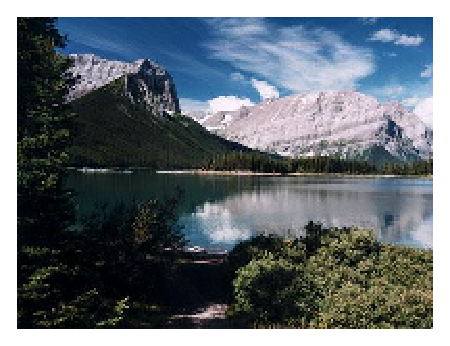
\epsfig{file=kananaskis_small.ps} \raisebox{2.5cm}{\Huge\bf~~~+~} 
\raisebox{0mm}{\epsfig{file=scratchBDD.ps, height=5.3cm, width=3.5cm}}
}}

\vfill

\newpage

\pagenumbering{roman}

\section*{Preface}


The development of {\tt HolBddLib} has gone through two phases.  The
first phase consisted in experiments with different ways of linking
higher order logic (HOL) terms to binary decision diagrams (BDDs).
These are described in the paper {\it Reachability programming in
HOL98 using BDDs\/} \cite{tphols2000-Gordon}. The first release of
\t{HolBddLib}, called now Version~1, consisted of an ad hoc collection
of tools developed for these experiments.  The positive results of
Hasan Amjad \cite{Amjad:TPHOLs2001} have lead us to adopt an
approaches based on a protected type of `BDD representation
judgements', analogous to the LCF protected type of theorems.  The goal
of \t{HolBddLib} Version~2, described here, is to use a kernel of representation
judgement rules to provide core infrastructure for building
`fully-expansive' or `LCF-style' combinations of HOL theorem proving
and BDD-based symbolic calculation algorithms, like model checkers.

Version~1 of {\tt{HolBddLib}} was more elaborate than Version~2
because it mixed together code from a number of experiments.
Version~2 narrows attention to the representation judgement approach,
and provides a fixed set of `inference rules' that link terms to
BDDs. All higher level tools, such as model checkers, are programmed
in ML as `derived rules'.

The primitive inference rules for representation judgements are in the structure
{\tt{PrimitiveBddRules}}. A few example derived rules are in the
structure {\tt{DerivedBddRules}}. Currently the only derived rules are
ones to compute reachable states and find sequences of transitions to
states with given properties.  It is hoped to soon add a module for
checking properties expressed in the modal $\mu$-calculus (and hence CTL).

In {\tt{HolBddLib}} Version~1 there was a function, called
{\texttt{termToBdd}}, that tried to represent a \HOL{} term as a BDD
using a dynamically extendable global table mapping \HOL{} terms to
BDDs.  $\t{TermToBdd}$ constructed the BDD of a term $t$ using any
BDDs of subterms of $t$ that were stored in the global table.
{\tt{HolBddLib}} Version~2 has jettisoned this imperative style based
on a global BDD state in favour of a purely functional rules. Some of
the ideas of BDD tables are likely to return in the future, but as
contexts, similar to HOL simpsets, that are passed functionally,
rather than as a single global state held in references.

{\tt{HolBddLib}} Version~1 only supported a single variable
ordering, held in a global variable map. In Version~2, each
representation judgement carries its own variable ordering, so that local
scopes are possible. For convenience, {\tt{DerivedBddRules}}
provides a way of storing a default variable ordering in a global
variable, but this is just a derived facility, not part of the kernel.

{\tt{HolBddLib}} Version~2 adds assumptions to representation judgements
analogous to assumptions of HOL theorems. This enables
Coudert, Berthet and Madre simplification to be represented as a primitive
rule (see the rule \t{BddSimplify} in 
Section~\ref{term-bdd-rules}). 
It also allows the term part
of a representation judgements to be simplified using equations with assumptions
(see the rule \t{BddEqMp} in Section~\ref{BddEqMp}).

{\tt HolBddLib} uses J{\o}rn Lind-Nielsen's \Buddy{} package as a BDD
engine. The interface from \Buddy{} to Moscow ML, called \Muddy, is
due to Ken Friis Larsen and Jakob Lichtenberg, and is described in Part~\ref{muddy}.
{\tt HolBddLib} is built on top of \Muddy{} and
is described in Part~\ref{HolBddLib}.

Some of the material in this document derives from University of
Cambridge Computer Laboratory Technical Report No.~481, December 1999,
by Mike Gordon and Ken Friis Larsen \cite{GordonLarsen}. Although this
report has examples that might be of tutorial use, it has much
obsolete material and methodology deriving for early experiments
pre-dating the release of {\tt HolBddLib} Version~1.


\subsection*{History and related work\footnote{Adapted from 
{\it Reachability programming in HOL using BDDs}
\cite{tphols2000-Gordon}}}\label{related}

The Voss system \cite{SegerVoss} has strongly influenced
the ideas described here. Voss consists of a lazy
ML-like functional language, called FL, with BDDs as a built-in datatype.
Quantified boolean formulae can be input and are parsed to BDDs.
The normal boolean operations $\neg$, $\wedge$, $\vee$, $\equiv$,
$\forall$, $\exists$ are interpreted as BDD operations.  
Algorithms for model checking are easily programmed.

Joyce and Seger interfaced an early HOL system (HOL88) to Voss and in
a pioneering paper showed how to verify complex systems by a
combination of theorem proving deduction and symbolic trajectory
evaluation (STE) \cite{JoyceSeger}. The HOL-Voss system integrates HOL88
deduction with BDD computations.  BDD tools are programmed in FL and
can then be invoked by HOL-Voss tactics, which can make external
calls into the Voss system, passing subgoals via a translation between
the HOL88 and Voss term representations.

In later work Lee, Seger and Greenstreet \cite{LeeGreenstreetSeger}
showed how various optimised BDD algorithms could be programmed in FL.

The early experiments with HOL-Voss suggested that a lighter theorem
proving component was sufficient, since all that was really needed was
a way of combining results obtained from STE. A system based on this
idea, called VossProver, was developed by Carl Seger and his student
Scott Hazelhurst. It provides operations in FL for combining
assertions generated by Voss using proof rules corresponding to the
laws of composition of the temporal logic assertions verified by STE
\cite{hazelhurst-kropfbook-97}.  
VossProver was used to verify
impressive integer and floating-point examples (see the DAC98
paper by Aagaard, Jones and Seger \cite{aagaard-dac-98} for further
discussion and references). 

After Seger and Aagaard moved to Intel, the development of the Voss and
VossProver systems evolved into a new system called Forte.  Only partial details
of this are in the public domain
\cite{oleary-itj-99,aagaard-tphols-99}, but a key idea is that FL is
used both as a specification language and as an LCF-style
metalanguage. The connection between symbolic trajectory evaluation
and proof is obtained via a tactic {\tt{Eval\_tac}} that converts the
result of executing an FL program performing STE into a theorem in the
logic. Theorem proving in Forte is used both to split goals into
smaller subgoals that are tractable for model checking, and to
transform formulae so that they can be checked more efficiently.

The combination of \HOL{} and \Buddy{} in Version~1 of
{\tt{HolBddLib}} provides a somewhat similar programming environment
to Voss's FL (though with eager rather than lazy evaluation and no
special support for STE). \Buddy{} provides BDD operations
corresponding to $\neg$, $\wedge$, $\vee$, $\equiv$, $\forall$,
$\exists$ and the \HOL{} term parser plus \ml{termToBdd} provides a
way of using these to create BDDs from logical terms.  Voss enables
efficient computations on BDDs using functional programming. So does
\ml{HolBddLib}. However, in addition it allows FL-like BDD programming
in ML to be intimately mixed with \HOL{} deduction, so that, for
example, theorem proving tools (e.g.~simplifiers) can be directly
applied to terms to optimise them for BDD purposes (e.g.~disjunctive
partitioning).  This is in line with future developments discussed by
Joyce and Seger \cite{JoyceSeger} and it appears that the Forte system
has similar capabilities.

{\tt{HolBddLib}} Version~2 provides a less developed interactive
programming environment than Version~1. It is more oriented to
providing a clean and simple API allowing implementers to create their
own `fully-expansive' combinations of model checking and theorem
proving. Such a combination could be a Voss-like verification
platform.

\subsection*{Overview}


In the LCF approach, theorems are represented by an abstract type
whose primitive operations are the axioms and inference rules of a
logic.  Theorem proving tools are implemented by composing together
the inference rules using ML programs.

This idea can be generalised to computing valid judgements that
represent other kinds of information. In particular, consider
judgements $(a,\rho,t,b)$, where $a$ is a set of boolean terms
(assumptions) that are assumed true, $\rho$ represents a variable
order, $t$ is a boolean term all of whose free variables are boolean
and $b$ is a BDD. Such a judgement is valid if under the assumptions
$a$, the BDD representing $t$ with respect to $\rho$ is $b$, and we
will write \termbdd{a}{\rho}{t}{b} when this is the case.

The derivation of `theorems' like \termbdd{a}{\rho}{t}{b} can be viewed
as `proof' in the style of LCF by defining an abstract type \termbddty{}
whose primitive operations correspond to the BDD functions provided by \Buddy.
The type $\termbddty$ models judgements $\termbdd{a}{\rho}{t}{b}$ analogously
to the way the type $\ty{thm}$ models theorems $\vdash t$.

\t{HolBddLib} currently contains two structures: \t{PrimitiveBddRules}
which defines a protected type \termbddty and rules for generating
values of this type, and \t{DerivedBddRules} that contains derived
rules for performing simple fixed-point calculations.  There is also a
theory \t{DerivedBddRulesTheory} containing the theorems on
reachability and fixed points needed by the derived rules.

\newpage
\tableofcontents

\pagenumbering{arabic}
\newpage

\part{\Muddy}\label{muddy}

\Muddy is the Moscow
ML interface to \Buddy. It provides ML functions for constructing and
manipulating BDDs via three structures:

\begin{itemize}

\item \t{bdd} defines the ML type
\t{bdd} representing BDDs and associated operations derived from \Buddy;


\item \t{fdd} provides support for blocks of BDD variables
used to encode values representing elements of finite domains;

\item \t{bvec} provides support for Boolean vectors.

\end{itemize}

The current \HolBuddy{} system only uses \t{bdd} and so
the documentation of \t{fdd} and \t{bvec} provided here is minimal
(see Sections~\ref{fdd} and \ref{bvec} below).

\section{Initialisation, termination and tuning sessions}\label{init}

The \Buddy{} package must be initialised before any BDD operations are done.
Initialisation is done with the ML function

\begin{verbatim}
   init : int -> int -> unit
\end{verbatim}\bnind{\ml{init}}

Evaluating $\t{init}~m~n$ initialises \Buddy{} with $m$ nodes in the
nodetable and a cachesize of $n$.  
The library \t{HolBddLib} (Section~\ref{HolBddLib}) 
initialises the nodetable to 1000000 and cachesize to
be 10000. The following is a quotation from the \Buddy{} documentation \cite{BuDDy}.

\vspace*{-2mm}

{\baselineskip8pt\begin{quote}\footnotesize
Good initial values are

\smallskip

\begin{tabular}{lrr}
{\bf Example} & {\bf nodenum} & {\bf cachesize} \\
Small test examples   & 1000    & 100\\
Small examples        & 10000   & 1000 \\
Medium sized examples & 100000  & 10000\\
Large examples        & 1000000 & 10000
\end{tabular}

\smallskip

Too few nodes will only result in reduced performance and this
increases the number of garbage collections needed. If the package
needs more nodes, then it will automatically increase the size of the
node table.
\end{quote}}

The initial number of nodes is not critical for any BDD operation
as the table will be resized whenever there are too few nodes left
after a garbage collection.  But it does have some impact on the
efficiency of the operations.

The function

\begin{verbatim}
   done : unit -> unit
\end{verbatim}\bnind{\ml{done}}

frees all memory used by \Buddy{} and resets the
package to its initial state. 

The functions \t{init} and \t{done} should only be called once per session.

The function

\begin{verbatim}
   isRunning : unit -> bool
\end{verbatim}\bnind{\ml{isRunning}}

tests whether
\Buddy{} is running (i.e.~\t{init} has been called and \t{done} has not been called). It is
useful for checking if initialialisation is needed -- see Section~\ref{HolBddLib}.

The functions \t{init} and \t{done} should only be called once in a session.

Statistical information from \Buddy{} is available
using the function \t{stats}

\begin{verbatim}
   stats : unit -> {produced     : int,
                    nodenum      : int,
                    maxnodenum   : int,
                    freenodes    : int,
                    minfreenodes : int,
                    varnum       : int,
                    cachesize    : int,
                    gbcnum       : int}
\end{verbatim}\bnind{\ml{stats}}

The meaning of the values of the various named fields in the record returned by
evaluating \t{stats()} are

\medskip

\begin{tabular}{|l|l|} \hline
{\bf{Field name}}& {\bf{Meaning}}                                              \\ \hline\hline
\t{produced}     & total number of new nodes ever produced                     \\ \hline
\t{nodenum}      & currently allocated number of BDD nodes                     \\ \hline
\t{maxnodenum}   & user defined maximum number of BDD nodes                    \\ \hline
\t{freenodes}    & number of currently free BDD nodes                          \\ \hline
\t{minfreenodes} & minimum number of nodes left after a BDD garbage collection \\ \hline
\t{varnum}       & number of defined BDD variables                             \\ \hline
\t{cachesize}    & number of cache entries                                     \\ \hline
\t{gbcnum}       & number of BDD garbage collections done                      \\ \hline
\end{tabular}

\medskip

The management of the node table and internal caches can be tuned
using the following functions


\begin{verbatim}
   setMaxincrease : int -> int
   setCacheratio  : int -> int
\end{verbatim}\bnind{\ml{setMaxincrease}}\bnind{\ml{setCacheratio}}

Evaluating \t{setMaxincrease~$n$} tells \Buddy that the maximum of new nodes added
when doing an expansion of the nodetable should be $n$.  The previous maximum is returned.

Evaluating \t{setCacheratio~$n$} sets the cache ratio to $n$.  
For example, if $n$ is $4$ then the internal caches will be $\frac{1}{4}$ the size of the
nodetable.



\section{BDDs representing {\t{true}} and {\t{false}}}

The atomic BDDs representing the two truthvalues are bound to the ML
identifiers \t{TRUE} and \t{FALSE}, both of type \t{bdd}.

Functions for mapping from ML Booleans to BDDs and vice versa are, respectively

\begin{verbatim}
   fromBool : bool -> bdd
   toBool   : bdd  -> bool
\end{verbatim}\bnind{\ml{fromBool}}\bnind{\ml{toBool}}

The function \t{toBool} returns \t{true} on TRUE and \t{false} on FALSE.
It raises the exception \t{Domain} on non-atomic BDDs.

\begin{verbatim}
   equal : bdd -> bdd -> bool
\end{verbatim}\bnind{\ml{equal}}

tests the equality of two BDDs. Thus \t{TRUE} is \t{equal} to \t{fromBool(true)} and 
\t{FALSE} is \t{equal} to \t{fromBool(false)}.

\section{Variables}

In \Buddy, BDD variables are encoded as integers (type \t{int} in ML) and the BDD variable ordering
is the numerical ordering. Thus to build a BDD to represent a \HOL{} term with a
particular variable ordering it is necessary to map \HOL{} variables to
integers so that the numerical order corresponds to the desired
variable order.

The number of variables in use must be declared using

\begin{verbatim}
   setVarnum : int -> unit
\end{verbatim}\bnind{\ml{setVarnum}}

Evaluating $\t{setVarnum}~n$ declares that the $n$ variables $0$,
$1$, $\ldots$ , $n{-}1$ are available for use. The number of variables
can be increased dynamically during a session by calling \t{setVarnum}
with a larger number. The number of variables cannot be decreased
dynamically. The function

\begin{verbatim}
   getVarnum : unit -> int
\end{verbatim}\bnind{\ml{getVarnum}}

returns the number of variables in use (i.e.~the argument of the last
application of \t{setVarnum}).

The function

\begin{verbatim}
   ithvar : int -> bdd
\end{verbatim}\bnind{\ml{ithvar}}

maps an ML integer to a BDD that consists of just the variable
corresponding to the integer and

\begin{verbatim}
   nithvar : int -> bdd
\end{verbatim}\bnind{\ml{nithvar}}

maps
an integer to BDD representing the negation of the variable.

Note that evaluating $\t{ithvar}~n$ or $\t{nithvar}~n$ will raise the exception
\t{Fail} (with string argument \texttt{"Unknown variable"})
if $n$ has not been declared as in use, i.e.~if
$\t{setVarnum}~m$ has not been previously evaluated for some $m$
greater than $n$.


\section{Sets of variables and quantification}\label{varSet}

\Buddy{} provides operations on BDDs for quantifying with respect to sets
of variables. The module  \t{bdd} provides a type \t{varSet} to represent such
sets with, respectively, a constructor and two destructors:

\begin{verbatim}
   makeset : int list -> varSet
   scanset : varSet   -> int vector
   fromSet : varSet   -> bdd
\end{verbatim}\bnind{\ml{makeset}}\bnind{\ml{scanset}}\bnind{\ml{fromSet}}

The destructor \t{scanset} returns a vector of the variables in the
set and the destructor \t{fromSet} returns a BDD representing the
conjunction of the variables in the set.

The following functions quantify BDDs with respect to sets of variables:

\begin{verbatim}
   forall : varSet -> bdd -> bdd
   exist  : varSet -> bdd -> bdd
\end{verbatim}\bnind{\ml{forall}}\bnind{\ml{exist}}

\t{forall} universally quantifies a BDD and \t{exist} existentially quantify a BDD.

\section{Assignments, composition, replacement and restriction}\label{replace}

\Muddy provides a general purpose simultaneouse substitution function 
and several optimised functions for the special cases of substituting for a single variable,
renaming variables and substituting with boolean constants.

The operation \t{veccompose} performs the simultaneous substitution 
of BDDs for variables in a BDD. The argument of \t{veccompose}
is a value of type \t{composeSet}\tyind{\ml{composeSet}} 
(created with a constructor \t{composeSet})
that specifies the substitution.

\begin{verbatim}
   composeSet : (varnum * bdd) list -> composeSet
   veccompose : composeSet -> bdd -> bdd
\end{verbatim}\bnind{\ml{composeSet}}\bnind{\ml{veccompose}}

A single variable can be replaced with a BDD using

\begin{verbatim}
   compose : bdd -> bdd -> int -> bdd
\end{verbatim}\bnind{\ml{compose}}

Evaluating \t{compose~$b_1$~$b_2$~$n$} substitutes $b_2$ for the
variable $n$ in $b_1$.

Variables can be renamed using the function \t{replace} that takes
an argument of type \t{pairSet}\tyind{\ml{pairSet}} representing sets of pairs of variables
(with constructor \t{makepairSet})

\begin{verbatim}
   makepairSet : (int * int)list -> pairSet
   replace     : bdd -> pairSet -> bdd
\end{verbatim}\bnind{\ml{makepairSet}}\bnind{\ml{replace}}

Evaluating \t{makepairSet[($x_1$,$x_1'$), $\ldots$ , ($x_n$,$x_n'$)]}
creates a set of pairs specifying that $x_i'$ be substituted for $x_i$
(for $1\leq i\leq n$).  A renaming with \t{replace} will fail if it
would result in distinct variables being identified (i.e.~if the shape of the BDD would change).

BDDs can be restricted by instantiating variables to {\t{TRUE}} or
{\t{FALSE}} using the function \t{restrict} that takes
as argument a value of type \t{assignment}\tyind{\t{assignment}} 
(which has a constructor \t{assignment} and destructor \t{getAssignment}).

\begin{verbatim}
   assignment    : (int * bool)list -> assignment
   getAssignment : assignment -> (int * bool) list
   restrict      : bdd -> assignment -> bdd
\end{verbatim}\bnind{\ml{restrict}}\bnind{\ml{assignment}}\bnind{\ml{getAssignment}}

Evaluating \t{assignment[($v_1$,$t_1$), $\ldots$ , ($v_n$,$t_n$)]}
creates an assignment specifying that each $v_i$ be instantiated to
$\t{fromBool(}t_i\t{)}$ (for $1{\leq}i{\leq}n$). 


\section{Finding satisfying assignments}

An assignment satisfying a BDD can be computed via \Buddy using

\begin{verbatim}
   satone : bdd -> assignment
\end{verbatim}\bnind{\ml{makeset}}\bnind{\ml{scanset}}\bnind{\ml{fromSet}}

The exception \t{Domain} is raised if the argument to \t{satone} is unsatisfiable.

Alternatively, a model can be computed by an ML program such as:

\begin{verbatim}
   val findSat =
    let fun findSatAux bdd = 
         if bdd.equal bdd bdd.TRUE
          then []
          else
           if bdd.equal bdd bdd.FALSE
            then raise Domain
            else
             ((bdd.var bdd,true) :: findSatAux(bdd.high bdd) 
              handle Domain =>
              (bdd.var bdd, false) :: findSatAux(bdd.low bdd))
    in
     assignment o findSatAux
    end;
\end{verbatim}

The functions \t{satOne} and \t{findSat} do not necessarily find the
same satisfying assignment, if more than one exists. Also,
\t{findSat} stops when it has found enough variable bindings to
satisfy the BDD, so may not return an assignment giving values to all
the variables.

\section{Boolean operations on BDDs}\label{app}

The structure \t{bdd} introduces a type \t{bddop}
corresponding to Boolean operations on BDDs. 
The ML function

\begin{verbatim}
   apply : bdd -> bdd -> bddop -> bdd
\end{verbatim}\bnind{\ml{apply}}

applies a BDD operation to BDD values.

\Buddy{} provides functions for calculating in a single step the
result of performing a Boolean operation and then quantifying the
result with respect to several variables.

\begin{verbatim}
   appall : bdd -> bdd -> bddop -> varSet -> bdd
   appex  : bdd -> bdd -> bddop -> varSet -> bdd
\end{verbatim}\bnind{\ml{appall}}\bnind{\ml{appex}}

The function \t{appall} universally quantifies the result of the
Boolean operation and \t{appex} existentially quantifies it.

\Muddy{} provides ten operations of type \t{bddop} and for each of
these an ML infix, pre-defined using \t{apply}, of type \t{bdd~*~bdd~->~bdd}.



\begin{center}

\begin{tabular}{|l||l|l|} \hline
\t{bddop}\bnind{\ml{bddop}} & \t{bdd~*~bdd~->~bdd} & Result of applying to $(b_1,b_2)$\\ \hline\hline
\t{And}\bnind{\ml{And}} & \t{AND} & $b_1\wedge b_2$ \\ \hline
\t{Nand}\bnind{\ml{Nand}} & \t{NAND} & $\neg(b_1\wedge b_2)$ \\ \hline
\t{Or}\bnind{\ml{Or}}  & \t{OR} & $b_1\vee b_2$ \\ \hline
\t{Nor}\bnind{\ml{Nor}} & \t{NOR} & $\neg(b_1\vee b_2)$ \\ \hline
\t{Biimp}\bnind{\ml{Biimp}} & \t{BIIMP} & $b_1= b_2$ \\ \hline
\t{Xor}\bnind{\ml{Xor}} & \t{XOR} & $\neg(b_1=b_2)$ \\ \hline
\t{Imp}\bnind{\ml{Imp}} & \t{IMP} & $b_1\imp b_2$ \\ \hline
\t{Invimp}\bnind{\ml{Invimp}} & \t{INVIMP} & $b_2\imp b_1$ \\ \hline
\t{Lessth}\bnind{\ml{Lessth}} & \t{LESSTH} & $\neg b_1\wedge b_2$ \\ \hline
\t{Diff}\bnind{\ml{Diff}} & \t{DIFF} & $b_1\wedge \neg b_2$ \\ \hline
\end{tabular}\label{bddops}

\end{center}

\Muddy{} also provides a unary negation operator and ternary conditional operator.

\begin{verbatim}
   NOT : bdd -> bdd
   ITE :  bdd -> bdd -> bdd -> bdd
\end{verbatim}\bnind{\ml{NOT}}\bnind{\ml{ITE}}

$\t{NOT}~b$ is the BDD corresponding to  `$\neg b$' and $\t{ITE}~b~b_1~b_2$ is the BDD corresponding
to `$if~b~then~b_1~else~b_2$'.




\section{Inspecting and counting nodes and states}

The integer labelling a BDD node and the BDDs corresponding to the high
(i.e.~{\t{true}}) and low (i.e.~{\t{false}}) nodes are obtained,
respectively, with

\begin{verbatim}
   var  : bdd -> int
   high : bdd -> bdd
   low  : bdd -> bdd
\end{verbatim}\bnind{\ml{var}}\bnind{\ml{high}}\bnind{\ml{low}}

Thus if $b$ is the BDD of ``${\it{if}}~x~{\it{then}}~t_1~{\it{else}}~t_2$''
then $\t{var}~b$ will return the number representing variable $x$,
$\t{high}~b$ will return the BDD of $t_1$ and $\t{low}~b$ will return
the BDD of $t_2$.

Note that \t{var}, \t{high} and \t{low} raise an exception if applied
to \t{TRUE} or \t{FALSE}.

The entire \Buddy{} node table of a BDD can be copied into ML using

\begin{verbatim}
   nodetable : bdd -> int * (int * int * int)vector
\end{verbatim}\bnind{\ml{nodetable}}

The integer returned as the first component of the pair is a pointer
(starting from 0) into the second component, a vector of node
descriptors. This pointer points to the root node. Each node
descriptor is a triple of integers $(v,l,h)$, where $v$ is the node
label (i.e.~a number representing a variable), $l$ points to the low
({\t{false}}) node in the vector and $h$ points to the high
({\t{true}}) node. The first two nodes in the vector are special:
they represent {\t{true}} and {\t{false}}, respectively, and arbitrarily have
the structure $(0,0,0)$.

The number of nodes in a BDD is computed by the function

\begin{verbatim}
   nodecount : bdd -> int
\end{verbatim}\bnind{\ml{nodecount}}

This could be defined by

\begin{verbatim}
   fun nodecount bdd = Vector.length(snd(nodetable bdd));
\end{verbatim}

However, \t{nodecount} defined this way is likely to run out of space
on large BDDs (since it involves copying the argument BDD from
\Buddy's representation into an ML vector).  Thus the ML function
provided by \Muddy{} invokes \Buddy's \t{nodecount} function directly
and so is space-efficient.

The number of assignments {\it to all variables in use in the current
session\/} that satisfy a BDD (i.e.~make it true) is given by the ML
function

\begin{verbatim}
   satcount : bdd -> real
\end{verbatim}\bnind{\ml{satcount}}

The answer is exact until the result is too big to be represented as a
Moscow ML integer. Real numbers are used so that results can be
returned when this happens.

The function

\begin{verbatim}
   support : bdd -> varSet
\end{verbatim}\bnind{\ml{support}}

gives the variables that a BDD depends on. 

An application is to define
a function that counts the number of valuations of a BDD using
\t{satcount}.

\begin{verbatim}
   statecount : bdd -> real
\end{verbatim}\bnind{\ml{statecount}}

The
definition of \t{statecount} is

\begin{verbatim}
fun statecount bdd =
 let val sat    = satcount bdd
     val total  = Real.fromInt(getVarnum())
     val sup    = scanset(support bdd)
     val numsup = Real.fromInt(Vector.length sup)
     val free   = total - numsup
 in 
  if equal bdd TRUE 
   then 0.0
   else sat / Math.pow(2.0, free)
 end
\end{verbatim}

If a BDD is representing a set of states, then \t{statecount} gives
the number of states in the set (hence the name).


\section{Coudert, Berthet \& Madre simplification}

The ML function

\begin{verbatim}
   simplify : bdd -> bdd -> bdd
\end{verbatim}\bnind{\ml{simplify}}

simplifies its second argument under the assumption that the first
argument is true. Thus evaluating
\t{simplify~$b_1$~$b_2$} results in a BDD $b_2'$, hopefully simpler than $b_2$, such that
$b_1 \Imp (b_2 = b_2')$ or, equivalently, \mbox{$b_1 \wedge b_2 = b_1 \wedge b_2'$}.
More precisely,
the relationship between $b_1$, $b_2$ and $b_2'$ is that
the BDD \t{IMP($b_1$,BIIMP($b_2$,$b_2'$))} is the BDD \t{TRUE}
(or, equivalently, that \t{AND($b_1$,$b_2$)} and \t{AND($b_1$,$b_2'$)}
are \t{equal}, i.e.~the same BDD).

For more details see Henrik Reif Andersen's lecture
notes on BDDs \cite{HenrikNotes}, where
the algorithm underlying \t{simplify} is described and attributed to a paper by
Coudert, Berthet and Madre \cite{CoudertBerthetMadre}.

It is not clear how to provide a BDD representation judgement rule
corresponding to \t{simplify}.

\section{Saving, hashing and printing BDDs}

BDDs can be saved on disk with the functions

\begin{verbatim}
   bddSave : string -> bdd -> unit
   bddLoad : string -> bdd
\end{verbatim}\bnind{\ml{bddSave}}\bnind{\ml{bddLoad}}

The string argument is a file name.

\Buddy{} provides two ways of printing BDDs: (i) as the set of paths from
the root node to the {\it{true}} node and (ii) to the format used by
the \t{dot} graph drawing
program\footnote{\tt{http://www.research.att.com/sw/tools/graphviz/}}.

The function

\begin{verbatim}
   hash : bdd -> int
\end{verbatim}\bnind{\ml{hash}}

hashes a bdd to an integer.

The functions for printing BDDs are;

\begin{verbatim}
   printset   : bdd -> unit
   printdot   : bdd -> unit
   fnprintset : string -> bdd -> unit
   fnprintdot : string -> bdd -> unit
\end{verbatim}\bnind{\ml{printset}}\bnind{\ml{printdot}}\bnind{\ml{fnprintset}}\bnind{\ml{fnprintdot}}

\t{printset} and \t{printdot} print to standard output, whilst
\t{fnprintset} and \t{fnprintdot} print to a file with the supplied
name.

\t{printset} and \t{fnprintset} print out a sequence of paths, each one having the form

\smallskip

~$\t{}<m_0\t{:}n_0\t{,} \ldots \t{,} m_l\t{:}n_l\t{>}$

\smallskip

where the $n_0$, $\ldots$ , $n_l$ after the colon (\t{:}) are \t{0} or
\t{1} and indicate that the next node in the path is reached by
following the low ({\t{false}}) or high ({\t{true}}) pointer,
respectively. 

For
example, evaluating

\smallskip
~\t{printset~(AND(ithvar~0,~OR(ithvar~1,~NOT(ithvar~2))))}
\smallskip

results in

\smallskip
~\t{<0:1,~1:0,~2:0><0:1,~1:1>}
\smallskip

which is best understood by looking at the diagram of the BDD drawn by
\t{dot} that appears below.

To illustrate printing to \t{dot} format,  the same BDD can be
printed to a file \t{ex} by evaluating

\smallskip
~\t{fnprintdot~"ex"~(AND(ithvar~0,~OR(ithvar~1,~NOT(ithvar~2))))}
\smallskip

executing ~\t{dot~-Tps~ex~>~ex.ps} (in Unix) results in
the following Postscript diagram of a BDD

\begin{center}
\epsfig{file=ex.ps, height=5cm, width=3cm} 
\end{center}

\section{Dynamic variable reordering}

\Buddy{} provides functions for dynamic variable reordering using a variety of methods.
See the \Buddy{} documentation \cite{BuDDy} for further details. The dynamic reordering
types and functions provided in ML via \Muddy{} are in the structure \t{bdd} and are

{\tiny\begin{verbatim}
    eqtype fixed
    FIXED            : fixed
    FREE             : fixed

    addvarblock      : varnum -> varnum -> fixed -> unit
    clrvarblocks     : unit -> unit

    eqtype method
    WIN2             : method
    WIN2ITE          : method
    SIFT             : method
    SIFTITE          : method
    RANDOM           : method
    REORDER_NONE     : method

    reorder          : method -> unit
    autoReorder      : method -> method
    autoReorderTimes : method -> int -> method

    getMethod        : unit -> method
    getTimes         : unit -> int

    disableReorder   : unit -> unit
    enableReorder    : unit -> unit

    varToLevel       : varnum -> int
    varAtLevel       : int -> varnum
\end{verbatim}}

\section{The \Muddy{} structure \t{fdd}}\label{fdd}

The structure \t{fdd} provides functions for manipulating values of finite domains.
Functions are provided to allocate blocks of BDD variables to represent integer values instead
of only Booleans.

Encoding is done with the least significant bits first in the BDD ordering. For example, if variables
$v_0, v_1, v_2, v_3$ are used to encode $12$, then the encoding would yield
$v_0=0$, $v_1=0$, $v_2=1$ and $v_3=1$.

See the \Buddy{} documentation \cite{BuDDy} for further details. See the ML structure \t{fdd}
for the \Buddy{} facilities provides in ML via \Muddy:

{\tiny\begin{verbatim}
   type fddvar

   extDomain  : int list -> fddvar list
   clearAll   : unit -> unit
   domainNum  : unit -> int
   domainSize : fddvar -> int
   varNum     : fddvar -> int
   vars       : fddvar -> bdd.varnum list
   ithSet     : fddvar -> bdd.varSet
   domain     : fddvar -> bdd.bdd
   setPairs   : (fddvar * fddvar) list -> bdd.pairSet
\end{verbatim}}

\section{The \Muddy{} structure \t{bvec}}\label{bvec}

The structure \t{bvec} provides tools for encoding integers as arrays
of BDDs, where each BDD represents one bit of an expression.

See the \Buddy{} documentation \cite{BuDDy} for further details. See the ML structure \t{bvec}
for the \Buddy{} facilities provides in ML via \Muddy{}.

{\tiny
\begin{verbatim}
   type bvec

   bvectrue    : fdd.precision -> bvec 
   bvecfalse   : fdd.precision -> bvec 
   con         : fdd.precision -> int -> bvec
   var         : fdd.precision -> bdd.varnum -> int -> bvec
   varfdd      : fdd.fddvar -> bvec

   coerce      : fdd.precision -> bvec -> bvec

   isConst     : bvec -> bool
   getConst    : bvec -> int
   lookupConst : bvec -> int option

   add         : bvec * bvec -> bvec
   sub         : bvec * bvec -> bvec
   mul         : bvec * bvec -> bvec
   mulfixed    : bvec * int -> bvec
   div         : bvec * bvec -> bvec * bvec
   divfixed    : bvec * int -> bvec * bvec
   divi        : bvec * bvec -> bvec
   divifixed   : bvec * int -> bvec

   modu        : bvec * bvec -> bvec
   modufixed   : bvec * int -> bvec
   shl         : bvec -> bvec -> bdd.bdd -> bvec
   shlfixed    : bvec -> int -> bdd.bdd -> bvec
   shr         : bvec -> bvec -> bdd.bdd -> bvec
   shrfixed    : bvec -> int -> bdd.bdd -> bvec

   lth         : bvec * bvec -> bdd.bdd
   lte         : bvec * bvec -> bdd.bdd
   gth         : bvec * bvec -> bdd.bdd
   gte         : bvec * bvec -> bdd.bdd
   equ         : bvec * bvec -> bdd.bdd
   neq         : bvec * bvec -> bdd.bdd
\end{verbatim}}

\section{Storage allocation and garbage collection}
\label{sec:technical-details}

The heart of the \Muddy package is mostly stub code that mirrors the
\Buddy API and takes care of translating C values into SML values and
vice versa.

The most tricky part is to make the \mosml garbage collector cooperate
with the \Buddy garbage collector (we don't want either collector to
try to collect the other's garbage).  The cooperation is done by using
the \emph{finalized values} facility of the \mosml runtime system.
That is, whenever a \texttt{bdd} value is returned from the \Buddy
library, \Muddy register it as an external root (via
\verb+bdd_addref+) and wraps it into a finalized value.  

A finalized value, in the \mosml runtime system, is a pair where the
first component is the \emph{destructor} (a function pointer) and the
second component is the \emph{data} (typicaly a pointer).  When the
\mosml collector collect a finalized value it apply the destructor on
the data.  In the case of the \Muddy package the destructor is
\verb+bdd_delref+ and the data is the node-index returned by \Buddy.

Output showing the activation of the \Buddy garbage collector can be generated
using the function

\begin{verbatim}
   verbosegc : (string * string) option -> unit
\end{verbatim}\bnind{\ml{verbosegc}}

Evaluating \t{verbosegc(SOME($pregc$,$postgc$))} instructs BuDDy to print
$pregc$ when a BuDDy GC is initiated and print $postgc$ when the
\Buddy GC is completed.

\newpage

\part{Description of \t{HolBddLib}}\label{HolBddLib}

\t{HolBddLib} consists of four modules

\begin{enumerate}
\item \t{Varmap} defines the ML type \t{varmap} that represents mappings,
often denoted by $\rho$,
from HOL variables to BDD variables;

\item \t{PrimitiveBddRules} defines the protected type \termbddty
representing BDD representation judgements \termbdd{a}{\rho}{t}{b}
that assert that under assumptions $a$, term $t$ is represented by BDD $b$ with respect to
varmap $\rho$;

\item \t{DerivedBddRules} defines some derived rules for computing
the representation of the reachable states of a transition system,
and also for finding shortest paths to states  satisfying a given property;

\item \t{DerivedBddRulesTheory} contains HOL reachability and fixedpoint theorems needed
for the derived rules in  \t{DerivedBddRules}.


\end{enumerate}


Executing

\vspace*{-2mm}

\begin{verbatim}
   load "HolBddLib";
\end{verbatim}

\vspace*{-2mm}

loades these four modules and
initialises \Buddy{} with a nodesize of 1000000
and cachesize of 10000.  

If you want to perform your own \Buddy{} initialisation with different
values, then instead of loading \t{HolBddLib}, load \t{bdd} and then
call \t{bdd.init} with the parameters you want (see
Section~\ref{init}).  \t{PrimitiveBddRulesTheory} and/or
\t{DerivedBddRulesTheory} etc.~can  then be loaded.

\section{The structure \ml{Varmap}}\label{Varmap}

The type \t{varmap} is defined by

\vspace*{-2mm}

\begin{verbatim}
   type varmap = (string, int) Binarymap.dict
\end{verbatim}

\vspace*{-2mm}

Strings are the names of HOL boolean variables and the integers associated with them
are the corresponding BDD variables.

\newpage

The following operations and predicates on varmaps are provided:

\begin{verbatim}
   empty   : varmap
   insert  : string * int -> varmap -> varmap
   remove  : string -> varmap -> varmap
   peek    : varmap -> string -> int option
   dest    : varmap -> (string * int) list
   eq      : varmap * varmap -> bool
   size    : varmap -> int
   extends : varmap -> varmap -> bool
\end{verbatim}

with the following semantics

\bigskip

\begin{tabular}{|l|l|} \hline
\t{Varmap.empty} &    the empty varmap \\ \hline
\t{Varmap.insert} &   add an entry \\ \hline
\t{Varmap.remove} &   delete an entry for a variable \\ \hline
\t{Varmap.peek} &     lookup the value of a variable \\ \hline
\t{Varmap.dest} &     convert to a list of pairs \\ \hline
\t{Varmap.eq} &       pointer equality of varmaps ({\it not} general equality) \\ \hline
\t{Varmap.size} &     number of entries \\ \hline
\t{Varmap.extends} &  test if first argument included in second argument\\ \hline
\end{tabular}

\section{The structure \t{PrimitiveBddRules}}\label{PrimitiveBddRules}


The structure \ml{PrimitiveBddRules} defines the type \termbddty{} by

\vspace*{-2mm}

\begin{verbatim}
   type assums = term HOLset.set;
   datatype term_bdd = TermBdd of assums * varmap * term * bdd;
\end{verbatim}

\vspace*{-2mm}

The constructor \t{TermBdd} is not exported, so the only way to construct
values of type \termbddty is using the following inference rules
(which are described in more detrail in the rest of this section).

{\footnotesize\begin{verbatim}
   BddExtendVarmap           : term_bdd->varmap->term_bdd
   BddFreevarsContractVarmap : term->term_bdd->term_bdd
   BddSupportContractVarmap  : term->term_bdd->term_bdd
   BddVar                    : bool->varmap->term->term_bdd
   BddCon                    : bool->varmap->term_bdd
   BddNot                    : term_bdd->term_bdd
   BddIte                    : term_bdd*term_bdd*term_bdd->term_bdd
   BddOp                     : bddop*term_bdd*term_bdd->term_bdd
   BddForall                 : term list->term_bdd->term_bdd
   BddExists                 : term list->term_bdd->term_bdd
   BddAppall                 : term list->bddop*term_bdd*term_bdd->term_bdd
   BddAppex                  : term list->bddop*term_bdd*term_bdd->term_bdd
   BddCompose                : term_bdd*term_bdd->term_bdd->term_bdd
   BddListCompose            : (term_bdd*term_bdd)list->term_bdd->term_bdd
   BddRestrict               : (term_bdd*term_bdd)list->term_bdd->term_bdd
   BddReplace                : (term_bdd*term_bdd)list->term_bdd->term_bdd
   BddEqMp                   : thm->term_bdd->term_bdd
   BddSimplify               : term_bdd*term_bdd->term_bdd
\end{verbatim}}

Destructor functions \t{dest\_term\_bdd}, \t{getAssums} \t{getVarmap}, \t{getTerm}
and \t{getBdd} for values of type \termbddty are described in Section~\ref{misc}

There is also a single oracle function
\t{BddThmOracle} that derives the HOL theorem $a \vdash t$
from the representation judgement \termbdd{a}{\rho}{t}{\ml{TRUE}}
(details are in Section~\ref{oracle}).

\subsection{Rules for generating representation judgements}\label{term-bdd-rules}

The notation $a_1 \cup a_2$ denotes the union of $a_1$ and $a_2$ 
Assumptions of
representation judgements are identified up to $\alpha$-conversion (as
are assumptions of HOL theorems).
The implementation is $a_1 \cup a_2~=~\t{HOLset.union}~a_1~a_2$. 
The empty set of assumptions is denoted by \emptyass, a set of
assumptions containing terms $t_1, \ldots ,t_n$ is denoted by
$\setass{t_1, \ldots ,t_n}$  and 
$\termbdd{\emptyass}{\rho}{t}{b}$ is abbreviated to
$\termbdd{}{\rho}{t}{b}$.


\subsubsection*{Extending and contracting the varmap}

\newsavebox\BddExtendVarmap
\begin{lrbox}\BddExtendVarmap
\begin{minipage}{\minipagewidth}

\begin{footnotesize}
{\verb+BddExtendVarmap : term_bdd -> varmap -> term_bdd +}
\end{footnotesize}
\vspace*{-3mm}

\noindent \rule\minipagewidth{0.1pt}

\vspace*{-2mm}

$$\begin{array}{c}
\termbdd{a}{\rho_1}{t}{b} \qquad {\footnotesize\t{Varmap.extends}}~\rho_1~\rho_2
\\ \hline
\termbdd{a}{\rho_2}{t}{b}
\end{array}$$

\noindent \rule\minipagewidth{0.1pt}

\begin{footnotesize}
Raises \t{BddExtendVarmapError} if $\rho_2$ doesn not extend $\rho_1$
\end{footnotesize}
\end{minipage}
\end{lrbox}
\fbox{\usebox{\BddExtendVarmap}}

\bigskip

\newsavebox\BddFreevarsContractVarmap
\begin{lrbox}\BddFreevarsContractVarmap
\begin{minipage}{\minipagewidth}

\begin{footnotesize}
{\verb+BddFreevarsContractVarmap : term -> term_bdd -> term_bdd +}
\end{footnotesize}
\vspace*{-3mm}

\noindent \rule\minipagewidth{0.1pt}

\vspace*{-2mm}

$$\begin{array}{c}
\termbdd{a}{\rho}{t}{b} \qquad \mbox{$v$ not free in $t$}
\\ \hline
\termbdd{a}{({\footnotesize{\texttt{Varmap.remove~"}}}v{\footnotesize{\texttt{"}}}~\rho)}{t}{b}
\end{array}$$

\noindent \rule\minipagewidth{0.1pt}

\begin{footnotesize}
Raises \t{BddFreevarsContractVarmapError} if $v$ not free in $t$
\end{footnotesize}
\end{minipage}
\end{lrbox}
\fbox{\usebox{\BddFreevarsContractVarmap}}



\bigskip

\newsavebox\BddSupportContractVarmap
\begin{lrbox}\BddSupportContractVarmap
\begin{minipage}{\minipagewidth}

\begin{footnotesize}
{\verb+BddSupportContractVarmap : term -> term_bdd -> term_bdd +}
\end{footnotesize}
\vspace*{-3mm}

\noindent \rule\minipagewidth{0.1pt}

\vspace*{-2mm}

$$\begin{array}{c}
\termbdd{a}{\rho}{t}{b} \qquad \mbox{$\rho(v)$ does occur in $b$}
\\ \hline
\termbdd{a}{({\footnotesize{\texttt{Varmap.remove~"}}}v{\footnotesize{\texttt{"}}}~\rho)}{t}{b}
\end{array}$$

\noindent \rule\minipagewidth{0.1pt}

\begin{footnotesize}
Raises \t{BddSupportContractVarmapError} if $\rho(v)$ not in the support of $b$
\end{footnotesize}
\end{minipage}
\end{lrbox}
\fbox{\usebox{\BddSupportContractVarmap}}


\subsubsection*{Variables and constants}

\newsavebox\BddVar
\begin{lrbox}\BddVar
\begin{minipage}{\minipagewidth}

\begin{footnotesize}
{\verb+BddVar : bool -> varmap -> term -> term_bdd  +}
\end{footnotesize}
\vspace*{-3mm}

\noindent \rule\minipagewidth{0.1pt}

\vspace*{-2mm}

$$\begin{array}{c}
\begin{array}{c}
\rho(v)=n
\\ \hline
\termbdd{}{\rho}{v}{{\footnotesize\t{ithvar}}~n}
\end{array} ~\footnotesize{\t{BddVar~true}}

\\[8mm]

\begin{array}{c}
\rho(v)=n
\\ \hline
\termbdd{}{\rho}{v}{{\footnotesize\t{nithvar}}~n}
\end{array}~ {\footnotesize\t{BddVar~false}}

\end{array}$$

\noindent \rule\minipagewidth{0.1pt}

\begin{footnotesize}
Raises \t{BddVarError} if $v$ not in the domain of $\rho$
\end{footnotesize}
\end{minipage}
\end{lrbox}
\fbox{\usebox{\BddVar}}

\bigskip

\newsavebox\BddCon
\begin{lrbox}\BddCon
\begin{minipage}{\minipagewidth}

\begin{footnotesize}
{\verb+BddCon : bool -> varmap -> term_bdd  +}
\end{footnotesize}
\vspace*{-3mm}

\noindent \rule\minipagewidth{0.1pt}

\vspace*{-2mm}

$$\begin{array}{c}
\begin{array}{c}

\\ \hline
\termbdd{}{\rho}{{\footnotesize\t{T}}}{{\footnotesize\t{TRUE}}}
\end{array} ~\footnotesize{\t{BddCon~true}}

\\[8mm]

\begin{array}{c}
\\ \hline
\termbdd{}{\rho}{{\footnotesize\t{F}}}{{\footnotesize\t{FALSE}}~n}
\end{array}~ {\footnotesize\t{BddCon~false}}

\end{array}$$

\noindent \rule\minipagewidth{0.1pt}

\begin{footnotesize}
Always succeeds
\end{footnotesize}
\end{minipage}
\end{lrbox}
\fbox{\usebox{\BddCon}}

\subsubsection*{Boolean operations}



\newsavebox\BddNot
\begin{lrbox}\BddNot
\begin{minipage}{\minipagewidth}

\begin{footnotesize}
{\verb+BddNot : term_bdd -> term_bdd +}
\end{footnotesize}
\vspace*{-3mm}

\noindent \rule\minipagewidth{0.1pt}

\vspace*{-2mm}

$$\begin{array}{c}
\termbdd{a}{\rho}{t}{b}
\\ \hline
\termbdd{a}{\rho}{\neg t}{{\footnotesize\t{NOT}}~b}
\end{array}$$

\noindent \rule\minipagewidth{0.1pt}

\begin{footnotesize}
Always succeeds
\end{footnotesize}
\end{minipage}
\end{lrbox}
\fbox{\usebox{\BddNot}}

\bigskip

\newsavebox\BddIte
\begin{lrbox}\BddIte
\begin{minipage}{\minipagewidth}

\begin{footnotesize}
{\verb+BddIte : term_bdd * term_bdd * term_bdd -> term_bdd +}
\end{footnotesize}
\vspace*{-3mm}

\noindent \rule\minipagewidth{0.1pt}

\vspace*{-2mm}

$$\begin{array}{c}
\termbdd{a}{\rho}{t}{b} \qquad \termbdd{a_1}{\rho}{t_1}{b_1} \qquad \termbdd{a_2}{\rho}{t_2}{b_2}
\\ \hline
\termbdd{a \cup a_1 \cup a_2}{\rho}{\mbox{\footnotesize\t{(if~$t$~then~$t_1$~else~$t_2$)}}}{{\footnotesize\t{ITE}}~b~b_1~b_2}
\end{array}$$

\noindent \rule\minipagewidth{0.1pt}

\begin{footnotesize}
Raises {\footnotesize\t{BddIteError}} if the varmaps of the hypotheses are not all 
pointer equal
\end{footnotesize}
\end{minipage}
\end{lrbox}
\fbox{\usebox{\BddIte}}


\bigskip

\newsavebox\BddOp
\begin{lrbox}\BddOp
\begin{minipage}{\minipagewidth}

\begin{footnotesize}
{\verb+BddOp : bddop * term_bdd * term_bdd -> term_bdd +}
\end{footnotesize}
\vspace*{-3mm}

\noindent \rule\minipagewidth{0.1pt}

\vspace*{-2mm}

$$\begin{array}{c}
\termbdd{a_1}{\rho}{t_1}{b_1} \qquad \termbdd{a_2}{\rho}{t_2}{b_2}
\\ \hline
\termbdd{a_1\cup a_2}{\rho}{{\footnotesize\t{(termApply}}~t_1~t_2~bddop{\footnotesize\t{)}}}{{\footnotesize\t{apply}}~b_1~b_2~bddop}
\end{array}$$

\noindent \rule\minipagewidth{0.1pt}

\begin{footnotesize}
\t{termApply~$t_1$~$t_2$~$bddop$} applies
the HOL operation
corresponding to the \Buddy BDD operation $bddop$ to terms $t_1$ and $t_2$
(see Section~\ref{misc}). The exception 
{\footnotesize\t{BddOpError}} is raised if the varmaps of the hypotheses are not pointer equal
\end{footnotesize}
\end{minipage}
\end{lrbox}
\fbox{\usebox{\BddOp}}


\subsubsection*{Quantification}

\newsavebox\BddForall
\begin{lrbox}\BddForall
\begin{minipage}{\minipagewidth}

\begin{footnotesize}
{\verb+BddForall : term list -> term_bdd -> term_bdd +}
\end{footnotesize}
\vspace*{-3mm}

\noindent \rule\minipagewidth{0.1pt}

\vspace*{-2mm}

$$\begin{array}{c}
\termbdd{a}{\rho}{t}{b} \qquad \rho(v_1)=n_1,~ $\ldots$~,~ \rho(v_i)=n_i
\\ \hline
\termbdd{a}{\rho}{({\footnotesize\forall} v_1~\cdots~v_i.~t)}%
{{\footnotesize\t{forall~(makeset[}}n_1,\ldots,n_i{\footnotesize\t{])}}~b}
\end{array}$$

\noindent \rule\minipagewidth{0.1pt}

\begin{footnotesize}
Raises \t{BddForallError} if any of the terms in the term list argument
are not boolean variables in the domain of $\rho$,
or occur free in any assumption
\end{footnotesize}
\end{minipage}
\end{lrbox}
\fbox{\usebox{\BddForall}}

\bigskip


\newsavebox\BddExists
\begin{lrbox}\BddExists
\begin{minipage}{\minipagewidth}

\begin{footnotesize}
{\verb+BddExists : term list -> term_bdd -> term_bdd +}
\end{footnotesize}
\vspace*{-3mm}

\noindent \rule\minipagewidth{0.1pt}

\vspace*{-2mm}

$$\begin{array}{c}
\termbdd{a}{\rho}{t}{b} \qquad \rho(v_1)=n_1,~ $\ldots$~,~ \rho(v_i)=n_i
\\ \hline
\termbdd{a}{\rho}{({\footnotesize\exists} v_1~\cdots~v_i.~t)}%
{{\footnotesize\t{exist~(makeset[}}n_1,\ldots,n_i{\footnotesize\t{])}}~b}
\end{array}$$

\noindent \rule\minipagewidth{0.1pt}

\begin{footnotesize}
Raises \t{BddExistsError} if any of the terms in the term list argument
are not boolean variables in the domain of $\rho$,
or occur free in any assumption
\end{footnotesize}
\end{minipage}
\end{lrbox}
\fbox{\usebox{\BddExists}}

\bigskip


\newsavebox\BddAppall
\begin{lrbox}\BddAppall
\begin{minipage}{\minipagewidth}

\begin{footnotesize}
{\verb+BddAppall : term list -> bddop * term_bdd * term_bdd -> term_bdd+}
\end{footnotesize}
\vspace*{-3mm}

\noindent \rule\minipagewidth{0.1pt}

\vspace*{-2mm}

$$\begin{array}{c}
\termbdd{a_1}{\rho}{t_1}{b_1} \qquad \termbdd{a_2}{\rho}{t_2}{b_2} \qquad \rho(v_1)=n_1,~ $\ldots$~,~ \rho(v_i)=n_i
\\ \hline
\begin{array}{l}
{a_1 \cup a_2}%
~{\rho}%
~{({\footnotesize\forall} v_1~\cdots~v_i.~%
{\footnotesize\t{termApply}}~t_1~t_2~bddop)}\\
\mapsto\\
{{\footnotesize\t{appall}}~b_1~b_2~bddop~%
{\footnotesize\t{(makeset[}}n_1,\ldots,n_i{\footnotesize\t{])}}~b}
\end{array}
\end{array}$$

\noindent \rule\minipagewidth{0.1pt}

\begin{footnotesize}
Raises \t{BddAppallError} if the varmaps in the hypotheses are not pointer equal, or
if any of the terms in the term list argument
are not boolean variables in the domain of $\rho$,
or occur free in any assumption
\end{footnotesize}
\end{minipage}
\end{lrbox}
\fbox{\usebox{\BddAppall}}


\bigskip


\newsavebox\BddAppex
\begin{lrbox}\BddAppex
\begin{minipage}{\minipagewidth}

\begin{footnotesize}
{\verb+BddAppex : term list -> bddop * term_bdd * term_bdd -> term_bdd+}
\end{footnotesize}
\vspace*{-3mm}

\noindent \rule\minipagewidth{0.1pt}

\vspace*{-2mm}

$$\begin{array}{c}
\termbdd{a_1}{\rho}{t_1}{b_1} \qquad \termbdd{a_2}{\rho}{t_2}{b_2} \qquad \rho(v_1)=n_1,~ $\ldots$~,~ \rho(v_i)=n_i
\\ \hline
\begin{array}{l}
{a_1 \cup a_2}%
~{\rho}%
~{({\footnotesize\exists} v_1~\cdots~v_i.~%
{\footnotesize\t{termApply}}~t_1~t_2~bddop)}\\
\mapsto\\
{{\footnotesize\t{appex}}~b_1~b_2~bddop~%
{\footnotesize\t{(makeset[}}n_1,\ldots,n_i{\footnotesize\t{])}}~b}
\end{array}
\end{array}$$

\noindent \rule\minipagewidth{0.1pt}

\begin{footnotesize}
Raises \t{BddAppexError} if the varmaps of the hypotheses are not pointer equal, or
if any of the terms in the term list argument
are not boolean variables in the domain of $\rho$,
or occur free in any assumption
\end{footnotesize}
\end{minipage}
\end{lrbox}
\fbox{\usebox{\BddAppex}}

\subsubsection*{Composition, repacement and restriction}


\newsavebox\BddCompose
\begin{lrbox}\BddCompose
\begin{minipage}{\minipagewidth}

\begin{footnotesize}
{\verb+BddCompose : term_bdd * term_bdd -> term_bdd -> term_bdd +}
\end{footnotesize}
\vspace*{-3mm}

\noindent \rule\minipagewidth{0.1pt}

\vspace*{-2mm}

$$\begin{array}{c}
(\termbdd{a_1}{\rho}{v_1}{b_1},~~ \termbdd{a_2}{\rho}{t_1}{b_1'}) 
\qquad \termbdd{a}{\rho}{t}{b} 
\\ \hline
\termbdd{a_1 \cup a_2 \cup a}
{\rho}
{(\mbox{\footnotesize\t{subst[$v_1$ |-> $t_1$] $t$}})}
{\mbox{\footnotesize\t{compose(var $b_1$, $b_1'$) $b$}}}
\end{array}$$

\noindent \rule\minipagewidth{0.1pt}

\begin{footnotesize}
Raises \t{BddComposeError} if varmaps in the hypotheses are not pointer equal,
or the term $v_1$ is not a variable
\end{footnotesize}
\end{minipage}
\end{lrbox}
\fbox{\usebox{\BddCompose}}

\bigskip

\newsavebox\BddListCompose
\begin{lrbox}\BddListCompose
\begin{minipage}{\minipagewidth}

\begin{footnotesize}
{\verb+BddListCompose :  (term_bdd * term_bdd) list -> term_bdd -> term_bdd +}
\end{footnotesize}
\vspace*{-3mm}

\noindent \rule\minipagewidth{0.1pt}

\vspace*{-2mm}

$$\begin{array}{c}
\begin{array}{l}
{\footnotesize\t{[}} (\termbdd{a_1}{\rho}{v_1}{b_1},~~ \termbdd{a_1'}{\rho}{t_1}{b_1'}), \\
\phantom{{\footnotesize\t{[}}(\termbdd{a_1}{\rho}{v_1}{b_1}} \vdots\\
\phantom{{\footnotesize\t{[}}}(\termbdd{a_i}{\rho}{v_i}{b_i},~~~~ \termbdd{a_i'}{\rho}{t_i}{b_i'}){\footnotesize\t{]}}
\qquad \termbdd{a}{\rho}{t}{b} 
\end{array}
\\ \hline
\begin{array}{l}
{a_1 \cup a_1'~\cup~\cdots~\cup~a_i \cup a_i' \cup a}\\
{\rho}\\
{\mbox{\footnotesize\t{subst[$v_1$ |-> $t_1$,~$\ldots$~,~$v_i$ |-> $t_i$] $t$}}}\\
\mapsto\\
{\mbox{\footnotesize\t{veccompose(composeSet[(var $b_1$, $b_1'$),~$\ldots$~,~(var $b_i$, $b_i'$)])$b$}}}
\end{array}
\end{array}$$

\noindent \rule\minipagewidth{0.1pt}

\begin{footnotesize}
Raises \t{BddListComposeError} if the varmaps in the hypotheses are not all pointer equal,
or if any of the terms $v_1,\ldots,v_i$ are repeated or are not variables
\end{footnotesize}
\end{minipage}
\end{lrbox}
\fbox{\usebox{\BddListCompose}}


\bigskip

\newsavebox\BddRestrict
\begin{lrbox}\BddRestrict
\begin{minipage}{\minipagewidth}

\begin{footnotesize}
{\verb+BddRestrict :  (term_bdd * term_bdd) list -> term_bdd -> term_bdd +}
\end{footnotesize}
\vspace*{-3mm}

\noindent \rule\minipagewidth{0.1pt}

\vspace*{-2mm}

$$\begin{array}{c}
\begin{array}{l}
{\footnotesize\t{[}} (\termbdd{a_1}{\rho}{v_1}{b_1},~~ \termbdd{a_1'}{\rho}{c_1}{b_1'}), \\
\phantom{{\footnotesize\t{[}}(\termbdd{a_1}{\rho}{v_1}{b_1}} \vdots\\
\phantom{{\footnotesize\t{[}}}(\termbdd{a_i}{\rho}{v_i}{b_i},~~~~ \termbdd{a_i'}{\rho}{c_i}{b_i'}){\footnotesize\t{]}}
\qquad \termbdd{a}{\rho}{t}{b} 
\end{array}
\\ \hline
\begin{array}{l}
{a_1 \cup a_1'~\cup~\cdots~\cup~a_i \cup a_i' \cup a}\\
{\rho}\\
{\mbox{\footnotesize\t{subst[$v_1$ |-> $c_1$,~$\ldots$~,~$v_i$ |-> $c_i$] $t$}}}\\
\mapsto\\
{\mbox{\footnotesize\t{restrict~$b$~(assignment[(var $b_1$, $\hat{c_1}$),~$\ldots$~,~(var $b_i$, $\hat{c_i}$)])}}}
\end{array}
\end{array}$$

\noindent \rule\minipagewidth{0.1pt}

\begin{footnotesize}
Where each of $c_1,\ldots,c_i$ is either the constant \t{F} or the constant \t{F},
and $\hat{\t{T}}$ denotes the ML value \t{true} and
$\hat{\t{F}}$ denotes \t{false}. The exception
\t{BddRestrictError} is raised if the varmaps in the hypotheses are not all pointer equal,
or if any of the terms $v_1,\ldots,v_i$ are repeated or are not variables,
or if any of $c_1,\ldots,c_i$ are not equal to \t{T} or \t{F}
\end{footnotesize}
\end{minipage}
\end{lrbox}
\fbox{\usebox{\BddRestrict}}


\bigskip

\newsavebox\BddReplace
\begin{lrbox}\BddReplace
\begin{minipage}{\minipagewidth}

\begin{footnotesize}
{\verb+BddReplace :  (term_bdd * term_bdd) list -> term_bdd -> term_bdd +}
\end{footnotesize}
\vspace*{-3mm}

\noindent \rule\minipagewidth{0.1pt}

\vspace*{-2mm}

$$\begin{array}{c}
\begin{array}{l}
{\footnotesize\t{[}} (\termbdd{a_1}{\rho}{v_1}{b_1},~~ \termbdd{a_1'}{\rho}{v_1'}{b_1'}), \\
\phantom{{\footnotesize\t{[}}(\termbdd{a_1}{\rho}{v_1}{b_1}} \vdots\\
\phantom{{\footnotesize\t{[}}}(\termbdd{a_i}{\rho}{v_i}{b_i},~~~~ \termbdd{a_i'}{\rho}{v_i'}{b_i'}){\footnotesize\t{]}}
\qquad \termbdd{a}{\rho}{t}{b} 
\end{array}
\\ \hline
\begin{array}{l}
{a_1 \cup a_1'~\cup~\cdots~\cup~a_i \cup a_i' \cup a}\\
{\rho}\\
{\mbox{\footnotesize\t{subst[$v_1$ |-> $v_1'$,~$\ldots$~,~$v_i$ |-> $v_i'$] $t$}}}\\
\mapsto\\
{\mbox{\footnotesize\t{replace~$b$~(makepairSet[(var $b_1$, var $b_1'$),~$\ldots$~,~(var $b_i$, var $b_i'$)])}}}
\end{array}
\end{array}$$

\noindent \rule\minipagewidth{0.1pt}

\begin{footnotesize}
Raises \t{BddReplaceError} if the varmaps in the hypotheses are not all pointer equal,
or if any of the terms $v_1,\ldots,v_i$ are repeated or are not variables,
or if any of the terms $v_1',\ldots,v_i'$ are repeated or are not variables
\end{footnotesize}
\end{minipage}
\end{lrbox}
\fbox{\usebox{\BddReplace}}

\subsubsection*{Coudert, Berthet \& Madre simplification}\label{BddSimplify}


\newsavebox\BddSimplify
\begin{lrbox}\BddSimplify
\begin{minipage}{\minipagewidth}

\begin{footnotesize}
{\verb+BddSimplify : term_bdd * term_bdd -> term_bdd +}
\end{footnotesize}
\vspace*{-3mm}

\noindent \rule\minipagewidth{0.1pt}

\vspace*{-2mm}

$$\begin{array}{c}
\termbdd{a_1}{\rho}{t_1}{b_1} \qquad \termbdd{a_2}{\rho}{t_2}{b_2}
\\ \hline
\termbdd{a_1\cup a_2\cup \setass{t_1}}{\rho}{t_2}{{\footnotesize\t{simplify}}~b_1~b_2}
\end{array}$$

\noindent \rule\minipagewidth{0.1pt}

\begin{footnotesize}
\t{termApply~$t_1$~$t_2$~$bddop$} applies
the HOL operation
corresponding to the \Buddy BDD operation $bddop$ to terms $t_1$ and $t_2$
(see Section~\ref{misc}). The exception 
{\footnotesize\t{BddSimplifyError}} is raised if the varmaps in the hypotheses are not pointer equal
\end{footnotesize}
\end{minipage}
\end{lrbox}
\fbox{\usebox{\BddSimplify}}



\subsection{Linking representation judgements to theorems}\label{oracle}

\newsavebox\BddThmOracle
\begin{lrbox}\BddThmOracle
\begin{minipage}{\minipagewidth}

{\verb+BddThmOracle : term_bdd -> thm+}

\vspace*{-3mm}

\noindent \rule\minipagewidth{0.1pt}

\vspace*{-2mm}

$$\begin{array}{c}
\termbdd{a}{\rho}{t}{\ml{TRUE}}
\\ \hline
\texttt{[oracles:~HolBdd]}~ a  \vdash t
\end{array}$$

\noindent \rule\minipagewidth{0.1pt}

\begin{footnotesize}
Allows HOL theorems to be `proved' by BDD calculation using \Buddy.
Such theorems, and any theorems deduced from them, are tagged with
\t{HolBdd} and so can be easily identified.
\end{footnotesize}
\end{minipage}
\end{lrbox}
\fbox{\usebox{\BddThmOracle}}

\bigskip


\newsavebox\BddEqMp
\begin{lrbox}\BddEqMp
\begin{minipage}{\minipagewidth}

{\verb+BddEqMp : thm -> term_bdd -> term_bdd+}

\vspace*{-3mm}

\noindent \rule\minipagewidth{0.1pt}

\vspace*{-2mm}

$$\begin{array}{c}
a_1 \vdash t_1=t_2 \qquad \termbdd{a_2}{\rho}{t_1}{b} \qquad 
\\ \hline
\termbdd{a_1 \cup a_2}{\rho}{t_2}{b}
\end{array}$$\label{BddEqMp}

\noindent \rule\minipagewidth{0.1pt}

\begin{footnotesize}
Enables the term part of a representation judgement to be replaced
by a logically equivalent term. Raises \t{BddEqMpError}
if the theorem has any assumptions, or if the left hand side of the equation
isn't $\alpha$-convertable to the term part of the representation judgement
\end{footnotesize}
\end{minipage}
\end{lrbox}
\fbox{\usebox{\BddEqMp}}

\subsection{Computing reachable states using representation judgements}\label{reach2}

Suppose \ml{th} is an equational theorem $\vdash t_1=t_2$, e.g.~a definition.
If the right hand side $t_2$ can be represented as a BDD $b$ using
\ml{termToBdd}, then a BDD representation $\ml{tb}~=~\globtermbdd{t_1}{b}$
can be created by evaluating

\vspace*{-1mm}

\begin{verbatim}
 val tb0 = BddEqMp (SYM th) (termToTermBdd(rhs(concl th)))
\end{verbatim}

\vspace*{-1mm}

\noindent Define $\ml{BddDef}\bnind{\ml{BddDef}}:\ty{thm}\fun\termbddty$ by

\vspace*{-1mm}

\begin{verbatim}
 fun BddDef th = BddEqMp (SYM th) (termToTermBdd(rhs(concl th)))
\end{verbatim}

\vspace*{-1mm}

Suppose constants \con{B} and \con{R} have been defined by theorems \ml{B\_def}
and \ml{R\_def}, respectively, then BDD representation judgements

\smallskip
$\begin{array}{l}
\ml{tbB}~~=~~\globtermbdd{\con{B}~(v_1,\ldots,v_n)}{b_{\con{B}}}\\
\ml{tbR}~~=~~\globtermbdd{\con{R}((v_1,\ldots,v_n),(v'_1,\ldots,v'_n))}{b_{\con{R}}}
\end{array}$
\smallskip

\noindent are defined in ML by

\vspace*{-1mm}

\begin{verbatim}
 val tbB = BddDef B_def
 and tbR = BddDef R_def;
\end{verbatim}

\vspace*{-1mm}

Suppose that \con{S} has been defined by \ml{S\_def} and for some
particular value of \con{i} the BDD representation
$\ml{tbi}~=~\globtermbdd{\con{S}~\con{i}~(v_1,\ldots,v_n)}{b_{\con{i}}}$
has been computed, for example, for \ml{\con{i} = 0}, \ml{tb0} is defined by

\vspace*{-1mm}

\begin{verbatim}
 val tb0 = BddEqMp (SYM S_0) tbB
\end{verbatim}

\vspace*{-1mm}

An important BDD to calculate is 
the image of $\con{S}~\con{i}$ under \con{R}:


\smallskip

~$\begin{array}{l}
\exists u_1~\cdots~u_n.~\con{S}~\con{i}~(u_1,\ldots,u_n)~\wedge~\con{R}((u_1,\ldots,u_n),(v_1,\ldots,v_n))
\end{array}
$

\smallskip

If this is directly converted to a BDD representation judgement, new BDD variables for
$u_1$, $\ldots$, $u_n$ may be created, which could be inefficient. A better strategy is
first compute the BDD of

\smallskip

~$\exists v_1~\cdots~v_n.
    ~\con{S}~\con{i}~(v_1,\ldots,v_n)~\wedge~\con{R}((v_1,\ldots,v_n),(v'_1,\ldots,v'_n))$

\smallskip

and then rename the variables $v'_1$, $\ldots$, $v'_n$ to $v_1$,
$\ldots$, $v_n$, respectively. A subtlety arises when creating a
representation judgement rule corresponding to this image
calculation. Names for the existentially quantified variables are
needed in the term part of the judgement, but ``$\exists v_1~\cdots~v_n$''
cannot be used, because the renaming of $v'_1$, $\ldots$, $v'_n$ to
$v_1$, $\ldots$, $v_n$ would then result in a clash. Note that the BDD
operation eliminates the nodes corresponding to $v_1$, $\ldots$, $v_n$
in the BDD, so the renaming doesn't cause a clash in the BDD. However,
in the term part of the judgement the quantified variables need to be
renamed -- but what names should be used? In the rule \ml{BddImage}
described below $v'_1$, $\ldots$, $v'_n$ are used since these are
guaranteed to be safe as they have just been replaced, but note that
this is potentially a bit confusing because of the convention that
priming indicates next-state variables. The ML funtion
\ml{replace} renames variables in a BDD (see Section~\ref{replace}).


\smallskip


$\raisebox{3mm}{\ml{BddImage}\bnind{\ml{BddImage}}}~\begin{array}{c}
\begin{array}{l}
\termbdd{a}{\rho}{P(v_1,\ldots,v_n)}{b_P} \\
\termbdd{a}{\rho}{R((v_1,\ldots,v_n),(v'_1,\ldots,v'_n))}{b_R}\\
\rho(v_1)=n_1 \quad \cdots \quad \rho(v_n)=n_n\\
\rho(v'_1)=n'_1 \quad \cdots \quad \rho(v'_n)=n'_n
\end{array}
\\ \hline
\begin{array}{l}
{\rho}~
{\exists v'_1~\cdots~v'_n.~ P(v'_1,\ldots,v'_n) \wedge R((v'_1,\ldots,v'_n),(v_1,\ldots,v_n))}\\
\mapsto\\
\ml{replace}\\
~(\ml{appex}~b_P~b_R~\ml{And}~\ml{(makeset[}n_1\ml{,}\ldots\ml{,}n_n\ml{])})\\
~(\ml{makepairSet[(}n'_1\ml{,}n_1\ml{),}\ldots\ml{,(}n'_n\ml{,}n_n\ml{)]})
\end{array}
\end{array}$

\smallskip

\vspace*{-4mm}
\begin{flushleft}
\begin{tabular}{|c|}\hline
\begin{minipage}{\minipagewidth}
\smallskip
\begin{footnotesize}
\begin{description}

\item $\ml{BddImage} : \termbddty\fun\termbddty\fun\termbddty$\\
\ml{BddImage}~
($\globtermbdd{P(v_1,\ldots,v_n)}{b_P})~ 
(\globtermbdd{R((v_1,\ldots,v_n),(v'_1,\ldots,v'_n))}{b_R}$)\\
returns

\smallskip

\mbox{}~ $\begin{array}{l}
{\rho}~
{\exists v'_1~\cdots~v'_n.~ P(v'_1,\ldots,v'_n) \wedge R((v'_1,\ldots,v'_n),(v_1,\ldots,v_n))}\\
\mapsto\\
\ml{replace}\\
~(\ml{appex}~b_P~b_R~\ml{And}~\ml{(makeset[}\rho_G(v_1)\ml{,}\ldots\ml{,}\rho_G(v_n)\ml{])})\\
~(\ml{makepairSet[(}\rho_G(v'_1)\ml{,}\rho_G(v_1)\ml{),}\ldots\ml{,(}\rho_G(v'_n)\ml{,}\rho_G(v_n)\ml{)]})
\end{array}$

%\vspace*{-3.6mm}

\end{description}
\end{footnotesize}
\smallskip
\end{minipage}\\ \hline
\end{tabular}
\end{flushleft}


\noindent Example: since $\con{S}~(\con{i}{+}1)~(v_1,\ldots,v_n)$ is


\smallskip

$\con{S}~\con{i}~(v_1,\ldots,v_n)~\vee~
\exists v'_1~\cdots~v'_n.~\con{S}~\con{i}~(v'_1,\ldots,v'_n)~\wedge~\con{R}((v'_1,\ldots,v'_n),(v_1,\ldots,v_n))
$

\smallskip

\noindent the BDD representation of this is computed by
$\ml{BddOr}(\ml{tbi},\ml{BddImage}~\ml{tbi}~\ml{tbR})$.

The ML function \ml{iterateToFixedPoint2}\bnind{\ml{iterateToFixedPoint2}} defined below takes the
transitive closure of \con{R} until a fixed-point is reached,
returning a triple \ml{(th,tb,i\_tm)} where  \ml{th}
is $\vdash \con{S}~(\con{i}{+}1)~(v_1,\ldots,v_n)~=~\con{S}~\con{i}~(v_1,\ldots,v_n)$,
\ml{tb} is $\globtermbdd{\con{S}~\con{i}~(v_1,\ldots,v_n)}{b_{\con{i}}}$ (where
$b_{\con{i}}$ is the BDD computed) and \ml{i\_tm}
is $\qq{\con{i}}$

\begin{verbatim}
 fun iterateToFixedPoint2 S_suc tbR tb i =
  let val i_tm = intToTerm i
      val tb'  = BddEqMp
                  (SYM(SimpNum(SPEC i_tm S_suc)))
                  (BddOr(tb, BddImage tb tbR))
  in
   (TermBddOracle(BddEq(tb,tb')), tb, i_tm)
    handle oracleError => iterateToFixedPoint2 S_suc tbR tb' (i+1)
  end
\end{verbatim}

\vspace*{-1mm}

\noindent The representation 
judgement $\globtermbdd{(\exists i.~\con{S}~i~(v_1,...,v_n))}{b_{\con{i}}}$
is computed by

\vspace*{-1mm}

\begin{verbatim}
 let val (th,tb,i_tm) = 
      iterateToFixedPoint2 S_suc (BddDef R_def) (BddDef S_0) 0
     val FpThi = SimpNum(SPEC i_tm FpTh)
 in
  BddEqMp (SPEC_ALL(MP FpThi (GEN_ALL th))) tb
 end 
\end{verbatim}

\vspace*{-1mm}

\noindent where \ml{SPEC\_ALL}\bnind{\ml{SPEC\_ALL}} strips off all outmost universal
quantifiers (inverse of \ml{GEN\_ALL}\bnind{\ml{GEN\_ALL}}). Note the combination of \HOL{} deduction (\ml{SPEC},
\ml{SPEC\_ALL}, \ml{GEN\_ALL}, \ml{MP}) and BDD calculation (\ml{BddEqMp}).

The function \ml{iterateToFixedPoint2} is much more efficient on large
examples than \ml{iterateToFixedPoint}. For example, with
\ml{iterateToFixedPoint}, the calculation of the BDDs of the sets of
reachable states of peg solitaire brings my 500MB Linux box to a halt
thrashing after a couple of days, and only reaches about 15 steps.
Using \ml{iterateToFixedPoint2} instead, all 32 steps are completed in a few
hours.

\subsection{Future possibilities}\label{future}

The rules given above all have the same variable map $\rho$ in the
hypotheses and conclusion. The following experimental rules, which are currently
not implemented (and so are not given ML names), are not of this form.

Let $\ml{Frees}(t)$ denote the set of free variables in $t$.  
Let 
$\ml{Domain}(\rho)$ denote the set of variables $\rho$ is defined on
(i.e.~$\ml{Domain}(\rho)~=~\{v\mid \exists n.~\rho(v)=n\}$).
Write
$\rho_1\subseteq\rho_2$ if $\rho_1$ is a restriction of $\rho_2$
(i.e.~$\ml{Domain}(\rho_1)\subseteq\ml{Domain}(\rho_2)$).  
The following rule then holds.

\smallskip


$\begin{array}{c}
\termbdd{a}{\rho_1}{t}{b} \qquad \rho_2\subseteq\rho_1 \qquad \ml{Frees}(t)\subseteq\ml{Domain}(\rho_2)
\\ \hline
\termbdd{a}{\rho_2}{t}{b}
\end{array}$

\smallskip

It may be the case that the BDD representing a term doesn't depend on
some variables in the term. For example, if $\{\}$ denotes the
undefined-everywhere function, then $\termbdd{a}{\{\}}{t\vee\neg
t}{\ml{TRUE}}$ holds for any term $t$. Thus any entries in the
variable map that map variables to numbers not occuring in the support
of the BDD can be pruned.  Let $\ml{Support}(b)$ be the set of BDD
variables (i.e.~numbers) in $b$ and let $\ml{Range}(\rho)$ denote the
range of $\rho$ (i.e.~$\ml{Range}(\rho)~=~\{n\mid \exists
v.~\rho(v)=n\}$). Then

\smallskip

$\begin{array}{c}
\termbdd{a}{\rho_1}{t}{b} \qquad \rho_2\subseteq\rho_1 \qquad \ml{Support}(b)\subseteq\ml{Range}(\rho_2)
\\ \hline
\termbdd{a}{\rho_2}{t}{b}
\end{array}$

\smallskip

Judgements with different variable maps can be combined if the maps are compatible.
Define 

\smallskip

~$\ml{Compatible}(\rho_1,\rho_2)~=~\forall v~n_1~n_2.~(\rho_1(v)=n_1)\wedge(\rho_2(v)=n_2)\imp(n_1=n_2)$

\smallskip

\noindent Compatible maps $\rho_1$ and $\rho_2$ can be unambiguosly
joined to form a map $\rho_1\cup \rho_2$. Rules for combining
judgements with compatible maps can be formulated, for example

\smallskip

$\begin{array}{c}
\termbdd{a}{\rho_1}{t_1}{b_1} \qquad \termbdd{a}{\rho_2}{t_2}{b_2} \qquad \ml{Compatible}(\rho_1,\rho_2)
\\ \hline
\termbdd{a}{\rho_1\cup\rho_2}{t_1\wedge t_2}{b_1~\ml{AND}~ b_2}
\end{array}$


\smallskip

\noindent The rules for other binary operators are similar.

The next major stage in the development of \ml{HolBddLib} will be to
support judgements with different variable orders: i.e.~calculation
with $\termbdd{a}{\rho}{t}{b}$ with several different $\rho$s in play,
rather than just $\termbdd{a}{\rho_G}{t}{b}$. This will enable different
variable orderings to be used within a single session. It is also
planned to extend the \Hol{} theory management system so that
judgements $\termbdd{a}{\rho}{t}{b}$ can be saved to disk and later
reloaded, just like theorems of higher order logic.

\ml{BddRules} provides the following rules for reasoning
about BDD representation judgements. Many of these have already been described in
Section~\ref{second}.

\begin{description}

\item[$\ml{BddVar}\bnind{\ml{BddVar}}:\ty{term}\fun\termbddty$]\mbox{}\\
\ml{BddVar($v$)} returns $\termbdd{a}{\rho_G}{t}{b}$, where if $v$ already has an associated BDD 
in the global map $\rho_G$, 
then $b = \ml{Var}(\rho_G(v))$  and if $v$ is not in the map, then $\rho_G$ is extended
so that $\rho_G(v)=n$, where $n$ is the
first unused BDD variable, and then
$b=\ml{Var}(n)$. In this case \ml{BddVar($v$)} has a side-effect
on $\rho_G$.

\item[$\ml{BddT}\bnind{\ml{BddT}}, \ml{BddF}\bnind{\ml{BddF}}:\termbddty$]\mbox{}\\
$\ml{BddT}$ and  $\ml{BddF}$ are predefined to be $\globtermbdd{\con{T}}{\ml{TRUE}}$ and
$\globtermbdd{\con{F}}{\ml{FALSE}}$, respectively.


\item[$\ml{BddAnd}\bnind{\ml{BddAnd}},\ml{BddOr}\bnind{\ml{BddOr}},\ml{BddImp}\bnind{\ml{BddImp}},\ml{BddEq}\bnind{\ml{BddEq}}:\termbddty\prod\termbddty\fun\termbddty$]\mbox{}\\
$\ml{BddAnd}(\globtermbdd{t_1}{b_1},\globtermbdd{t_2}{b_2})$  returns
$\globtermbdd{t_1\wedge t_2}{b_1~\ml{AND}~b_2}$;\\
$\ml{BddOr}(\globtermbdd{t_1}{b_1},\globtermbdd{t_2}{b_2})$   returns
$\globtermbdd{t_1\vee t_2}{b_1~\ml{OR}~b_2}$;\\
$\ml{BddImp}(\globtermbdd{t_1}{b_1},\globtermbdd{t_2}{b_2})$  returns
$\globtermbdd{t_1\imp t_2}{b_1~\ml{IMP}~b_2}$;\\
$\ml{BddEq}(\globtermbdd{t_1}{b_1},\globtermbdd{t_2}{b_2})$   returns
$\globtermbdd{t_1=t_2}{b_1~\ml{BIIMP}~b_2}$.

\item[$\ml{BddCond}\bnind{\ml{BddCond}}:\termbddty\prod\termbddty\prod\termbddty\fun\termbddty$]\mbox{}\\
$\ml{BddCond}(\globtermbdd{t}{b},\globtermbdd{t_1}{b_1},\globtermbdd{t_2}{b_3})$  returns\\
$\globtermbdd{\ml{if~}t\ml{~then~}t_1\ml{~else~}t_2}{(b~\ml{AND}~b_1)~\ml{OR}~((\ml{NOT}~b)~\ml{AND}~b_2)}$


\item[$\ml{BddForall}\bnind{\ml{BddForall}}, \ml{BddExists}\bnind{\ml{BddExists}} : \ty{term list}\prod\termbddty\fun\termbddty$]\mbox{}\\
\ml{BddForall([$v_1$,$\ldots$,$v_n$], $\globtermbdd{t}{b}$)} returns\\
\mbox{}~ $\globtermbdd{\forall v_1\cdots v_n.~t}{\ml{forall(makeset[}\rho_G(v_1)\ml{,}\ldots\ml{,}\rho_G(v_n)\ml{])} b}$;\\
\ml{BddExists([$v_1$,$\ldots$,$v_n$], $\globtermbdd{t}{b}$)} returns\\
\mbox{}~ $\globtermbdd{\exists v_1\cdots v_n.~t}{\ml{exists([}\rho_G(v_1)\ml{,}\ldots\ml{,}\rho_G(v_n)\ml{])} b}$.\\
If any of the variables $v_1$, $\ldots$ , $v_n$ are not in the global variable map, then the map
is extended. Thus \ml{BddForall} and \ml{BddExists} might side-effect $\rho_G$.

\item[$\ml{BddForallAnd}\bnind{\ml{BddForallAnd}},\ml{BddExistsAnd}\bnind{\ml{BddExistsAnd}}:\ty{term list}\fun(\termbddty\prod\termbddty)\fun\termbddty$]
\ml{BddForallAnd~[$v_1$,$\ldots$,$v_n$]~($\globtermbdd{t_1}{b_1}, \globtermbdd{t_2}{b_2}$)} returns\\
\mbox{}~ $\globtermbdd{\forall v_1\cdots v_n.~t_1 \wedge t_2}{\ml{appall}~b_1~b_2~\ml{And}~\ml{(makeset[}\rho_G(v_1)\ml{,}\ldots\ml{,}\rho_G(v_n)\ml{])}}$;\\
\ml{BddExistsAnd~[$v_1$,$\ldots$,$v_n$]~($\globtermbdd{t_1}{b_1}, \globtermbdd{t_2}{b_2}$)} returns\\
\mbox{}~ $\globtermbdd{\exists v_1\cdots v_n.~t_1 \wedge t_2}{\ml{appex}~b_1~b_2~\ml{And}~\ml{(makeset[}\rho_G(v_1)\ml{,}\ldots\ml{,}\rho_G(v_n)\ml{])}}$.\\
If any of the variables $v_1$, $\ldots$ , $v_n$ are not in the global variable map, then the map
is extended. Thus \ml{BddForallAnd} and \ml{BddExistsAnd} might side-effect~$\rho_G$.


\item[$\ml{BddForallOr}\bnind{\ml{BddForallOr}},\ml{BddExistsOr}\bnind{\ml{BddExistsOr}}:\ty{term list}\fun(\termbddty\prod\termbddty)\fun\termbddty$]
\ml{BddForallOr~[$v_1$,$\ldots$,$v_n$]~($\globtermbdd{t_1}{b_1}, \globtermbdd{t_2}{b_2}$)} returns\\
\mbox{}~ $\globtermbdd{\forall v_1\cdots v_n.~t_1 \vee t_2}{\ml{appall}~b_1~b_2~\ml{Or}~\ml{(makeset[}\rho_G(v_1)\ml{,}\ldots\ml{,}\rho_G(v_n)\ml{])}}$;\\
\ml{BddExistsOr~[$v_1$,$\ldots$,$v_n$]~($\globtermbdd{t_1}{b_1}, \globtermbdd{t_2}{b_2}$)} returns\\
\mbox{}~ $\globtermbdd{\exists v_1\cdots v_n.~t_1 \vee t_2}{\ml{appex}~b_1~b_2~\ml{Or}~\ml{(makeset[}\rho_G(v_1)\ml{,}\ldots\ml{,}\rho_G(v_n)\ml{])}}$.\\
If any of the variables $v_1$, $\ldots$ , $v_n$ are not in the global variable map, then the map
is extended. Thus \ml{BddForallOr} and \ml{BddExistsOr} might side-effect~$\rho_G$.


\item[$\ml{BddForallImp}\bnind{\ml{BddForallImp}},\ml{BddExistsImp}\bnind{\ml{BddExistsImp}}:\ty{term list}\fun(\termbddty\prod\termbddty)\fun\termbddty$]
\ml{BddForallImp~[$v_1$,$\ldots$,$v_n$]~($\globtermbdd{t_1}{b_1}, \globtermbdd{t_2}{b_2}$)} returns\\
\mbox{}~ $\globtermbdd{\forall v_1\cdots v_n.~t_1 \imp t_2}{\ml{appall}~b_1~b_2~\ml{Imp}~\ml{(makeset[}\rho_G(v_1)\ml{,}\ldots\ml{,}\rho_G(v_n)\ml{])}}$;\\
\ml{BddExistsImp~[$v_1$,$\ldots$,$v_n$]~($\globtermbdd{t_1}{b_1}, \globtermbdd{t_2}{b_2}$)} returns\\
\mbox{}~ $\globtermbdd{\exists v_1\cdots v_n.~t_1 \imp t_2}{\ml{appex}~b_1~b_2~\ml{Imp}~\ml{(makeset[}\rho_G(v_1)\ml{,}\ldots\ml{,}\rho_G(v_n)\ml{])}}$.\\
If any of the variables $v_1$, $\ldots$ , $v_n$ are not in the global variable map, then the map
is extended. Thus \ml{BddForallImp} and \ml{BddExistsImp} might side-effect~$\rho_G$.


\item[$\ml{BddForallEq}\bnind{\ml{BddForallEq}},\ml{BddExistsEq}:\ty{term list}\fun(\termbddty\prod\termbddty)\fun\termbddty$]
\ml{BddForallEq~[$v_1$,$\ldots$,$v_n$]~($\globtermbdd{t_1}{b_1}, \globtermbdd{t_2}{b_2}$)} returns\\
\mbox{}~ $\globtermbdd{\forall v_1\cdots v_n.~t_1=t_2}{\ml{appall}~b_1~b_2~\ml{Eq}~\ml{(makeset[}\rho_G(v_1)\ml{,}\ldots\ml{,}\rho_G(v_n)\ml{])}}$;\\
\ml{BddExistsEq~[$v_1$,$\ldots$,$v_n$]~($\globtermbdd{t_1}{b_1}, \globtermbdd{t_2}{b_2}$)} returns\\
\mbox{}~ $\globtermbdd{\exists v_1\cdots v_n.~t_1=t_2}{\ml{appex}~b_1~b_2~\ml{Eq}~\ml{(makeset[}\rho_G(v_1)\ml{,}\ldots\ml{,}\rho_G(v_n)\ml{])}}$.\\
If any of the variables $v_1$, $\ldots$ , $v_n$ are not in the global variable map, then the map
is extended. Thus \ml{BddForallEq} and \ml{BddExistsEq} might side-effect~$\rho_G$.



\item[$\ml{BddEqMp}\bnind{\ml{BddEqMp}}:\ty{thm}\fun\termbddty\fun\termbddty$]\mbox{}\\
$\ml{BddEqMp}~(\vdash t_1=t_2)~(\globtermbdd{t_1}{b})$ returns
$\globtermbdd{t_2}{b}$.


\item[$\ml{BddEqMpSYM}\bnind{\ml{BddEqMpSYM}}:\ty{thm}\fun\termbddty\fun\termbddty$]\mbox{}\\
$\ml{BddEqMp}~(\vdash t_1=t_2)~(\globtermbdd{t_2}{b})$ returns
$\globtermbdd{t_1}{b}$.


\item[$\ml{BddMatch}\bnind{\ml{BddMatch}} : \termbddty\fun\ty{term}\fun\termbddty$]\mbox{}\\
\ml{BddMatch}~$(\globtermbdd{t_1}{b_1})~t_2$
matches $t_1$ to $t_2$ and if the match succeeds with a variable-to-variable substitution
(i.e. variable renaming) then returns $\globtermbdd{t_2}{b_2}$,
where $b_2$ is the BDD obtained by renaming the corresponding BDD variables
in $b_1$.

\item[$\ml{TermBddOracle}\bnind{\ml{TermBddOracle}}:\termbddty\fun\ty{thm}$]\mbox{}\\
\ml{TermBddOracle($\globtermbdd{t}{b}$)} returns the theorem $\vdash t$ if
$b$ is \ml{TRUE}, otherwise an exception is raised.

\item[$\ml{termToTermBdd}\bnind{\ml{termToTermBdd}}:\ty{term}\fun\termbddty$]\mbox{}\\
\ml{termToTermBdd($t$)} applies \ml{termToBdd} to $t$ to get
$b$ and then returns $\globtermbdd{t}{b}$.

\item[$\ml{BddImage}\bnind{\ml{BddImage}} : \termbddty\fun\termbddty\fun\termbddty$]\mbox{}\\
\ml{BddImage}~
($\globtermbdd{P(v_1,\ldots,v_n)}{b_P})~ 
(\globtermbdd{R((v_1,\ldots,v_n),(v'_1,\ldots,v'_n))}{b_R}$)\\
returns

\smallskip

\mbox{}~ $\begin{array}{l}
%{\rho}~
{\exists v'_1~\cdots~v'_n.~ P(v'_1,\ldots,v'_n) \wedge R((v'_1,\ldots,v'_n),(v_1,\ldots,v_n))}\\
\mapsto\\
\ml{replace}\\
~(\ml{appex}~b_P~b_R~\ml{And}~\ml{(makeset[}\rho_G(v_1)\ml{,}\ldots\ml{,}\rho_G(v_n)\ml{])})\\
~(\ml{makepairSet[(}\rho_G(v'_1)\ml{,}\rho_G(v_1)\ml{),}\ldots\ml{,(}\rho_G(v'_n)\ml{,}\rho_G(v_n)\ml{)]})
\end{array}$


\item[$\ml{BddPairedImage}\bnind{\ml{BddPairedImage}} : \termbddty\fun\termbddty\fun\termbddty$]\mbox{}\\
\ml{BddPairedImage}~
($\globtermbdd{P(v_1,\ldots,v_n)}{b_P})~ 
(\globtermbdd{R((v_1,\ldots,v_n),(v'_1,\ldots,v'_n))}{b_R}$)\\
returns

\smallskip

\mbox{}~ $\begin{array}{l}
%{\rho}~
{\exists(v'_1~\cdots~v'_n).~ P(v'_1,\ldots,v'_n) \wedge R((v'_1,\ldots,v'_n),(v_1,\ldots,v_n))}\\
\mapsto\\
\langle\mbox{\it see source file \ml{BddRules.sml} for the BDD construction}\rangle
\end{array}$

\end{description}


The following are also provided.

\bigskip

\begin{description}

\item[$\ml{ReachByStep}\bnind{\ml{ReachByStep}}:\ty{thm}\fun\termbddty\fun\termbddty\fun\termbddty$]\mbox{}\\
%
\vspace*{-8mm}
\begin{alltt}
ReachByStep
 (\(\hspace*{0.5mm}\)\Turn \(t\) = ReachBy R B n (v1,...,vn) \Or
          \Exists(v1',...,vn'). ReachBy R B n (v1',...,vn')
                          \And
                          R((v1',...,vn'),(v1,...,vn)))
 (ReachBy R B n (v1,...,vn) \Mapsto b1)
 (R(v1,...,vn,v1',...,vn') \Mapsto b2)
\end{alltt}

\vspace*{-5mm}

returns \ml{($t~\mapsto~b$)}, where $b$ is the BDD of $t$.

\item[$\begin{array}{l}
\ml{ComputeReachByFixedpoint}\bnind{\ml{ComputeReachByFixedpoint}}:\\
~(\ty{int}\fun\termbddty\fun\alpha)\fun\termbddty\fun\termbddty\fun(\termbddty\prod\termbddty)
\end{array}$]\mbox{}\\
%
\vspace*{-5mm}
\begin{alltt}
ComputeReachByFixedpoint
 \({\it{report}}\)
 (R(v1,...,vn,v1',...,vn'), b2)
 (B(v1,...,vn), b1)
\end{alltt}

\vspace*{-3mm}

returns

\ml{
 ((ReachBy R B \(p\) (v1,...,vn)~\Mapsto~ \(b\sb{1}\)),\\
\mbox{} (ReachBy R B \(p\)+1 (v1,...,vn)~ \Mapsto ~\(b\sb{2}\))
}

where $p$ is the first number reached such that

~\ml{ReachBy R B $p$ (v1,...,vn) = ReachBy R B ($p$+1) (v1,...,vn)}

and $b_1$, $b_2$ are appropriate BDDs. 

The ML function {\it report\/} is applied at each iteration to the
iteration counter $i$ ($i=0,1,2,\ldots$) and to the BDD of \ml{ReachBy
R B $i$ (v1,...,vn)} (see the source code in \ml{BddRules.sml} for
more details). The purpose of the parameter {\it report\/} is to
provide a hook for tracing and extracting and/or saving intermediate
results of the computation (note that storing intermediate BDDs might
result in high memory usage, as the saved results won't be garbage
collected).


\item[$\begin{array}{l}
\ml{ComputeReachableBdd}\bnind{\ml{ComputeReachableBdd}}:\\
~(\ty{int}\fun\termbddty\fun\alpha)\fun(\ty{thm}\prod\ty{thm})\fun(\ty{thm}\prod\termbddty)
\end{array}$]\mbox{}\\
%
\vspace*{-5mm}
\begin{alltt}
ComputeReachableBdd
 \({\it{report}}\)
 (\(\hspace*{0.5mm}\)\Turn R(v1,...,vn,v1',...,vn') = R\(\sb{def}\), 
  \(\hspace*{0.5mm}\)\Turn B(v1,...,vn) = B\(\sb{def}\))
\end{alltt}

\vspace*{-3mm}

returns the pair

~\ml{(\hspace*{1.5mm}\Turn\hspace*{0.5mm}Reachable R B (v1,...,vn) = ReachBy R B $p$ (v1,...,vn)),\\
\mbox{}\hspace*{1mm} (Reachable R B (v1,...,vn)~$\mapsto~b$))}

where $p$ is the first number reached such that

~\ml{ReachBy R B $p$ (v1,...,vn) = ReachBy R B ($p$+1) (v1,...,vn)}

The ML function {\it report\/} is applied at each iteration to the
iteration counter $i$ ($i=0,1,2,\ldots$) and to the BDD of \ml{ReachBy
R B $i$ (v1,...,vn)} (see the source code in \ml{BddRules.sml} for
more details). 

\end{description}

\subsection{Miscellaneous functions}\label{misc}

%\subsubsection*{\t{term\_bdd} destructors}

\newsavebox\destructors
\begin{lrbox}\destructors
\begin{minipage}{\minipagewidth}

\begin{footnotesize}
\begin{verbatim}
dest_term_bdd : term_bdd -> varmap * term * bdd
getVarmap     : term_bdd -> varmap
getTerm       : term_bdd -> term
getBdd        : term_bdd -> bdd
\end{verbatim}
\end{footnotesize}
\vspace*{-6mm}

\noindent \rule\minipagewidth{0.1pt}

\vspace*{1mm}

\begin{footnotesize}
\hspace*{-1.5mm}$\begin{array}{ll}
\t{dest\_term\_bdd}~(\termbdd{a}{\rho}{t}{b})&=~(\rho, t, b)\\
\t{getVarmap}~(\termbdd{a}{\rho}{t}{b})&=~\rho\\
\t{getTerm}~(\termbdd{a}{\rho}{t}{b})&=~t\\
\t{getBdd}~(\termbdd{a}{\rho}{t}{b})&=~b
\end{array}$
\end{footnotesize}
\end{minipage}
\end{lrbox}
\fbox{\usebox{\destructors}}

\bigskip

\newsavebox\inSupport
\begin{lrbox}\inSupport
\begin{minipage}{\minipagewidth}

\begin{footnotesize}
{\verb+inSupport : int -> bdd -> bool +}
\end{footnotesize}
\vspace*{-3mm}

\noindent \rule\minipagewidth{0.1pt}

\begin{footnotesize}
\t{inSupport}~$n$~$b$ checks if the BDD variable $n$ occurs in the BDD $b$
\end{footnotesize}
\end{minipage}
\end{lrbox}
\fbox{\usebox{\inSupport}}

\bigskip

\newsavebox\termApply
\begin{lrbox}\termApply
\begin{minipage}{\minipagewidth}

\begin{footnotesize}
{\verb+termApply : term -> term -> bddop -> term+}
\end{footnotesize}
\vspace*{-3mm}

\noindent \rule\minipagewidth{0.1pt}

\begin{footnotesize}
\t{termApply}~$t_1$~$t_2$~$bddop$ applies the HOL operation
corresponding to $bddop$ to $t_1$ and $t_2$.

\vspace*{-2mm}

\begin{verbatim}
   fun termApply t1 t2 bddop =
    case bddop of
       And    => mk_conj(t1,t2)
     | Biimp  => mk_eq(t1,t2)
     | Diff   => mk_conj(t1, mk_neg t2)
     | Imp    => mk_imp(t1,t2)
     | Invimp => mk_imp(t2,t1)
     | Lessth => mk_conj(mk_neg t1, t2)
     | Nand   => mk_neg(mk_conj(t1,t2))
     | Nor    => mk_neg(mk_disj(t1,t2))
     | Or     => mk_disj(t1,t2)
     | Xor    => mk_neg(mk_eq(t1,t2));
\end{verbatim}
\end{footnotesize}
\end{minipage}
\end{lrbox}
\fbox{\usebox{\termApply}}

\section{The structure \t{DerivedBddRules}}\label{DerivedBddRules}

\section{The structure \t{DerivedBddRulesTheory}}\label{DerivedBddRulesTheory}

\section*{Acknowledgements}\addcontentsline{toc}{section}{Acknowledgements}

\t{HolBddLib} would not have been possible without \Buddy from
J{\o}rn Lind-Nielsen and \Muddy from Ken Friis Larsen and Jakob Lichtenberg.

This research was initially supported by EPSRC grant
GR/K57343 {\em Checking Equivalence Between Synthesised Logic and
Non-Synthesisable Behavioural Prototypes}, EPSRC grant GR/L35973
entitled {\it A Hardware Compilation Workbench\/}, EPSRC grant
GR/L74262 entitled {\it A uniform semantics for Verilog and VHDL
suitable for both simulation and formal verification\/} and ESPRIT
Framework IV LTR 26241 project Prosper ({\em Proof and Specification
Assisted Design Environments}). Currently the research is supported by
EPSRC grant GR/R27105/01 entitled {\it Fully Expansive Proof and
Algorithmic Verification\/}\footnote{\texttt{http://www.cl.cam.ac.uk/~mjcg/HolCheck/}}.

At the beginning of the research, data from Atanas Parashkevov
and Bill Roscoe on the BDD and state space sizes arising from Peg Solitaire
was useful for evaluating and testing the first version of \t{HolBddLib}.

Michael Norrish and Konrad Slind have provided invaluable help with
\Hol, which they are currently developing. 

Mark Aagaard provided some
of the information on Voss and its successors described in
Section~\ref{related}.

Paul Jackson, Jesper M\o{}ller and Konrad Slind provided detailed
comments and suggestions on a first draft of the University of
Cambridge Computer Laboratory Technical Report No.~481.

\bibliographystyle{plain} \bibliography{HolBdd} 

\clearpage
\addcontentsline{toc}{section}{Index of ML types}
\printindex[MLty]

\clearpage
\addcontentsline{toc}{section}{Index of ML bindings}
\printindex[MLbn]







\end{document}


\section{The \texttt{HolCheck} library}\label{sec:HolCheckLib}
\newcommand{\tsu}[1]{\textsf{\textup{#1}}}
\newcommand{\semb}[1]{\ensuremath{[\![#1]\!]}}
\newcommand{\rvset}{\ensuremath{V\!\!AR}}
\newcommand{\wff}{\ensuremath{w\!f\!\!f}}
\newcommand{\nnf}{\ensuremath{N\!N\!F\,}}
\newcommand{\ctl}{\textsf{CTL}\,}
\newcommand{\hc}{HolCheck}
\newcommand{\hand}{\texttt{/\char'134}}
\newcommand{\hor}{\texttt{\char'134/}}
\newcommand{\hnot}{\texttt{\~{}}}
\setcounter{sessioncount}{0}

This is a brief description of the \hc{} model checker, version 1.0. It assumes the reader is familiar with symbolic model checking, with \HOL{}, and, ideally, with \texttt{HolBddLib}, the \HOL{} interface to BDDs. It should be read with a working \HOL{} installation at hand.

\subsection{Introduction}\label{sec:intro}

\hc{} is a BDD-based model checker embedded in the \HOL{} theorem prover, interfaced to an external BDD engine for efficiency. It currently has the following features:

\begin{itemize}
\item All steps of the algorithm are proved in \HOL{}, with BDD operations considered atomic.
\item Results are returned as \HOL{} theorems.
\item Model checking for the propositional \(\mu\)-calculus and \ctl is supported.
\item Counterexamples and witnesses are generated when appropriate.
\item A fully-automatic counterexample-guided abstraction refinement framework is included.
\end{itemize}

The user inputs a model and a list of properties to be checked, and the model checker returns theorems, counterexamples and/or witnesses for each property with respect to the model. Models are formally treated as Kripke structures described by the quintuple \( (S, S_0, T, P, L) \) where

\begin{itemize}
\item \( S \) is the set of states of the model. Each state is modelled as a tuple of state variables. Currently only boolean state variables are supported.
\item \( S_0\) is the set of initial states.
\item \( T \) is the set of actions or program letters, such that for each \( a \in T \), we have \( R_a \subseteq S \times S\). This says that the model has a transition labelled \( a \) from a state \( s \) to a state \( s' \) if and only if \( R_a(s,s') \). Next state variables are distinguished from current state variables by priming.
\item \( P \) is the set of atomic propositions.
\item \( L:S\rightarrow 2^P \) labels each state with those propositions that are true in it.
\end{itemize}

See \S\ref{sec:models} for details. The user is required to supply only \( S_0 \) and \( T \) as the remaining components can be calculated from these. Properties are input as \HOL{} terms of type \(\mathtt{mu}\) or \(\mathtt{ctl}\), \HOL{} datatypes for which have been defined (see \S\ref{sec:prop} for details). A property is satisfied by a model if the set of initial states of the model is a subset of the set of states satisfying the property.

\subsection{Quick Usage Overview}

This section provides a quick look at a typical use of \hc{}. We choose a simple mod-8 counter as our example, which starts at 0 and counts up to 7, and then loops from 0 again. We wish to show that the most significant bit eventually goes high.

First we load the holCheck library:  %should this be \hc{} ?
\begin{session}\begin{verbatim}
- load "holCheckLib"; open holCheckLib;
  (* we don't show the output from the "open" here *)
> val it = () : unit
\end{verbatim}\end{session}
Now we specify the labelled transition system as a list of
(string, term) pairs, where each string is a transition label and
each term represents a transition relation (three booleans
required to encode numbers 0-7; next-state variable values
indicated by priming; note we expand the xor, since holCheck  % \hc{} ?
currently requires purely propositional terms) :
\begin{session}\begin{verbatim}
- val xor_def = Define `xor x y = (x \/ y) /\ ~(x=y)`;
  val TS = List.map (I ## (rhs o concl o
           (fn tm => REWRITE_CONV [xor_def] tm handle ex => REFL tm)))
                [("v0",``(v0'=~v0)``),("v1",``v1' = xor v0 v1``),
                 ("v2",``v2' = xor (v0 /\ v1) v2``)]
Definition has been stored under "xor_def".
> val xor_def = |- !x y. xor x y = (x \/ y) /\ ~(x = y) : thm
> val TS =
    [("v0", ``v0' = ~v0``), ("v1", ``v1' = (v0 \/ v1) /\ ~(v0 = v1)``),
     ("v2", ``v2' = (v0 /\ v1 \/ v2) /\ ~(v0 /\ v1 = v2)``)] :
  (string * term) list
\end{verbatim}\end{session}
Next we specify the initial states (counter starts at 0):
\begin{session}\begin{verbatim}
- val S0 = ``~v0 /\ ~v1 /\ ~v2``;
> val S0 = ``~v0 /\ ~v1 /\ ~v2`` : term
\end{verbatim}\end{session}
Now we say whether the transitions happen synchronously (they do):
\begin{session}\begin{verbatim}
- val ric = true;
> val ric = true : bool
\end{verbatim}\end{session}
Then we set up the state tuple:
\begin{session}\begin{verbatim}
- val state = mk_state S0 TS;
> val state = ``(v0,v1,v2)`` : term
\end{verbatim}\end{session}
Next we specify a property (there exists a future in which the most significant bit, v2, will go high). Note how atomic propositions are represented as functions on the state :
\begin{session}\begin{verbatim}
- val ctlf = ("ef_msb_high",``C_EF (C_BOOL
(B_PROP ^(pairSyntax.mk_pabs(state,``v2:bool``))))``);
> val ctlf = ("ef_msb_high",``C_EF (C_BOOL(B_PROP(\(v0,v1,v2). v2))``)
  : string * term
\end{verbatim}\end{session}
Now we can create the model. This is done by starting with the supplied \texttt{empty\_model} value and filling it using the \texttt{set\_*} functions:
\begin{session}\begin{verbatim}
- val m = ((set_init S0) o (set_trans TS) o (set_flag_ric ric) o
           (set_state state) o  (set_props [ctlf])) empty_model;
> val m = <model> : model
\end{verbatim}\end{session}
At last we can call the model checker...
\begin{session}\begin{verbatim}
- val m2 = holCheck m;
> val m2 = model : <model>
\end{verbatim}\end{session}
...and examine the results:
\begin{session}\begin{verbatim}
- get_results m2;
> val it =
  SOME [(<term_bdd>,
   SOME [............................]
    |- CTL_MODEL_SAT ctlKS (C_EF (C_BOOL (B_PROP (\(v0,v1,v2). v2)))),
   SOME [``(~v0,~v1,~v2)``, ``(v0,~v1,~v2)``, ``(~v0,v1,~v2)``,
                 ``(v0,v1,~v2)``, ``(~v0,~v1,v2)``])] :
  (term_bdd * thm option * term list option) list option
\end{verbatim}\end{session}
The result is a list of triples, one triple per property checked. The first component contains the BDD representation of the set of states satisfying the property. The second component contains a theorem certifying that the property holds in the model i.e. it holds in the initial states. The third contains a witness trace that counts up to 4, at which point v2 goes high.

Note that since we did not supply a name for the model, the system has chosen the default name \texttt{ctlKS}, which stands for ``CTL Kripke structure''. Names can be given via \texttt{set\_name}. See \S\ref{sec:formal_models} for more on how \hc{} represents formal models.

Note also that the theorem created has several assumptions. This is because \hc{}\, creates proofs lazily. We can verify the proof...
\begin{session}\begin{verbatim}
- val m3 = prove_model m2;
  (* we don't show the prove_model "chatting" messages here *)
> val m3 = <model> : model\end{verbatim}\end{session}
...and examine the verified results:
\begin{session}\begin{verbatim}
- get_results m3;
> val it =
   SOME [(<term_bdd>,
    SOME|- CTL_MODEL_SAT ctlKS (C_EF(C_BOOL(B_PROP(\(v0,v1,v2). v2)))),
    SOME [``(~v0,~v1,~v2)``, ``(v0,~v1,~v2)``, ``(~v0,v1,~v2)``,
                 ``(v0,v1,~v2)``, ``(~v0,~v1,v2)``])] :
  (term_bdd * thm option * term list option) list option
\end{verbatim}\end{session}
The theorem component now has no assumptions. Any assumptions to the term\_bdd would also have been discharged.

\subsection{Detailed Usage}

This section describes the usage of \hc{} in more detail. As a running example we will take the children's game of tic-tac-toe or noughts-and-crosses, usually played on a 3-by-3 grid. For simplicity and to keep the formulas under consideration manageable, we consider the trivial 1-by-1 variant. Thus, the grid starts off empty, the player to go first makes a move and immediately wins, ending the game.

For this model, we need one state variable to track whose move it is, and we shall call this \(m\), which is true if the first player (call her A) is to move and false if the second player (call him B) is to move. We also need two state variables to keep track of the moves already played. The state variable \(u_{0,0}\) is true if A has claimed grid cell \((0,0)\) and false otherwise, and similarly the state variable \(v_{0,0}\) tracks B's moves. It is easy to see how this scheme can be generalised to arbitrary grids.

The state is described by the tuple \( (m,u_{0,0},v_{0,0}) \). \(S_0\) is \( \{ (T,F,F) \} \) and \( T \) is

\begin{eqnarray*}
 [&(&''{u_{0,0}}'',(\lnot u_{0,0} \land \lnot v_{0,0} \land m) \land \lnot((\lnot m \land u_{0,0}) \lor (m \land v_{0,0}))\\
       &&\land (u_{0,0}' \land \lnot m' \land (v_{0,0}' = v_{0,0}))),\\
     &(&''{v_{0,0}}'',(\lnot v_{0,0} \land \lnot u_{0,0} \land \lnot m) \land \lnot((\lnot m \land u_{0,0}) \lor (m \land v_{0,0}))\\
        &&\land (v_{0,0}' \land m' \land (u_{0,0}' = u_{0,0})))]
\end{eqnarray*}

This says for instance that the move \(''{u_{0,0}}''\) may be played if and only if the board is empty and it is A's turn AND the game is not already over AND in the next state A will have claimed \((0,0)\) and it will be B's turn, whose status will remained unchanged. And similarly for the move \(''{v_{0,0}}''\).

Note that although there are eight possible states, only two (\((T,F,F)\) and \((F,T,F) \)) are actually reachable.

For our running example, we use \texttt{ttt.sml} from \texttt{src/HolCheck/examples}. Build this (and others\footnote{The AMBA examples are large and take a while to build. To skip them, see the README file in the same folder.}) by typing \texttt{Holmake} in \texttt{src/HolCheck/examples}. Now start \HOL{} from this directory (or use the -I command-line parameter).

The first step after loading \HOL{} is to load \hc{}. \HOL{} messages have been elided.

\setcounter{sessioncount}{0}

\begin{session}\begin{verbatim}
- app load ["holCheckLib","ttt"];
> val it = () : unit
\end{verbatim}\end{session}

The user interacts with \hc{} through a single ML function \texttt{holCheck}, found in the library \texttt{holCheckLib}.

\begin{session}\begin{verbatim}
- holCheckLib.holCheck;
> val holCheck = fn : model -> model
\end{verbatim}\end{session}

The function takes a \hc{} model as an argument, and returns a model which is the same as the argument, but additionally contains the results of the model checking. We now describe how a \hc{} model is constructed.

\subsubsection{The Input Model}

A \hc{} model is a data structure that contains all the information required for model checking. We use the model construction function provided in the \texttt{ttt} example to create the model.

\begin{session}\begin{verbatim}
- val ttt1 = ttt.makeTTT 1;
> val ttt1 = <model> : model
\end{verbatim}\end{session}

The numeric argument to \(\mathtt{ttt.makeTTT}\) gives the size of grid required.  Now we consider each component of the model \texttt{ttt1}, using the \texttt{holCheckLib.get\_*} family of functions. The corresponding \texttt{holCheckLib.set\_*} functions were used to actually construct the model. The argument to each \texttt{set} function is precisely the return value of the corresponding \texttt{get} function as seen below. The only difference is that the values of optional model components are returned as option types. See the source code of \texttt{mod8.sml} in the HolCheck \texttt{examples} directory for a simple example of how this is done. See \S\ref{sec:models} for general details on model construction.

\begin{session}\begin{verbatim}
- val S0 = holCheckLib.get_init ttt1;
> val S0 = ``~u0_0 /\ ~v0_0 /\ m`` : term
\end{verbatim}\end{session}

\(\mathtt{S0}\) is a term over the state variables of the model, such that only those assignments to the variables that satisfy the initial states of the model also satisfy \(\mathtt{S0}\). Thus \(\mathtt{S0}\) denotes the initial states. Note that since only boolean variables are supported, \(\mathtt{S0}\) must be a purely propositional term.

\begin{session}\begin{verbatim}
- val TS = holCheckLib.get_trans ttt1;
> val TS =
    [("u0_0",
      ``~u0_0 /\ ~v0_0 /\ m /\
        ~(~m /\ (u0_0 \/ u0_0 \/ u0_0 \/ u0_0) \/
          m /\ (v0_0 \/ v0_0 \/ v0_0 \/ v0_0)) /\ u0_0' /\ ~m' /\
        (v0_0' = v0_0)``),
     ("v0_0",
      ``~v0_0 /\ ~u0_0 /\ ~m /\
        ~(~m /\ (u0_0 \/ u0_0 \/ u0_0 \/ u0_0) \/
          m /\ (v0_0 \/ v0_0 \/ v0_0 \/ v0_0)) /\ v0_0' /\ m' /\
        (u0_0' = u0_0)``)] : (string * term) list
\end{verbatim}\end{session}

\(\mathtt{TS}\) is a list of pairs of the form \( (a,R_a)\), where the string \(a\) is an action name (or transition label) and the \HOL{} term \(R_a\) is a relation over current and next states such that the model has a transition labelled \(a\) from a state \( s \) to a state \(s'\) if and only if the corresponding valuations of current and next state variables satisfy \( R_a \). In this example, there are two actions, corresponding to the two possible moves ``u0\_0'' and ``v0\_0'', as explained earlier. Of course, in this particular case, the second move is never actually played. We have here edited out the redundancy in \(\mathtt{TS}\), which is an artifact of how \(\mathtt{ttt.makeTTT}\) generates the grid.

Thus \(\mathtt{S0}\) and \(\mathtt{TS}\) are just \HOL{} equivalents of \(S_0\) and \(T\) as described in section \ref{sec:intro}. \( \mathtt{TS} \) is named as such to avoid clashing with the global \HOL{} term constant \( \mathtt{T} \).

\begin{session}\begin{verbatim}
- val ric = holCheckLib.get_flag_ric ttt1;
> val ric = false : bool
\end{verbatim}\end{session}

\(\mathtt{ric}\) is a boolean which is true if the transition system described by \(\mathtt{TS}\) is synchronous, and false otherwise. In a synchronous transition system, all actions must occur simultaneously. Otherwise \(\mathtt{TS}\) is asynchronous i.e., the actions are interleaved. In the case of our example for instance, \( \mathtt{TS} \) should be asynchronous since the players do not move together but interleave moves. The definition of \( \mathtt{TS} \) ensures that they do not play out of turn, or make illegal moves.

For an asynchronous system, the formal transition relation is internally represented as the disjunction of all the actions. For a synchronous system (e.g., a circuit with a single global clock), it is a conjunction. Indeed, the standard way to specify a synchronous transition relation is using the wildcard ``.'' action, with the corresponding relation being a conjunction over all possible actions. Step through the usage example given at the top of \texttt{alu.sml} in the \hc{} \texttt{examples} directory, and then examine the generated model to see how synchronous transition systems are modelled.

\begin{session}\begin{verbatim}
- val nm = holCheckLib.get_name ttt1;
> val nm = SOME "ttt" : string option
\end{verbatim}\end{session}

\(\mathtt{nm}\) is an optional argument when constructing the model (hence it is stored internally as an option type). It is a string that names the formal model that is generated internally by \hc{}. Since the resulting theorems are stated in terms of this model, it is useful to have an abbreviation for the term representing the model to keep the theorem statement readable. \hc{} has a default name for models, but if the user expects to be using more than one model in the same session, then setting a name is required to avoid name clashes.

\begin{session}\begin{verbatim}
- val vord = holCheckLib.get_vord ttt1;
> val vord = SOME ["m", "m'", "u0_0", "u0_0'", "v0_0", "v0_0'"] :
  string list option
\end{verbatim}\end{session}

\(\mathtt{vord}\) is an optional argument to the model. It is a list of current- and next-state variables names, given as strings without any type information. \(\mathtt{vord}\) is used to manually supply a variable ordering to the BDD engine. \hc{} has a default ordering heuristic but it is rather primitive at present (it just interleaves current- and next-state variables).

\begin{session}\begin{verbatim}
- val st =  holCheckLib.get_state ttt1;
> val st = SOME``(m,u0_0,v0_0)`` : term option
\end{verbatim}\end{session}

\(\mathtt{st}\) is an optional argument. It is a \HOL{} tuple that explicitly describes the order in which state variables appear in the state tuple. \hc{} can automatically calculate the state from \(\mathtt{S0}\) and \(\mathtt{TS}\), but in some cases the user may wish to use the resulting theorems in other work where the state tuple has already been defined in a certain manner. \(\mathtt{st}\) is used in such cases. Note we do not use the identifier \texttt{state} as this already exists in the default HOL interactive session namespace.

At present the user must take care that \(\mathtt{vord}\) and \(\mathtt{st}\) are consistent with the rest of the arguments e.g. there are no missing variables.

\texttt{holCheckLib.get\_props} returns the properties to be model checked. This is simply a list of \ctl or \(\mu\)-calculus formulas. Since the formulas contain atomic propositions, which are modelled as functions on the state, the user inputting the formulas needs to know what the state is going to be. \hc{} provides a function \(\mathtt{mk\_state}\) for this purpose.

\begin{session}
\begin{verbatim}
- holCheckLib.mk_state;
> val it = fn : term -> (string * term) list -> term
- holCheckLib.mk_state S0 TS;
> val it = ``(m,u0_0,v0_0)`` : term
\end{verbatim}
\end{session}

Thus even though the state is an optional argument when constructing the model, in practice we nearly always use \texttt{mk\_state} and then \texttt{set\_state} to set it.

\(\mathtt{ttt1}\) contains five \ctl properties. We consider these in turn.

\begin{session}
\begin{verbatim}
- List.nth(holCheckLib.get_props ttt1,0);
> val it =
    ("isInit",
     ``~C_BOOL (B_PROP (\(m,u0_0,v0_0). u0_0)) /\
       ~C_BOOL (B_PROP (\(m,u0_0,v0_0). v0_0)) /\
       C_BOOL (B_PROP (\(m,u0_0,v0_0). m))``) : string * term
\end{verbatim}
\end{session}

The first property describes the initial state of the system. Note how atomic propositions are formally modelled as boolean functions on the state. As noted earlier, all atomic propositions are currently just boolean variables. \texttt{C\_BOOL} and \texttt{B\_PROP} are type constructors from the \HOL{} datatype for \ctl formulas. Property specification is considered in more detail in \S\ref{sec:prop}.

\begin{session}
\begin{verbatim}
- List.nth(holCheckLib.get_props ttt1,1);
> val it =
    ("A_win",
     ``~C_BOOL (B_PROP (\(m,u0_0,v0_0). m)) /\
       (C_BOOL (B_PROP (\(m,u0_0,v0_0). u0_0)))``) : string * term
\end{verbatim}
\end{session}

This property describes a winning position for A. As with \(\mathtt{TS}\) there is some redundancy here which has been edited out. We shall edit this redundancy from the following properties to save space.

\begin{session}
\begin{verbatim}
- List.nth(holCheckLib.get_props ttt1,2);
> val it =
    ("B_win",
     ``C_BOOL (B_PROP (\(m,u0_0,v0_0). m)) /\
       C_BOOL (B_PROP (\(m,u0_0,v0_0). v0_0)``) : string * term
\end{verbatim}
\end{session}

The property above similarly describes a winning position for B.

\begin{session}\begin{verbatim}
- List.nth(holCheckLib.get_props ttt1,3);
> val it =
    ("A_canwin",
     ``C_EG (~C_BOOL (B_PROP (\(m,u0_0,v0_0). m)) /\
             (C_BOOL (B_PROP (\(m,u0_0,v0_0). u0_0))) \/
             C_BOOL (B_PROP (\(m,u0_0,v0_0). m)) /\
          C_EF (~C_BOOL (B_PROP (\(m,u0_0,v0_0). m)) /\
                (C_BOOL (B_PROP (\(m,u0_0,v0_0). u0_0)))) \/
            ~C_BOOL (B_PROP (\(m,u0_0,v0_0). m)) /\
            C_AF (~C_BOOL (B_PROP (\(m,u0_0,v0_0). m)) /\
                  (C_BOOL (B_PROP (\(m,u0_0,v0_0). u0_0)))))``) :
  string * term
\end{verbatim}\end{session}

This property says that A has a winning strategy from the current state. Since we define success if the set of states satisfying the property contains the set of initial states, this suffices to check that A has a winning strategy. Cleaned up, this is the \ctl property \[ \mathbf{EG} (\textup{(A wins)} \lor (\textup{A to move} \land \mathbf{EF} (\textup{A wins})) \lor (\textup{B to move} \land \mathbf{AF} (\textup{A wins})))\] Intuitively, the property says that there exists a path from the current state such that at each step on that path either A has won the game, or it is A's turn and there exists at least one path in which A eventually wins the game, or it is not A's turn and on all paths A eventually wins the game.

The last property similarly says the B has a winning strategy.

\subsubsection{The Output Model}

The model returned by \(\mathtt{ttt.makeTTT}\) can be supplied as the first argument to \(\mathtt{holCheck}\).

\begin{session}\begin{verbatim}
- val ttt2 = holCheckLib.holCheck ttt1;
> val ttt2 = <model> : model
\end{verbatim}\end{session}

\(\mathtt{holCheck}\) returns another model. This model is exactly the same as \texttt{ttt1}, except that it now contains the results of the model checking. These are recovered via the function \texttt{holCheckLib.get\_results}, and return a list in which the n\({}^{th}\) element gives the results of model checking the n\({}^{th}\) property in the list returned by \texttt{holCheckLib.get\_props}. \texttt{holCheckLib.get\_results} returns an option type, since no results are known before model checking takes place.

Each element is a triple of the form \( (term\_bdd,thm,trace) \).\footnote{A \(\textup{term\_bdd}\) is an ML value that contains a \HOL{} term together with its boolean semantics represented as a BDD (see the \texttt{HolBddLib} documentation for details).} These are the BDD semantics of the property, a theorem certifying the property holds (if it does) and a counterexample or witness trace, if one could be recovered.

We consider each result in turn.

\begin{session}\begin{verbatim}
- List.nth(valOf (holCheckLib.get_results ttt2),0);
> val it =
    (<term_bdd>,
     SOME [.................]
         |- CTL_MODEL_SAT ctlKS_ttt
              (~C_BOOL (B_PROP (\(m,u0_0,v0_0). u0_0)) /\
               ~C_BOOL (B_PROP (\(m,u0_0,v0_0). v0_0)) /\
               C_BOOL (B_PROP (\(m,u0_0,v0_0). m))), NONE) :
  term_bdd * thm option * term list option
\end{verbatim}\end{session}

This is the result corresponding to the first property (which described the set of initial states).  The first component is the \(\textup{term\_bdd}\) that corresponds to the set of states of the model satsified by this property. As expected, the set of initial states is contained in the set of initial states and thus the second component is a success theorem attesting to this. The predicate \( \mathtt{CTL\_MODEL\_SAT} \) says that the property holds in the formal model \( \mathtt{ctlKS\_ttt}\). If the property had not held, the theorem derivation would have failed and the component would have been \( \mathtt{NONE}\). The third component is used to return the counterexample or witness associated with the property. Since we succeeded there is no counterexample, and witnesses are only returned for properties talking about paths, so this component is \( \mathtt{NONE}\). Note that the theorem has some assumptions associated with it. We shall return to these later.

\begin{session}\begin{verbatim}
- List.nth(valOf (holCheckLib.get_results ttt2),1);
> val it = (<term_bdd>, NONE, SOME []) :
  term_bdd * thm option * term list option
\end{verbatim}\end{session}

The second result corresponds to a win position for A. Since the initial state is not a win position for A, there is no success theorem and as before counterexamples are only provided for properties talking about paths. The third result is exactly the same, since the initial state is not a win position for B either.

\begin{session}\begin{verbatim}
- List.nth(valOf (holCheckLib.get_results ttt2),3);
> val it =
    (<term_bdd>,
     SOME [....................................]
         |- CTL_MODEL_SAT ctlKS_ttt
              (C_EG
                 (~C_BOOL (B_PROP (\(m,u0_0,v0_0). m)) /\
                  (C_BOOL (B_PROP (\(m,u0_0,v0_0). u0_0))) \/
                  C_BOOL (B_PROP (\(m,u0_0,v0_0). m)) /\
                  C_EF
                    (~C_BOOL (B_PROP (\(m,u0_0,v0_0). m)) /\
                     (C_BOOL (B_PROP (\(m,u0_0,v0_0). u0_0)))) \/
                  ~C_BOOL (B_PROP (\(m,u0_0,v0_0). m)) /\
                  C_AF
                    (~C_BOOL (B_PROP (\(m,u0_0,v0_0). m)) /\
                     (C_BOOL (B_PROP (\(m,u0_0,v0_0). u0_0)))))),
     SOME [``(m,~u0_0,~v0_0)``]) :
   term_bdd * thm option * term list option
\end{verbatim}\end{session}

This result corresponds to the fourth property, that stated that A has a winning strategy. This is true, and we get the success theorem, as well as a witness, which shows that there is such a path from the initial state.

The last result is the same as the second and third, since B does not have a winning strategy, and counterexamples cannot be calculated for properties that assert the existence of specific paths (since the ``counterexample'' would effectively be the entire set of reachable states).

Finally, note that both success theorems have some assumptions. If the term\_bdd's were examined, they would also have the corresponding assumptions. This is because \hc{} uses postponed proof verification to speed up the model checking work-flow (i.e. no time is wasted proving intermediate lemmas for properties that fail eventually). Any success theorems and term\_bdd's thus end up with several undischarged assumptions. The idea is that the time-consuming proof verification can be postponed to a later time, when the user is otherwise occupied (e.g., asleep).

The assumptions are discharged as follows (HOL chatting messages have been elided).

\begin{session}\begin{verbatim}
- val ttt3 = holCheckLib.prove_model ttt2;
> val ttt3 = <model> : model
\end{verbatim}\end{session}

This returns a model that is exactly the same as \texttt{ttt2}, except that any assumptions introduced due to the postponed proof have been discharged. We can confirm this by looking at say, the first property, again.

\begin{session}\begin{verbatim}
- List.nth(valOf (holCheckLib.get_results ttt3),0);
> val it =
    (<term_bdd>,
     SOME|- CTL_MODEL_SAT ctlKS_ttt
              (~C_BOOL (B_PROP (\(m,u0_0,v0_0). u0_0)) /\
               ~C_BOOL (B_PROP (\(m,u0_0,v0_0). v0_0)) /\
               C_BOOL (B_PROP (\(m,u0_0,v0_0). m))), NONE) :
  term_bdd * thm option * term list option
\end{verbatim}\end{session}

This completes one cycle of the \hc{} work-flow (typically calls to \texttt{prove\_model} are saved for the end of the checking, since  \texttt{prove\_model} just verifies the results fully-expansively; it cannot invalidate them unless there is a bug in \hc{}).

At this point the user would fix either \(\mathtt{S0}\) or \(\mathtt{TS}\) or the properties, and start over, until all expected properties are verified.

\subsection{General Usage Guidelines}

\texttt{holCheckLib} is different from other libraries in that it does not provide tools that fit in with the usual interactive theorem proving workflow. There are no tactics, and it is unlikely (though possible) that \hc{} would be called as a decision procedure during interactive proof. The reason for this is that the models checked by model checkers are represented explicitly as state machines, whereas in \HOL{} interactive proof the underlying ``model'' is simply that of higher-order logic.  Therefore, we need to specify both models and properties explicitly.

\subsubsection{Model construction}\label{sec:models}

We have already seen how to create the ML type \texttt{model} that acts as an input into \hc{}. The three mandatory components of a model are a predicate representing the set of initial states, predicate(s) for the transition system, and the synchronous flag. The following observations should be kept in mind.

\paragraph{Initial states}

Since \hc{} supports only boolean variables, only those are allowed in the state. Only the variables in the state space are allowed here, and the term must be purely propositional. Primed variables are not allowed.

\paragraph{Transition system}

Only the variables in the state space are allowed. They may be primed to indicate the value of that variable in the next state. It is strongly recommended that primed variables not be used for anything other than this function. \hc{} may wander into uncharted territory otherwise.

\hc{} can handle from about about 50 to 100 variables currently, depending on the transition system in question. This number should rise as standard model checking optmisations such as partitioning, cone-of-influnce, and symmetry reductions are implemented.

The wildcard ``.'' action represents any action, and is always present. It may only be explicitly defined by the user if it is the only action, to prevent internal inconsistency. If it is not defined, then it is internally generated as a conjunction or disjunction over the defined actions, depending on whether or not the synchronous flag \texttt{ric} is true. It may be used in \(\mu\)-calculus properties, and represents the entire transition system for \ctl properties. Usually, for synchronous transition systems, the user defines just the ``.'' action, since all actions happen simultaneously so there is usually not much call for giving them separate identities.

See the AMBA AHB bus protocol example in the file \texttt{amba\_ahbScript.sml} in the \hc{} \texttt{examples} directory for an example of how to specify a complex transition system in a modular manner, hiding internal details using existential quantifiers.

\paragraph{The ``relation-is-conjunctive'' flag} The \texttt{ric} flag is an ML boolean type that is set to true for synchronous transition systems, and false for asynchronous or interleaved transition systems.

\subsubsection{Formal models}\label{sec:formal_models}

A theorem returned by \hc{} is usually of the form \texttt{CTL\_MODEL\_SAT M f}. We have already explained what the predicate \texttt{CTL\_MODEL\_SAT} is. \texttt{f} is the property that was checked (see \S\ref{sec:prop} below), and \texttt{M} is the formal model.

The model we provide to \hc{} as the ML type \texttt{model} consists of several \HOL{} terms representing various pieces of information used by \hc{}. However, \hc{} does everything by proof, and this requires a formal \HOL{} theory of the \( \mu\)-calculus as well as of Kripke structures. Hence, the terms contained in the ML \texttt{model} type are packaged into a formal \HOL{} datatype that represents a Kripke structure and is assigned a constant name for brevity. It is this name that we see in the theorem statement in place of \texttt{M}. Indeed, a full \HOL{} definition corresponding to that name would exist in the current session's namespace, and the \HOL{} terms we supplied to the ML model would appear (perhaps abbreviated) in the right hand side of that definition.

As long as we are restricted to model checking, this internal formal model is not important. However, \hc{} has some experimental support for model decomposition using \HOL{} (see \S\ref{sec:decomp} for details). This requires manipulation of the formal model and then it becomes important to know what the models contain. For the moment this support is automatic, so in-depth knowledge of formal models is not required. This subsection is here, for the moment, mainly as an explanation for what we see in the \hc{} output theorems.

\subsubsection{Writing properties}\label{sec:prop}

\hc{} supports model checking for \ctl and \(\mu\)-calculus properties. It is beyond the scope of this description to describe these languages in detail here (e.g., see \emph{Model Checking} by Clarke et al, MIT Press, 1999). Properties are specified as \HOL{} terms of type \texttt{ctl} or \texttt{mu}.

\begin{table}
\caption{\HOL{} \(\mu\)-calculus formula syntax}
\label{tab_mu}
\begin{tabular}{|l|l|l|}
\hline
\(\mu\)-calculus operator & \HOL{} type constructor & Overloaded syntax \\
\hline
true & \texttt{TR} & \texttt{T} \\
false & \texttt{FL} & \texttt{F} \\
$\lnot f$ & \texttt{Not} & $\hnot f$  \\
$f \land g$ & \texttt{And} & $f\, \hand\, g$ \\
$f \lor g$ & \texttt{Or} & $f\, \hor\, g$ \\
proposition $p$ & \texttt{AP} & \texttt{AP p} \\
$\langle a \rangle$ f& \texttt{DIAMOND} & \verb+<<"a">> f+ \\
$[a] f$  & \texttt{BOX} & \verb+[["a"]] f+ \\
variable $Q$ & \texttt{RV} & \texttt{RV Q} \\
$\mu Q . f$ & \texttt{mu} & \texttt{mu Q .. f} \\
$\nu Q . f$ & \texttt{nu} & \texttt{nu Q .. f} \\
\hline
\end{tabular}
\end{table}

The type constructors for \texttt{mu} are shown in Table \ref{tab_mu}, together with overloaded syntax for ease of entry. For example, the property saying that there exists a path to a state where \( v_0 \land v_1 \) holds is represented by the \(\mu\)-calculus formula \( \mu Q. (v_0 \land v_1) \lor \langle.\rangle Q \) and would be written in \HOL{} as

\begin{verbatim}
   mu "Q" .. AP (\(v_0,v_1). v_0 /\ v_1) \/ (<<".">> RV "Q")
\end{verbatim}

Note that atomic propositions are written as functions on the state, and that \(\mu\)-calculus variables and action names are modelled as \HOL{} strings. For internal reasons, these strings must be alphanumeric with underscores, and begin with a letter, the only exception being the special ``.'' action.

Clearly, \(\mu\)-calculus ``variables'' as modelled above are not treated as variables by \HOL{}. We use strings because \HOL{} does not have native support for variable binding in higher-order abtract syntax (this is an active research area). The treatment of free and bound variables within \hc{} is however consistent with standard definitions.

\begin{table}
\caption{\HOL{} \ctl formula syntax}
\label{tab_ctl}
\begin{tabular}{|l|l|l|}
\hline
\ctl operator & \HOL{} type constructor & Overloaded to \\
\hline
true & \texttt{B\_TRUE} & \texttt{T} \\
$\lnot f$ & \texttt{B\_NOT} & $\hnot f $  \\
$f \land g$ & \texttt{B\_AND} & $f\,\hand\,g$ \\
proposition $p$ & \texttt{B\_PROP} & \texttt{B\_PROP p} \\
$\mathbf{EX} f$ & \texttt{C\_EX} & \texttt{C\_EX} f \\
$\mathbf{EG} f$ & \texttt{C\_EG} & \texttt{C\_EG} f \\
$\mathbf{E}(f\,\mathbf{U}\,g)$ & \texttt{C\_EU} & \texttt{C\_EU}(f,g) \\
\hline
\end{tabular}
\end{table}

Table \ref{tab_ctl} describes the syntax for \ctl. Note that some of the operators are missing e.g. \( \mathtt{F} \) and \( \mathbf{AX} \). These are defined indirectly in terms of the rest, with the expected overloaded syntax. The syntax is structured slightly differently in that any subformula from the propositional fragment (i.e., the first four rows of Table \ref{tab_ctl}) is always wrapped within the type constructor \texttt{C\_BOOL}.

The example property above is the \ctl formula \( \mathbf{EF} (v_0 \land v_1) \) and would be written in \HOL{} as

\verb+C_EF (C_BOOL (B_PROP (\(v_0,v_1). v_0 /\ v_1)))+

where \(\mathbf{EF} f\) has the standard definition \( \mathbf{EU}(T,f) \).

\subsubsection{Environments}

\(\mu\)-calculus model checking, in addition to having a model, also requires an environment: a mapping from variables to sets of states. The \hc{} core accepts environments as maps from strings to \texttt{term\_bdd}'s. However, the user interface for the moment has no provision for supplying an environment. This will be added in due course. In the meantime, environments can be ``faked'' by purely propositional subformulas, though this may not be particularly efficient.

\ctl model checking does not require environments.

\subsection{Experimental Support for Decomposition}\label{sec:decomp}

One of the motivations behind \hc{} is to see if tight integration with \HOL{} helps the model checking work flow. In this spirit, \hc{}  includes some experimental support for model decomposition. The basic idea is that if the model consists of several components joined by parallel synchronous composition, then a property holding in one component should hold in the entire model. This seeks to exploit locality in the structure of models and properties.

For those familiar with model checking, this is \emph{not} assume-guarantee reasoning, nor does it use simulation pre-orders. It is considerably more simple: take a product Kripke structure, break up the components, model check each component, re-compose. Unlike assume-guarantee reasoning, this does not apply to properties that address truly global aspects of the system. Also, it is limited to synchronous systems. Nevertheless, there are some applications in hardware verification.

Support is via two functions, \texttt{mk\_gen\_par\_sync\_comp\_thm} and \texttt{mk\_par\_sync\_comp\_thm}. These functions are not part of the \texttt{holCheckLib} signature, as the user interface for decomposition support is considered unstable at the moment. They are instead found in the \texttt{decompTools} structure.

The first function takes initial state and transition system predicates for two models with non-overlapping state spaces, and returns a theorem that says that if any well-formed property holds in the first model, then it holds in the parallel synchronous composition of the two models.

The second function takes the theorem generated by the first function, and a property, and discharges the well-formedness assumptions to return a theorem saying that if the supplied property holds in the first model, then it holds in the composed model.

In time we expect to integrate this fully into \hc{} as a sort of localisation reduction. In the meantime, the interested reader can take a look at the synchronous composition section of \texttt{ambaScript.sml} in the \texttt{examples} directory. Even without any knowledge of AMBA, the ten or so lines give a flavour of how decomposition can be used.

\subsection{\hc{} Internals and Caveats}

This section contains information on some internal details and quirks that may help with creating models and properties for \hc{}.

\subsubsection{Variable ordering}

\hc{} users are strongly recommended to supply a BDD variable ordering for the model using the \texttt{set\_vord} function, even though it is optional. \hc{} does have its own variable ordering heuristic. This just interleaves current- and next-state variables however, and is not very good. Remember that the ordering supplied must include next-state (i.e., primed) variables, and must include all state variables.

\subsubsection{Counterexamples}

The generation of witness traces for properties of the form \(\mathbf{EG} f \) (or dually, counterexamples for \(\mathbf{AF} f \) style properties) leaves much to be desired: it tries to give the shortest qualifying path which usually turns out to be just the initial state, whereas typically the user is interested in the longest one.

\subsubsection{Abstraction}

\hc{} implements a fully automatic abstraction refinement framework that is invisible to the user. A simple heuristic analysis is used to decide whether or not to apply abstraction for a given property. Sometimes the abstraction may make things worse. If \hc{} appears to be taking overly long on a property, the user may try redoing the check, after turning off abstraction. This can be done by calling \texttt{set\_flag\_abs} on the model. Turning abstraction on and off on a per-property basis is not supported yet.

\subsubsection{Lazy proof}

All steps of the model checking (except BDD operations) are backed up by fully expansive proof. To get around the speed penalty imposed by this proof, \hc{} performs proof lazily. This means that any theorem produced by \hc{} may have several undischarged assumptions (it is then known as a lazy theorem). Typically, once all properties have been checked, the user calls \texttt{prove\_model} on the model to discharge the assumptions. This step may take a while for big models and properties, in which case it is advisable to let it run when computing resources are expected to be free, e.g., overnight.

A failure to discharge all assumptions means a completeness bug in the \hc{} proof verification machinery. However, it does not invalidate the soundness of the theorem, modulo the soundness of \HOL{}.

\texttt{prove\_model} must be used in the same session in which the model checking was done, if the produced theorems are going to be written to permanent storage. This is because the lazy proof machinery is unable to persist lazy theorems, owing to Moscow ML's inability to persist closures.

\subsubsection{Permanent Storage}

For the moment, \hc{} does not support persistence for models. The theorems produced can however be saved to permanent storage as \HOL{} theorems.


%%% Local Variables:
%%% mode: latex
%%% TeX-master: "description"
%%% End:


%%% Local Variables:
%%% mode: latex
%%% TeX-master: "description"
%%% End:
